\documentclass[twoside]{book}

% Packages required by doxygen
\usepackage{fixltx2e}
\usepackage{calc}
\usepackage{doxygen}
\usepackage[export]{adjustbox} % also loads graphicx
\usepackage{graphicx}
\usepackage[utf8]{inputenc}
\usepackage{makeidx}
\usepackage{multicol}
\usepackage{multirow}
\PassOptionsToPackage{warn}{textcomp}
\usepackage{textcomp}
\usepackage[nointegrals]{wasysym}
\usepackage[table]{xcolor}

% Font selection
\usepackage[T1]{fontenc}
\usepackage[scaled=.90]{helvet}
\usepackage{courier}
\usepackage{amssymb}
\usepackage{sectsty}
\renewcommand{\familydefault}{\sfdefault}
\allsectionsfont{%
  \fontseries{bc}\selectfont%
  \color{darkgray}%
}
\renewcommand{\DoxyLabelFont}{%
  \fontseries{bc}\selectfont%
  \color{darkgray}%
}
\newcommand{\+}{\discretionary{\mbox{\scriptsize$\hookleftarrow$}}{}{}}

% Page & text layout
\usepackage{geometry}
\geometry{%
  a4paper,%
  top=2.5cm,%
  bottom=2.5cm,%
  left=2.5cm,%
  right=2.5cm%
}
\tolerance=750
\hfuzz=15pt
\hbadness=750
\setlength{\emergencystretch}{15pt}
\setlength{\parindent}{0cm}
\setlength{\parskip}{3ex plus 2ex minus 2ex}
\makeatletter
\renewcommand{\paragraph}{%
  \@startsection{paragraph}{4}{0ex}{-1.0ex}{1.0ex}{%
    \normalfont\normalsize\bfseries\SS@parafont%
  }%
}
\renewcommand{\subparagraph}{%
  \@startsection{subparagraph}{5}{0ex}{-1.0ex}{1.0ex}{%
    \normalfont\normalsize\bfseries\SS@subparafont%
  }%
}
\makeatother

% Headers & footers
\usepackage{fancyhdr}
\pagestyle{fancyplain}
\fancyhead[LE]{\fancyplain{}{\bfseries\thepage}}
\fancyhead[CE]{\fancyplain{}{}}
\fancyhead[RE]{\fancyplain{}{\bfseries\leftmark}}
\fancyhead[LO]{\fancyplain{}{\bfseries\rightmark}}
\fancyhead[CO]{\fancyplain{}{}}
\fancyhead[RO]{\fancyplain{}{\bfseries\thepage}}
\fancyfoot[LE]{\fancyplain{}{}}
\fancyfoot[CE]{\fancyplain{}{}}
\fancyfoot[RE]{\fancyplain{}{\bfseries\scriptsize Generated by Doxygen }}
\fancyfoot[LO]{\fancyplain{}{\bfseries\scriptsize Generated by Doxygen }}
\fancyfoot[CO]{\fancyplain{}{}}
\fancyfoot[RO]{\fancyplain{}{}}
\renewcommand{\footrulewidth}{0.4pt}
\renewcommand{\chaptermark}[1]{%
  \markboth{#1}{}%
}
\renewcommand{\sectionmark}[1]{%
  \markright{\thesection\ #1}%
}

% Indices & bibliography
\usepackage{natbib}
\usepackage[titles]{tocloft}
\setcounter{tocdepth}{3}
\setcounter{secnumdepth}{5}
\makeindex

% Hyperlinks (required, but should be loaded last)
\usepackage{ifpdf}
\ifpdf
  \usepackage[pdftex,pagebackref=true]{hyperref}
\else
  \usepackage[ps2pdf,pagebackref=true]{hyperref}
\fi
\hypersetup{%
  colorlinks=true,%
  linkcolor=blue,%
  citecolor=blue,%
  unicode%
}

% Custom commands
\newcommand{\clearemptydoublepage}{%
  \newpage{\pagestyle{empty}\cleardoublepage}%
}

\usepackage{caption}
\captionsetup{labelsep=space,justification=centering,font={bf},singlelinecheck=off,skip=4pt,position=top}

%===== C O N T E N T S =====

\begin{document}

% Titlepage & ToC
\hypersetup{pageanchor=false,
             bookmarksnumbered=true,
             pdfencoding=unicode
            }
\pagenumbering{roman}
\begin{titlepage}
\vspace*{7cm}
\begin{center}%
{\Large R\+C\+NN Results G\+UI \\[1ex]\large 3.\+0 }\\
\vspace*{1cm}
{\large Generated by Doxygen 1.8.11}\\
\end{center}
\end{titlepage}
\clearemptydoublepage
\tableofcontents
\clearemptydoublepage
\pagenumbering{arabic}
\hypersetup{pageanchor=true}

%--- Begin generated contents ---
\chapter{Hierarchical Index}
\section{Class Hierarchy}
This inheritance list is sorted roughly, but not completely, alphabetically\+:\begin{DoxyCompactList}
\item \contentsline{section}{Bbox}{\pageref{class_bbox}}{}
\item \contentsline{section}{tinyxml2\+:\+:Dyn\+Array$<$ T, I\+N\+I\+T\+I\+A\+L\+\_\+\+S\+I\+ZE $>$}{\pageref{classtinyxml2_1_1_dyn_array}}{}
\item \contentsline{section}{tinyxml2\+:\+:Dyn\+Array$<$ Block $\ast$, 10 $>$}{\pageref{classtinyxml2_1_1_dyn_array}}{}
\item \contentsline{section}{tinyxml2\+:\+:Dyn\+Array$<$ char, 20 $>$}{\pageref{classtinyxml2_1_1_dyn_array}}{}
\item \contentsline{section}{tinyxml2\+:\+:Dyn\+Array$<$ const char $\ast$, 10 $>$}{\pageref{classtinyxml2_1_1_dyn_array}}{}
\item \contentsline{section}{tinyxml2\+:\+:Entity}{\pageref{structtinyxml2_1_1_entity}}{}
\item \contentsline{section}{Image}{\pageref{class_image}}{}
\item \contentsline{section}{Image\+Loader}{\pageref{class_image_loader}}{}
\item \contentsline{section}{tinyxml2\+:\+:Long\+Fits\+Into\+Size\+T\+Minus\+One$<$ bool $>$}{\pageref{structtinyxml2_1_1_long_fits_into_size_t_minus_one}}{}
\item \contentsline{section}{tinyxml2\+:\+:Mem\+Pool}{\pageref{classtinyxml2_1_1_mem_pool}}{}
\begin{DoxyCompactList}
\item \contentsline{section}{tinyxml2\+:\+:Mem\+PoolT$<$ sizeof(tinyxml2\+:\+:X\+M\+L\+Attribute) $>$}{\pageref{classtinyxml2_1_1_mem_pool_t}}{}
\item \contentsline{section}{tinyxml2\+:\+:Mem\+PoolT$<$ sizeof(tinyxml2\+:\+:X\+M\+L\+Comment) $>$}{\pageref{classtinyxml2_1_1_mem_pool_t}}{}
\item \contentsline{section}{tinyxml2\+:\+:Mem\+PoolT$<$ sizeof(tinyxml2\+:\+:X\+M\+L\+Element) $>$}{\pageref{classtinyxml2_1_1_mem_pool_t}}{}
\item \contentsline{section}{tinyxml2\+:\+:Mem\+PoolT$<$ sizeof(tinyxml2\+:\+:X\+M\+L\+Text) $>$}{\pageref{classtinyxml2_1_1_mem_pool_t}}{}
\item \contentsline{section}{tinyxml2\+:\+:Mem\+PoolT$<$ S\+I\+ZE $>$}{\pageref{classtinyxml2_1_1_mem_pool_t}}{}
\end{DoxyCompactList}
\item \contentsline{section}{Object}{\pageref{class_object}}{}
\item Q\+Main\+Window\begin{DoxyCompactList}
\item \contentsline{section}{Main\+Window}{\pageref{class_main_window}}{}
\end{DoxyCompactList}
\item Q\+Widget\begin{DoxyCompactList}
\item \contentsline{section}{Bbox\+Displayer}{\pageref{class_bbox_displayer}}{}
\item \contentsline{section}{Image\+Displayer}{\pageref{class_image_displayer}}{}
\item \contentsline{section}{Image\+Widget}{\pageref{class_image_widget}}{}
\item \contentsline{section}{Results\+Adder}{\pageref{class_results_adder}}{}
\end{DoxyCompactList}
\item \contentsline{section}{Results}{\pageref{class_results}}{}
\item \contentsline{section}{Result\+Set}{\pageref{class_result_set}}{}
\item \contentsline{section}{tinyxml2\+:\+:Str\+Pair}{\pageref{classtinyxml2_1_1_str_pair}}{}
\item \contentsline{section}{tinyxml2\+:\+:X\+M\+L\+Attribute}{\pageref{classtinyxml2_1_1_x_m_l_attribute}}{}
\item \contentsline{section}{tinyxml2\+:\+:X\+M\+L\+Const\+Handle}{\pageref{classtinyxml2_1_1_x_m_l_const_handle}}{}
\item \contentsline{section}{tinyxml2\+:\+:X\+M\+L\+Handle}{\pageref{classtinyxml2_1_1_x_m_l_handle}}{}
\item \contentsline{section}{tinyxml2\+:\+:X\+M\+L\+Node}{\pageref{classtinyxml2_1_1_x_m_l_node}}{}
\begin{DoxyCompactList}
\item \contentsline{section}{tinyxml2\+:\+:X\+M\+L\+Comment}{\pageref{classtinyxml2_1_1_x_m_l_comment}}{}
\item \contentsline{section}{tinyxml2\+:\+:X\+M\+L\+Declaration}{\pageref{classtinyxml2_1_1_x_m_l_declaration}}{}
\item \contentsline{section}{tinyxml2\+:\+:X\+M\+L\+Document}{\pageref{classtinyxml2_1_1_x_m_l_document}}{}
\item \contentsline{section}{tinyxml2\+:\+:X\+M\+L\+Element}{\pageref{classtinyxml2_1_1_x_m_l_element}}{}
\item \contentsline{section}{tinyxml2\+:\+:X\+M\+L\+Text}{\pageref{classtinyxml2_1_1_x_m_l_text}}{}
\item \contentsline{section}{tinyxml2\+:\+:X\+M\+L\+Unknown}{\pageref{classtinyxml2_1_1_x_m_l_unknown}}{}
\end{DoxyCompactList}
\item \contentsline{section}{tinyxml2\+:\+:X\+M\+L\+Util}{\pageref{classtinyxml2_1_1_x_m_l_util}}{}
\item \contentsline{section}{tinyxml2\+:\+:X\+M\+L\+Visitor}{\pageref{classtinyxml2_1_1_x_m_l_visitor}}{}
\begin{DoxyCompactList}
\item \contentsline{section}{tinyxml2\+:\+:X\+M\+L\+Printer}{\pageref{classtinyxml2_1_1_x_m_l_printer}}{}
\end{DoxyCompactList}
\end{DoxyCompactList}

\chapter{Class Index}
\section{Class List}
Here are the classes, structs, unions and interfaces with brief descriptions\+:\begin{DoxyCompactList}
\item\contentsline{section}{\hyperlink{class_bbox}{Bbox} \\*Represents a Bounding Box around an object (rectangular) }{\pageref{class_bbox}}{}
\item\contentsline{section}{\hyperlink{class_bbox_displayer}{Bbox\+Displayer} \\*The Widget that displays checkboxes to draw some \hyperlink{class_bbox}{Bbox} }{\pageref{class_bbox_displayer}}{}
\item\contentsline{section}{\hyperlink{classtinyxml2_1_1_dyn_array}{tinyxml2\+::\+Dyn\+Array$<$ T, I\+N\+I\+T\+I\+A\+L\+\_\+\+S\+I\+Z\+E $>$} }{\pageref{classtinyxml2_1_1_dyn_array}}{}
\item\contentsline{section}{\hyperlink{structtinyxml2_1_1_entity}{tinyxml2\+::\+Entity} }{\pageref{structtinyxml2_1_1_entity}}{}
\item\contentsline{section}{\hyperlink{class_image}{Image} \\*All the information about the objects in it etc }{\pageref{class_image}}{}
\item\contentsline{section}{\hyperlink{class_image_displayer}{Image\+Displayer} \\*Containing widget to display the image, and the options to see the results od detection in it }{\pageref{class_image_displayer}}{}
\item\contentsline{section}{\hyperlink{class_image_loader}{Image\+Loader} \\*The \hyperlink{class_image_loader}{Image\+Loader} loads images from an X\+ML file using Tiny\+X\+ML }{\pageref{class_image_loader}}{}
\item\contentsline{section}{\hyperlink{class_image_widget}{Image\+Widget} \\*The widget that draws the \hyperlink{class_image}{Image} }{\pageref{class_image_widget}}{}
\item\contentsline{section}{\hyperlink{structtinyxml2_1_1_long_fits_into_size_t_minus_one}{tinyxml2\+::\+Long\+Fits\+Into\+Size\+T\+Minus\+One$<$ bool $>$} }{\pageref{structtinyxml2_1_1_long_fits_into_size_t_minus_one}}{}
\item\contentsline{section}{\hyperlink{class_main_window}{Main\+Window} }{\pageref{class_main_window}}{}
\item\contentsline{section}{\hyperlink{classtinyxml2_1_1_mem_pool}{tinyxml2\+::\+Mem\+Pool} }{\pageref{classtinyxml2_1_1_mem_pool}}{}
\item\contentsline{section}{\hyperlink{classtinyxml2_1_1_mem_pool_t}{tinyxml2\+::\+Mem\+Pool\+T$<$ S\+I\+Z\+E $>$} }{\pageref{classtinyxml2_1_1_mem_pool_t}}{}
\item\contentsline{section}{\hyperlink{class_object}{Object} \\*An object in a picture }{\pageref{class_object}}{}
\item\contentsline{section}{\hyperlink{class_results}{Results} \\*The \hyperlink{class_results}{Results} contains all the results sets on an entire dataset }{\pageref{class_results}}{}
\item\contentsline{section}{\hyperlink{class_results_adder}{Results\+Adder} \\*A widget to add some results of detection to a results container with a G\+UI }{\pageref{class_results_adder}}{}
\item\contentsline{section}{\hyperlink{class_result_set}{Result\+Set} \\*A results set holds the results of a detection with py-\/faster-\/rcnn in one picture, the results can be from multiple model operations }{\pageref{class_result_set}}{}
\item\contentsline{section}{\hyperlink{classtinyxml2_1_1_str_pair}{tinyxml2\+::\+Str\+Pair} }{\pageref{classtinyxml2_1_1_str_pair}}{}
\item\contentsline{section}{\hyperlink{classtinyxml2_1_1_x_m_l_attribute}{tinyxml2\+::\+X\+M\+L\+Attribute} }{\pageref{classtinyxml2_1_1_x_m_l_attribute}}{}
\item\contentsline{section}{\hyperlink{classtinyxml2_1_1_x_m_l_comment}{tinyxml2\+::\+X\+M\+L\+Comment} }{\pageref{classtinyxml2_1_1_x_m_l_comment}}{}
\item\contentsline{section}{\hyperlink{classtinyxml2_1_1_x_m_l_const_handle}{tinyxml2\+::\+X\+M\+L\+Const\+Handle} }{\pageref{classtinyxml2_1_1_x_m_l_const_handle}}{}
\item\contentsline{section}{\hyperlink{classtinyxml2_1_1_x_m_l_declaration}{tinyxml2\+::\+X\+M\+L\+Declaration} }{\pageref{classtinyxml2_1_1_x_m_l_declaration}}{}
\item\contentsline{section}{\hyperlink{classtinyxml2_1_1_x_m_l_document}{tinyxml2\+::\+X\+M\+L\+Document} }{\pageref{classtinyxml2_1_1_x_m_l_document}}{}
\item\contentsline{section}{\hyperlink{classtinyxml2_1_1_x_m_l_element}{tinyxml2\+::\+X\+M\+L\+Element} }{\pageref{classtinyxml2_1_1_x_m_l_element}}{}
\item\contentsline{section}{\hyperlink{classtinyxml2_1_1_x_m_l_handle}{tinyxml2\+::\+X\+M\+L\+Handle} }{\pageref{classtinyxml2_1_1_x_m_l_handle}}{}
\item\contentsline{section}{\hyperlink{classtinyxml2_1_1_x_m_l_node}{tinyxml2\+::\+X\+M\+L\+Node} }{\pageref{classtinyxml2_1_1_x_m_l_node}}{}
\item\contentsline{section}{\hyperlink{classtinyxml2_1_1_x_m_l_printer}{tinyxml2\+::\+X\+M\+L\+Printer} }{\pageref{classtinyxml2_1_1_x_m_l_printer}}{}
\item\contentsline{section}{\hyperlink{classtinyxml2_1_1_x_m_l_text}{tinyxml2\+::\+X\+M\+L\+Text} }{\pageref{classtinyxml2_1_1_x_m_l_text}}{}
\item\contentsline{section}{\hyperlink{classtinyxml2_1_1_x_m_l_unknown}{tinyxml2\+::\+X\+M\+L\+Unknown} }{\pageref{classtinyxml2_1_1_x_m_l_unknown}}{}
\item\contentsline{section}{\hyperlink{classtinyxml2_1_1_x_m_l_util}{tinyxml2\+::\+X\+M\+L\+Util} }{\pageref{classtinyxml2_1_1_x_m_l_util}}{}
\item\contentsline{section}{\hyperlink{classtinyxml2_1_1_x_m_l_visitor}{tinyxml2\+::\+X\+M\+L\+Visitor} }{\pageref{classtinyxml2_1_1_x_m_l_visitor}}{}
\end{DoxyCompactList}

\chapter{Class Documentation}
\hypertarget{class_bbox}{}\section{Bbox Class Reference}
\label{class_bbox}\index{Bbox@{Bbox}}


Represents a Bounding Box around an object (rectangular)  




{\ttfamily \#include $<$image.\+h$>$}

\subsection*{Public Member Functions}
\begin{DoxyCompactItemize}
\item 
\hyperlink{class_bbox_ace9ccc3e775126db156e4d8d2f9f5a24}{Bbox} (double xmin, double ymin, double width, double height)
\begin{DoxyCompactList}\small\item\em Builds a bounding box. \end{DoxyCompactList}\item 
std\+::vector$<$ double $>$ \hyperlink{class_bbox_a2c25468b30e95131626f255c2ac09d35}{get\+Box} ()
\begin{DoxyCompactList}\small\item\em gets the box surrounding the object like that \+: xmin ymin width height \end{DoxyCompactList}\end{DoxyCompactItemize}


\subsection{Detailed Description}
Represents a Bounding Box around an object (rectangular) 

\subsection{Constructor \& Destructor Documentation}
\index{Bbox@{Bbox}!Bbox@{Bbox}}
\index{Bbox@{Bbox}!Bbox@{Bbox}}
\subsubsection[{\texorpdfstring{Bbox(double xmin, double ymin, double width, double height)}{Bbox(double xmin, double ymin, double width, double height)}}]{\setlength{\rightskip}{0pt plus 5cm}Bbox\+::\+Bbox (
\begin{DoxyParamCaption}
\item[{double}]{xmin, }
\item[{double}]{ymin, }
\item[{double}]{width, }
\item[{double}]{height}
\end{DoxyParamCaption}
)}\hypertarget{class_bbox_ace9ccc3e775126db156e4d8d2f9f5a24}{}\label{class_bbox_ace9ccc3e775126db156e4d8d2f9f5a24}


Builds a bounding box. 


\begin{DoxyParams}{Parameters}
{\em xmin} & the x coordinate of the top-\/left corner \\
\hline
{\em ymin} & the y coordinate of the top-\/left corner \\
\hline
{\em width} & the width of the bbox \\
\hline
{\em height} & the height of the bbox \\
\hline
\end{DoxyParams}


\subsection{Member Function Documentation}
\index{Bbox@{Bbox}!get\+Box@{get\+Box}}
\index{get\+Box@{get\+Box}!Bbox@{Bbox}}
\subsubsection[{\texorpdfstring{get\+Box()}{getBox()}}]{\setlength{\rightskip}{0pt plus 5cm}vector$<$ double $>$ Bbox\+::get\+Box (
\begin{DoxyParamCaption}
{}
\end{DoxyParamCaption}
)}\hypertarget{class_bbox_a2c25468b30e95131626f255c2ac09d35}{}\label{class_bbox_a2c25468b30e95131626f255c2ac09d35}


gets the box surrounding the object like that \+: xmin ymin width height 

\begin{DoxyReturn}{Returns}
a vector of float of size 4 
\end{DoxyReturn}


The documentation for this class was generated from the following files\+:\begin{DoxyCompactItemize}
\item 
image.\+h\item 
image.\+cpp\end{DoxyCompactItemize}

\hypertarget{class_bbox_displayer}{}\section{Bbox\+Displayer Class Reference}
\label{class_bbox_displayer}\index{Bbox\+Displayer@{Bbox\+Displayer}}


The Widget that displays checkboxes to draw some \hyperlink{class_bbox}{Bbox}.  




{\ttfamily \#include $<$bboxdisplayer.\+h$>$}

Inheritance diagram for Bbox\+Displayer\+:\begin{figure}[H]
\begin{center}
\leavevmode
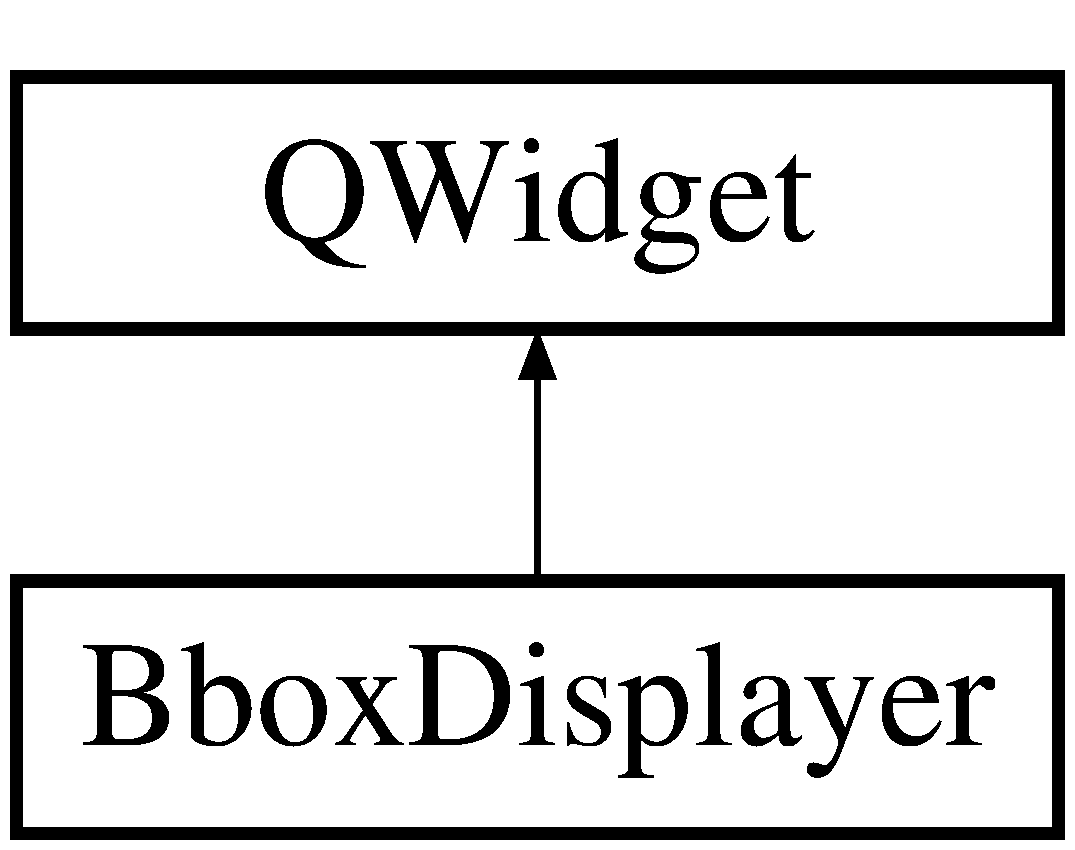
\includegraphics[height=2.000000cm]{class_bbox_displayer}
\end{center}
\end{figure}
\subsection*{Public Slots}
\begin{DoxyCompactItemize}
\item 
void \hyperlink{class_bbox_displayer_a7673afcbb9b907974a1e9880e996fd98}{draw\+Bboxes} ()\hypertarget{class_bbox_displayer_a7673afcbb9b907974a1e9880e996fd98}{}\label{class_bbox_displayer_a7673afcbb9b907974a1e9880e996fd98}

\begin{DoxyCompactList}\small\item\em draws the bboxes in the picture \end{DoxyCompactList}\end{DoxyCompactItemize}
\subsection*{Public Member Functions}
\begin{DoxyCompactItemize}
\item 
{\bfseries Bbox\+Displayer} (Q\+Widget $\ast$parent=0, \hyperlink{class_image_widget}{Image\+Widget} $\ast$image\+Widget=0)\hypertarget{class_bbox_displayer_a90791291ba03e5dbe1ea1e2579f448dc}{}\label{class_bbox_displayer_a90791291ba03e5dbe1ea1e2579f448dc}

\item 
void \hyperlink{class_bbox_displayer_a206b1933a5a48a2798488117dda4a7a1}{add\+Check\+Box} (std\+::string model)
\begin{DoxyCompactList}\small\item\em adds a checkbox to display bbox in the picture \end{DoxyCompactList}\item 
void \hyperlink{class_bbox_displayer_af3c96a831c7585b8ffae51f62f94433a}{clear} ()\hypertarget{class_bbox_displayer_af3c96a831c7585b8ffae51f62f94433a}{}\label{class_bbox_displayer_af3c96a831c7585b8ffae51f62f94433a}

\begin{DoxyCompactList}\small\item\em erases all the checkboxes added \end{DoxyCompactList}\end{DoxyCompactItemize}


\subsection{Detailed Description}
The Widget that displays checkboxes to draw some \hyperlink{class_bbox}{Bbox}. 

\subsection{Member Function Documentation}
\index{Bbox\+Displayer@{Bbox\+Displayer}!add\+Check\+Box@{add\+Check\+Box}}
\index{add\+Check\+Box@{add\+Check\+Box}!Bbox\+Displayer@{Bbox\+Displayer}}
\subsubsection[{\texorpdfstring{add\+Check\+Box(std\+::string model)}{addCheckBox(std::string model)}}]{\setlength{\rightskip}{0pt plus 5cm}void Bbox\+Displayer\+::add\+Check\+Box (
\begin{DoxyParamCaption}
\item[{std\+::string}]{model}
\end{DoxyParamCaption}
)}\hypertarget{class_bbox_displayer_a206b1933a5a48a2798488117dda4a7a1}{}\label{class_bbox_displayer_a206b1933a5a48a2798488117dda4a7a1}


adds a checkbox to display bbox in the picture 


\begin{DoxyParams}{Parameters}
{\em model} & the model name that made the detections \\
\hline
\end{DoxyParams}


The documentation for this class was generated from the following files\+:\begin{DoxyCompactItemize}
\item 
bboxdisplayer.\+h\item 
bboxdisplayer.\+cpp\end{DoxyCompactItemize}

\hypertarget{classtinyxml2_1_1_dyn_array}{}\section{tinyxml2\+:\+:Dyn\+Array$<$ T, I\+N\+I\+T\+I\+A\+L\+\_\+\+S\+I\+ZE $>$ Class Template Reference}
\label{classtinyxml2_1_1_dyn_array}\index{tinyxml2\+::\+Dyn\+Array$<$ T, I\+N\+I\+T\+I\+A\+L\+\_\+\+S\+I\+Z\+E $>$@{tinyxml2\+::\+Dyn\+Array$<$ T, I\+N\+I\+T\+I\+A\+L\+\_\+\+S\+I\+Z\+E $>$}}
\subsection*{Public Member Functions}
\begin{DoxyCompactItemize}
\item 
void {\bfseries Clear} ()\hypertarget{classtinyxml2_1_1_dyn_array_af87a804cd831226d069274b44b74b8bc}{}\label{classtinyxml2_1_1_dyn_array_af87a804cd831226d069274b44b74b8bc}

\item 
void {\bfseries Push} (T t)\hypertarget{classtinyxml2_1_1_dyn_array_aea7ffe983b5d3284bd43171afd7c99d0}{}\label{classtinyxml2_1_1_dyn_array_aea7ffe983b5d3284bd43171afd7c99d0}

\item 
T $\ast$ {\bfseries Push\+Arr} (int count)\hypertarget{classtinyxml2_1_1_dyn_array_ad289abee8cd02b26e215f1b63d2043f1}{}\label{classtinyxml2_1_1_dyn_array_ad289abee8cd02b26e215f1b63d2043f1}

\item 
T {\bfseries Pop} ()\hypertarget{classtinyxml2_1_1_dyn_array_a27a3f2f6f869815b6eabb3ea40cf0712}{}\label{classtinyxml2_1_1_dyn_array_a27a3f2f6f869815b6eabb3ea40cf0712}

\item 
void {\bfseries Pop\+Arr} (int count)\hypertarget{classtinyxml2_1_1_dyn_array_ab8b8c94a2312ab27e2846f0d61ef677a}{}\label{classtinyxml2_1_1_dyn_array_ab8b8c94a2312ab27e2846f0d61ef677a}

\item 
bool {\bfseries Empty} () const \hypertarget{classtinyxml2_1_1_dyn_array_a1c6766bdf61c2d3c2b95dab146ab48b9}{}\label{classtinyxml2_1_1_dyn_array_a1c6766bdf61c2d3c2b95dab146ab48b9}

\item 
T \& {\bfseries operator\mbox{[}$\,$\mbox{]}} (int i)\hypertarget{classtinyxml2_1_1_dyn_array_a756cf4e7464c711aa720e2b17a251daa}{}\label{classtinyxml2_1_1_dyn_array_a756cf4e7464c711aa720e2b17a251daa}

\item 
const T \& {\bfseries operator\mbox{[}$\,$\mbox{]}} (int i) const \hypertarget{classtinyxml2_1_1_dyn_array_ac97d6ddabbcdb098f155e7fc11ea5d91}{}\label{classtinyxml2_1_1_dyn_array_ac97d6ddabbcdb098f155e7fc11ea5d91}

\item 
const T \& {\bfseries Peek\+Top} () const \hypertarget{classtinyxml2_1_1_dyn_array_a5658d49c056707f14b089b53c358eb11}{}\label{classtinyxml2_1_1_dyn_array_a5658d49c056707f14b089b53c358eb11}

\item 
int {\bfseries Size} () const \hypertarget{classtinyxml2_1_1_dyn_array_a5c3874dd4d5d0bf32919161b19ac7287}{}\label{classtinyxml2_1_1_dyn_array_a5c3874dd4d5d0bf32919161b19ac7287}

\item 
int {\bfseries Capacity} () const \hypertarget{classtinyxml2_1_1_dyn_array_a5ab6ef31e984e5cf78d0eb70ad3aec6d}{}\label{classtinyxml2_1_1_dyn_array_a5ab6ef31e984e5cf78d0eb70ad3aec6d}

\item 
const T $\ast$ {\bfseries Mem} () const \hypertarget{classtinyxml2_1_1_dyn_array_aef95a07fb624948d8ce3e638ab2e1f8b}{}\label{classtinyxml2_1_1_dyn_array_aef95a07fb624948d8ce3e638ab2e1f8b}

\item 
T $\ast$ {\bfseries Mem} ()\hypertarget{classtinyxml2_1_1_dyn_array_a2f0842cd666e2ad951f1a8bd6561fa40}{}\label{classtinyxml2_1_1_dyn_array_a2f0842cd666e2ad951f1a8bd6561fa40}

\end{DoxyCompactItemize}


The documentation for this class was generated from the following file\+:\begin{DoxyCompactItemize}
\item 
tinyxml2.\+h\end{DoxyCompactItemize}

\hypertarget{structtinyxml2_1_1_entity}{}\section{tinyxml2\+:\+:Entity Struct Reference}
\label{structtinyxml2_1_1_entity}\index{tinyxml2\+::\+Entity@{tinyxml2\+::\+Entity}}
\subsection*{Public Attributes}
\begin{DoxyCompactItemize}
\item 
const char $\ast$ {\bfseries pattern}\hypertarget{structtinyxml2_1_1_entity_ab330f5d665d29bfc811ecfa76315894b}{}\label{structtinyxml2_1_1_entity_ab330f5d665d29bfc811ecfa76315894b}

\item 
int {\bfseries length}\hypertarget{structtinyxml2_1_1_entity_a25e2b57cb59cb4fa68f283d7cb570f21}{}\label{structtinyxml2_1_1_entity_a25e2b57cb59cb4fa68f283d7cb570f21}

\item 
char {\bfseries value}\hypertarget{structtinyxml2_1_1_entity_a7334e81e33b4615655a403711b24f3ed}{}\label{structtinyxml2_1_1_entity_a7334e81e33b4615655a403711b24f3ed}

\end{DoxyCompactItemize}


The documentation for this struct was generated from the following file\+:\begin{DoxyCompactItemize}
\item 
src/tinyxml2.\+cpp\end{DoxyCompactItemize}

\hypertarget{class_image}{}\section{Image Class Reference}
\label{class_image}\index{Image@{Image}}


The \hyperlink{class_image}{Image} class contains all the information about the objects in it etc.  




{\ttfamily \#include $<$image.\+h$>$}

\subsection*{Public Member Functions}
\begin{DoxyCompactItemize}
\item 
\hyperlink{class_image_a02455aeac6921a752aee20d1697ca162}{Image} (std\+::string file\+Name)
\begin{DoxyCompactList}\small\item\em Builds an \hyperlink{class_image}{Image} given a line divided into substrings. \end{DoxyCompactList}\item 
void \hyperlink{class_image_a6f2d732f8c5c253a511d6bbbdaf6d64a}{add\+Object} (\hyperlink{class_object}{Object} object)
\begin{DoxyCompactList}\small\item\em adds an object detected to this image \end{DoxyCompactList}\item 
std\+::string \hyperlink{class_image_a6546fe9d1f1b8bd456370a64816d1e5f}{get\+File\+Name} ()
\begin{DoxyCompactList}\small\item\em Accessor to the file name of the picture. \end{DoxyCompactList}\item 
std\+::vector$<$ \hyperlink{class_object}{Object} $>$ \hyperlink{class_image_a4a981047292f47239383d6bbcd946b4d}{get\+Objects} ()\hypertarget{class_image_a4a981047292f47239383d6bbcd946b4d}{}\label{class_image_a4a981047292f47239383d6bbcd946b4d}

\begin{DoxyCompactList}\small\item\em gets the objects detected in the picture \end{DoxyCompactList}\end{DoxyCompactItemize}


\subsection{Detailed Description}
The \hyperlink{class_image}{Image} class contains all the information about the objects in it etc. 

\subsection{Constructor \& Destructor Documentation}
\index{Image@{Image}!Image@{Image}}
\index{Image@{Image}!Image@{Image}}
\subsubsection[{\texorpdfstring{Image(std\+::string file\+Name)}{Image(std::string fileName)}}]{\setlength{\rightskip}{0pt plus 5cm}Image\+::\+Image (
\begin{DoxyParamCaption}
\item[{std\+::string}]{file\+Name}
\end{DoxyParamCaption}
)}\hypertarget{class_image_a02455aeac6921a752aee20d1697ca162}{}\label{class_image_a02455aeac6921a752aee20d1697ca162}


Builds an \hyperlink{class_image}{Image} given a line divided into substrings. 


\begin{DoxyParams}{Parameters}
{\em file\+Name} & the name of the file that is the picture \\
\hline
\end{DoxyParams}


\subsection{Member Function Documentation}
\index{Image@{Image}!add\+Object@{add\+Object}}
\index{add\+Object@{add\+Object}!Image@{Image}}
\subsubsection[{\texorpdfstring{add\+Object(\+Object object)}{addObject(Object object)}}]{\setlength{\rightskip}{0pt plus 5cm}void Image\+::add\+Object (
\begin{DoxyParamCaption}
\item[{{\bf Object}}]{object}
\end{DoxyParamCaption}
)}\hypertarget{class_image_a6f2d732f8c5c253a511d6bbbdaf6d64a}{}\label{class_image_a6f2d732f8c5c253a511d6bbbdaf6d64a}


adds an object detected to this image 


\begin{DoxyParams}{Parameters}
{\em object} & th eobject added \\
\hline
\end{DoxyParams}
\index{Image@{Image}!get\+File\+Name@{get\+File\+Name}}
\index{get\+File\+Name@{get\+File\+Name}!Image@{Image}}
\subsubsection[{\texorpdfstring{get\+File\+Name()}{getFileName()}}]{\setlength{\rightskip}{0pt plus 5cm}string Image\+::get\+File\+Name (
\begin{DoxyParamCaption}
{}
\end{DoxyParamCaption}
)}\hypertarget{class_image_a6546fe9d1f1b8bd456370a64816d1e5f}{}\label{class_image_a6546fe9d1f1b8bd456370a64816d1e5f}


Accessor to the file name of the picture. 

\begin{DoxyReturn}{Returns}
a string giving the file name 
\end{DoxyReturn}


The documentation for this class was generated from the following files\+:\begin{DoxyCompactItemize}
\item 
src/image.\+h\item 
src/image.\+cpp\end{DoxyCompactItemize}

\hypertarget{class_image_displayer}{}\section{Image\+Displayer Class Reference}
\label{class_image_displayer}\index{Image\+Displayer@{Image\+Displayer}}


Containing widget to display the image, and the options to see the results od detection in it.  




{\ttfamily \#include $<$imagedisplayer.\+h$>$}

Inheritance diagram for Image\+Displayer\+:\begin{figure}[H]
\begin{center}
\leavevmode
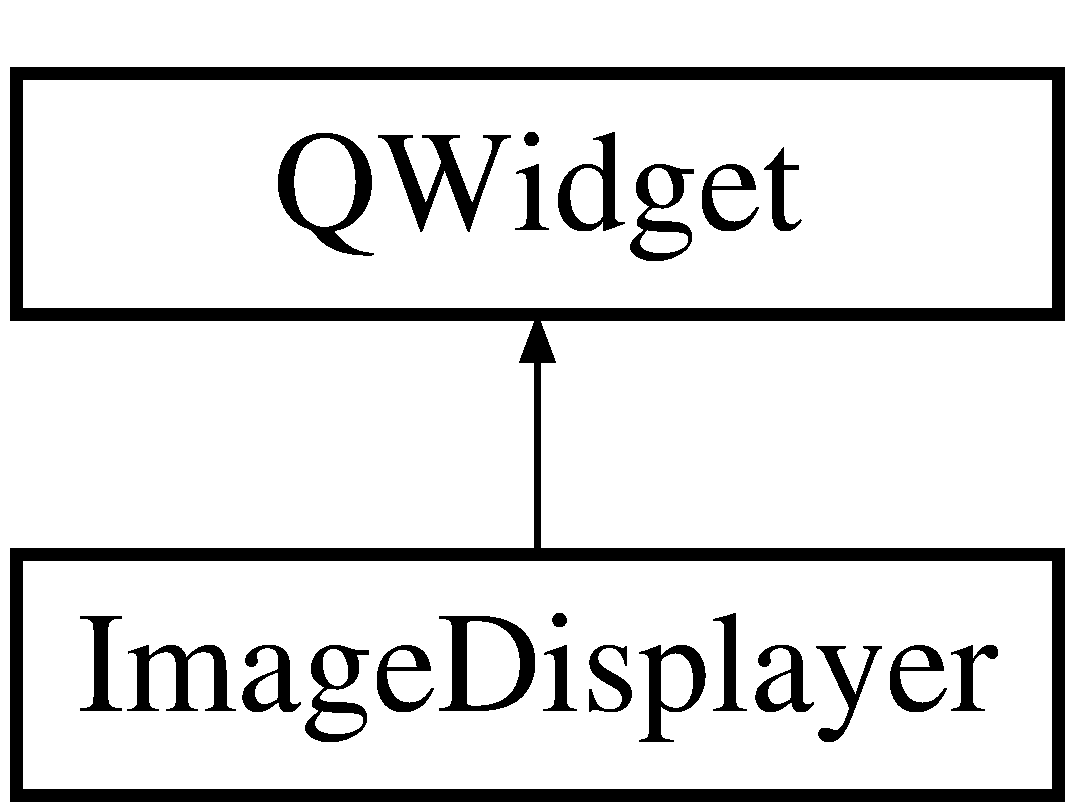
\includegraphics[height=2.000000cm]{class_image_displayer}
\end{center}
\end{figure}
\subsection*{Public Slots}
\begin{DoxyCompactItemize}
\item 
void \hyperlink{class_image_displayer_a9a57980fbe20b55a59f3c189275c3f47}{next\+Image} ()\hypertarget{class_image_displayer_a9a57980fbe20b55a59f3c189275c3f47}{}\label{class_image_displayer_a9a57980fbe20b55a59f3c189275c3f47}

\begin{DoxyCompactList}\small\item\em Goes to the next image and loop back to 1st when at the end. \end{DoxyCompactList}\item 
void \hyperlink{class_image_displayer_a32b7d20ab0b8959fd08580a2855ff74f}{prev\+Image} ()\hypertarget{class_image_displayer_a32b7d20ab0b8959fd08580a2855ff74f}{}\label{class_image_displayer_a32b7d20ab0b8959fd08580a2855ff74f}

\begin{DoxyCompactList}\small\item\em prev\+Image Goes to previous image and loop to the end when 1st reached \end{DoxyCompactList}\item 
void \hyperlink{class_image_displayer_a34877e02ed6399153428be9ba4c9474a}{update\+Slider\+Value} (int int\+Value)
\begin{DoxyCompactList}\small\item\em updates the slider\textquotesingle{}s value \end{DoxyCompactList}\item 
void \hyperlink{class_image_displayer_acb3df03f56e022a8814484923594a916}{go\+To\+File} ()\hypertarget{class_image_displayer_acb3df03f56e022a8814484923594a916}{}\label{class_image_displayer_acb3df03f56e022a8814484923594a916}

\begin{DoxyCompactList}\small\item\em goes to a file chosen by the user \end{DoxyCompactList}\end{DoxyCompactItemize}
\subsection*{Public Member Functions}
\begin{DoxyCompactItemize}
\item 
{\bfseries Image\+Displayer} (Q\+Widget $\ast$parent=0)\hypertarget{class_image_displayer_ab368441dea5815d4c623744599d9761f}{}\label{class_image_displayer_ab368441dea5815d4c623744599d9761f}

\item 
void \hyperlink{class_image_displayer_a57a0e59aec7694beac57bbf667fe46a3}{set\+Results} (\hyperlink{class_results}{Results} $\ast$results)
\begin{DoxyCompactList}\small\item\em sets the results sets of the image displayer \end{DoxyCompactList}\item 
void \hyperlink{class_image_displayer_a3b9b38db521f0355d54f7bb90c1b4006}{fetch\+Images} ()\hypertarget{class_image_displayer_a3b9b38db521f0355d54f7bb90c1b4006}{}\label{class_image_displayer_a3b9b38db521f0355d54f7bb90c1b4006}

\begin{DoxyCompactList}\small\item\em The displayer fetches his results to update the images displayed. \end{DoxyCompactList}\end{DoxyCompactItemize}


\subsection{Detailed Description}
Containing widget to display the image, and the options to see the results od detection in it. 

\subsection{Member Function Documentation}
\index{Image\+Displayer@{Image\+Displayer}!set\+Results@{set\+Results}}
\index{set\+Results@{set\+Results}!Image\+Displayer@{Image\+Displayer}}
\subsubsection[{\texorpdfstring{set\+Results(\+Results $\ast$results)}{setResults(Results *results)}}]{\setlength{\rightskip}{0pt plus 5cm}void Image\+Displayer\+::set\+Results (
\begin{DoxyParamCaption}
\item[{{\bf Results} $\ast$}]{results}
\end{DoxyParamCaption}
)}\hypertarget{class_image_displayer_a57a0e59aec7694beac57bbf667fe46a3}{}\label{class_image_displayer_a57a0e59aec7694beac57bbf667fe46a3}


sets the results sets of the image displayer 


\begin{DoxyParams}{Parameters}
{\em results} & the results to be set \\
\hline
\end{DoxyParams}
\index{Image\+Displayer@{Image\+Displayer}!update\+Slider\+Value@{update\+Slider\+Value}}
\index{update\+Slider\+Value@{update\+Slider\+Value}!Image\+Displayer@{Image\+Displayer}}
\subsubsection[{\texorpdfstring{update\+Slider\+Value}{updateSliderValue}}]{\setlength{\rightskip}{0pt plus 5cm}void Image\+Displayer\+::update\+Slider\+Value (
\begin{DoxyParamCaption}
\item[{int}]{int\+Value}
\end{DoxyParamCaption}
)\hspace{0.3cm}{\ttfamily [slot]}}\hypertarget{class_image_displayer_a34877e02ed6399153428be9ba4c9474a}{}\label{class_image_displayer_a34877e02ed6399153428be9ba4c9474a}


updates the slider\textquotesingle{}s value 


\begin{DoxyParams}{Parameters}
{\em int\+Value} & the value from 0 to 100 to be converted to float \\
\hline
\end{DoxyParams}


The documentation for this class was generated from the following files\+:\begin{DoxyCompactItemize}
\item 
imagedisplayer.\+h\item 
imagedisplayer.\+cpp\end{DoxyCompactItemize}

\hypertarget{class_image_loader}{}\section{Image\+Loader Class Reference}
\label{class_image_loader}\index{Image\+Loader@{Image\+Loader}}


The \hyperlink{class_image_loader}{Image\+Loader} loads images from an X\+ML file using Tiny\+X\+ML.  




{\ttfamily \#include $<$imageloader.\+h$>$}

\subsection*{Public Member Functions}
\begin{DoxyCompactItemize}
\item 
\hyperlink{class_image_loader_af0e70316989d3992c23ea52cd337c9ad}{Image\+Loader} ()\hypertarget{class_image_loader_af0e70316989d3992c23ea52cd337c9ad}{}\label{class_image_loader_af0e70316989d3992c23ea52cd337c9ad}

\begin{DoxyCompactList}\small\item\em Builds the \hyperlink{class_image}{Image} Loader. \end{DoxyCompactList}\item 
std\+::vector$<$ \hyperlink{class_image}{Image} $>$ \hyperlink{class_image_loader_ae81f649971d3638f12be412dce0fd11f}{load\+Images} (std\+::string file\+Name)
\begin{DoxyCompactList}\small\item\em loads images from a given X\+ML file \end{DoxyCompactList}\end{DoxyCompactItemize}


\subsection{Detailed Description}
The \hyperlink{class_image_loader}{Image\+Loader} loads images from an X\+ML file using Tiny\+X\+ML. 

\subsection{Member Function Documentation}
\index{Image\+Loader@{Image\+Loader}!load\+Images@{load\+Images}}
\index{load\+Images@{load\+Images}!Image\+Loader@{Image\+Loader}}
\subsubsection[{\texorpdfstring{load\+Images(std\+::string file\+Name)}{loadImages(std::string fileName)}}]{\setlength{\rightskip}{0pt plus 5cm}vector$<$ {\bf Image} $>$ Image\+Loader\+::load\+Images (
\begin{DoxyParamCaption}
\item[{std\+::string}]{file\+Name}
\end{DoxyParamCaption}
)}\hypertarget{class_image_loader_ae81f649971d3638f12be412dce0fd11f}{}\label{class_image_loader_ae81f649971d3638f12be412dce0fd11f}


loads images from a given X\+ML file 


\begin{DoxyParams}{Parameters}
{\em file\+Name} & the name of the X\+ML file given \\
\hline
\end{DoxyParams}
\begin{DoxyReturn}{Returns}
a vector of all the images 
\end{DoxyReturn}


The documentation for this class was generated from the following files\+:\begin{DoxyCompactItemize}
\item 
imageloader.\+h\item 
imageloader.\+cpp\end{DoxyCompactItemize}

\hypertarget{class_image_widget}{}\section{Image\+Widget Class Reference}
\label{class_image_widget}\index{Image\+Widget@{Image\+Widget}}


The widget that draws the \hyperlink{class_image}{Image}.  




{\ttfamily \#include $<$imagewidget.\+h$>$}

Inheritance diagram for Image\+Widget\+:\begin{figure}[H]
\begin{center}
\leavevmode
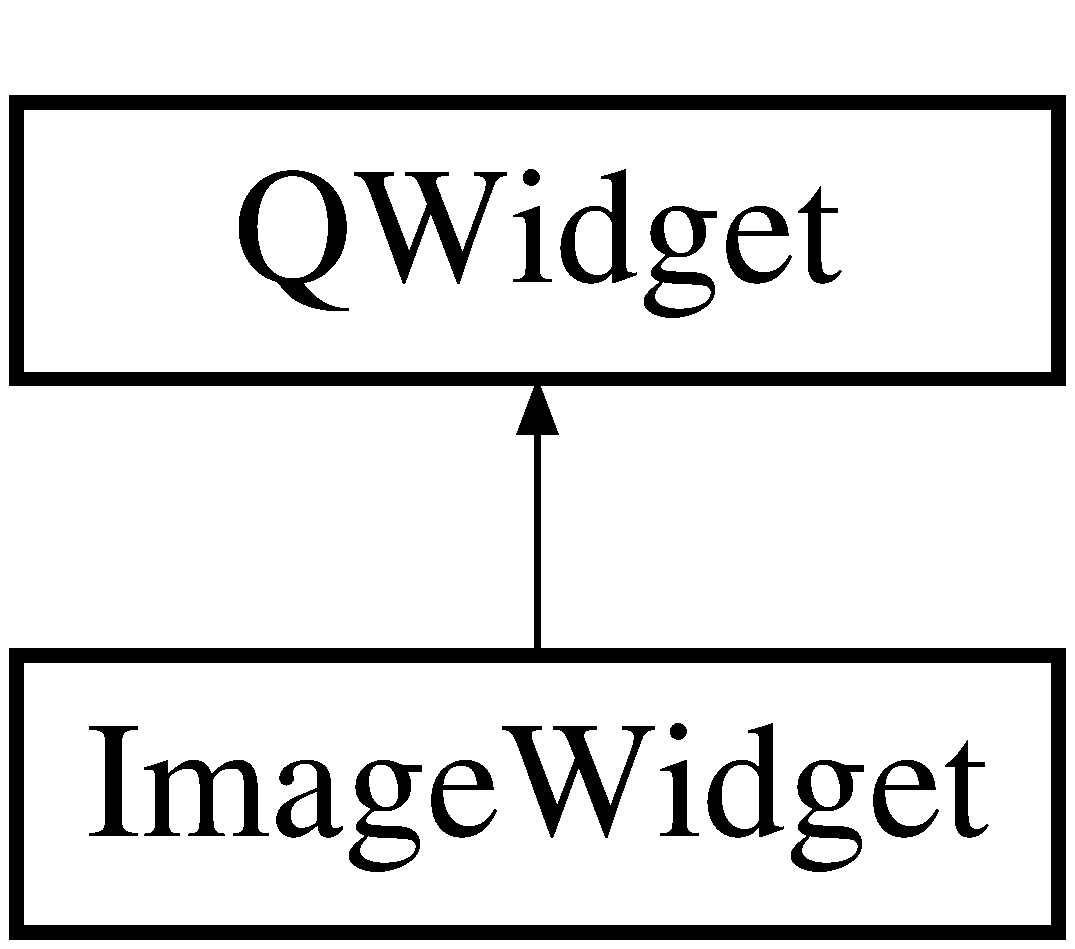
\includegraphics[height=2.000000cm]{class_image_widget}
\end{center}
\end{figure}
\subsection*{Public Member Functions}
\begin{DoxyCompactItemize}
\item 
{\bfseries Image\+Widget} (Q\+Widget $\ast$parent=0)\hypertarget{class_image_widget_a29f5483569b0ac4abd6b25bb640f9250}{}\label{class_image_widget_a29f5483569b0ac4abd6b25bb640f9250}

\item 
void \hyperlink{class_image_widget_a0e3dfd9d7747707f659310b175629e5e}{set\+Results} (\hyperlink{class_results}{Results} $\ast$results)
\begin{DoxyCompactList}\small\item\em sets the results once initiated \end{DoxyCompactList}\item 
void \hyperlink{class_image_widget_ac41822f2c322b22eb62ac553011b0423}{load\+Image} (unsigned int i)
\begin{DoxyCompactList}\small\item\em loads the image n°i in the results sets \end{DoxyCompactList}\item 
void \hyperlink{class_image_widget_a10cd7197e52740e168ef5261aa16ca7a}{paint\+Bbox} ()\hypertarget{class_image_widget_a10cd7197e52740e168ef5261aa16ca7a}{}\label{class_image_widget_a10cd7197e52740e168ef5261aa16ca7a}

\begin{DoxyCompactList}\small\item\em paints the \hyperlink{class_bbox}{Bbox} if some model names have been checked \end{DoxyCompactList}\item 
void \hyperlink{class_image_widget_a774f0d94f4cd8a0ed0d7c8a30b20da56}{set\+Model\+Names} (std\+::map$<$ std\+::string, Q\+Color $>$ model\+Names)
\begin{DoxyCompactList}\small\item\em sets the model names checked with their drawing color \end{DoxyCompactList}\item 
void \hyperlink{class_image_widget_ae572ff8733d9ece83441a37e1b7a91ae}{erase\+Bbox} ()\hypertarget{class_image_widget_ae572ff8733d9ece83441a37e1b7a91ae}{}\label{class_image_widget_ae572ff8733d9ece83441a37e1b7a91ae}

\begin{DoxyCompactList}\small\item\em erases everything that has been drawn \end{DoxyCompactList}\item 
void \hyperlink{class_image_widget_a6180527a08974bc832d10deccc9e3737}{set\+Threshold} (double threshold)
\begin{DoxyCompactList}\small\item\em the new threshold value \end{DoxyCompactList}\end{DoxyCompactItemize}


\subsection{Detailed Description}
The widget that draws the \hyperlink{class_image}{Image}. 

\subsection{Member Function Documentation}
\index{Image\+Widget@{Image\+Widget}!load\+Image@{load\+Image}}
\index{load\+Image@{load\+Image}!Image\+Widget@{Image\+Widget}}
\subsubsection[{\texorpdfstring{load\+Image(unsigned int i)}{loadImage(unsigned int i)}}]{\setlength{\rightskip}{0pt plus 5cm}void Image\+Widget\+::load\+Image (
\begin{DoxyParamCaption}
\item[{unsigned int}]{i}
\end{DoxyParamCaption}
)}\hypertarget{class_image_widget_ac41822f2c322b22eb62ac553011b0423}{}\label{class_image_widget_ac41822f2c322b22eb62ac553011b0423}


loads the image n°i in the results sets 


\begin{DoxyParams}{Parameters}
{\em i} & the index \\
\hline
\end{DoxyParams}
\index{Image\+Widget@{Image\+Widget}!set\+Model\+Names@{set\+Model\+Names}}
\index{set\+Model\+Names@{set\+Model\+Names}!Image\+Widget@{Image\+Widget}}
\subsubsection[{\texorpdfstring{set\+Model\+Names(std\+::map$<$ std\+::string, Q\+Color $>$ model\+Names)}{setModelNames(std::map< std::string, QColor > modelNames)}}]{\setlength{\rightskip}{0pt plus 5cm}void Image\+Widget\+::set\+Model\+Names (
\begin{DoxyParamCaption}
\item[{std\+::map$<$ std\+::string, Q\+Color $>$}]{model\+Names}
\end{DoxyParamCaption}
)}\hypertarget{class_image_widget_a774f0d94f4cd8a0ed0d7c8a30b20da56}{}\label{class_image_widget_a774f0d94f4cd8a0ed0d7c8a30b20da56}


sets the model names checked with their drawing color 


\begin{DoxyParams}{Parameters}
{\em model\+Names} & the model names + color \\
\hline
\end{DoxyParams}
\index{Image\+Widget@{Image\+Widget}!set\+Results@{set\+Results}}
\index{set\+Results@{set\+Results}!Image\+Widget@{Image\+Widget}}
\subsubsection[{\texorpdfstring{set\+Results(\+Results $\ast$results)}{setResults(Results *results)}}]{\setlength{\rightskip}{0pt plus 5cm}void Image\+Widget\+::set\+Results (
\begin{DoxyParamCaption}
\item[{{\bf Results} $\ast$}]{results}
\end{DoxyParamCaption}
)}\hypertarget{class_image_widget_a0e3dfd9d7747707f659310b175629e5e}{}\label{class_image_widget_a0e3dfd9d7747707f659310b175629e5e}


sets the results once initiated 


\begin{DoxyParams}{Parameters}
{\em results} & the results to be linked \\
\hline
\end{DoxyParams}
\index{Image\+Widget@{Image\+Widget}!set\+Threshold@{set\+Threshold}}
\index{set\+Threshold@{set\+Threshold}!Image\+Widget@{Image\+Widget}}
\subsubsection[{\texorpdfstring{set\+Threshold(double threshold)}{setThreshold(double threshold)}}]{\setlength{\rightskip}{0pt plus 5cm}void Image\+Widget\+::set\+Threshold (
\begin{DoxyParamCaption}
\item[{double}]{threshold}
\end{DoxyParamCaption}
)}\hypertarget{class_image_widget_a6180527a08974bc832d10deccc9e3737}{}\label{class_image_widget_a6180527a08974bc832d10deccc9e3737}


the new threshold value 


\begin{DoxyParams}{Parameters}
{\em threshold} & the threshold value \\
\hline
\end{DoxyParams}


The documentation for this class was generated from the following files\+:\begin{DoxyCompactItemize}
\item 
imagewidget.\+h\item 
imagewidget.\+cpp\end{DoxyCompactItemize}

\hypertarget{structtinyxml2_1_1_long_fits_into_size_t_minus_one}{}\section{tinyxml2\+:\+:Long\+Fits\+Into\+Size\+T\+Minus\+One$<$ bool $>$ Struct Template Reference}
\label{structtinyxml2_1_1_long_fits_into_size_t_minus_one}\index{tinyxml2\+::\+Long\+Fits\+Into\+Size\+T\+Minus\+One$<$ bool $>$@{tinyxml2\+::\+Long\+Fits\+Into\+Size\+T\+Minus\+One$<$ bool $>$}}
\subsection*{Public Member Functions}
\begin{DoxyCompactItemize}
\item 
{\footnotesize template$<$$>$ }\\bool {\bfseries Fits} (unsigned long)\hypertarget{structtinyxml2_1_1_long_fits_into_size_t_minus_one_a85fb9734fefa25d130ea831f683fc444}{}\label{structtinyxml2_1_1_long_fits_into_size_t_minus_one_a85fb9734fefa25d130ea831f683fc444}

\end{DoxyCompactItemize}
\subsection*{Static Public Member Functions}
\begin{DoxyCompactItemize}
\item 
static bool {\bfseries Fits} (unsigned long value)\hypertarget{structtinyxml2_1_1_long_fits_into_size_t_minus_one_a3057710104ab733963eb32fda0bc374c}{}\label{structtinyxml2_1_1_long_fits_into_size_t_minus_one_a3057710104ab733963eb32fda0bc374c}

\end{DoxyCompactItemize}


The documentation for this struct was generated from the following file\+:\begin{DoxyCompactItemize}
\item 
src/tinyxml2.\+cpp\end{DoxyCompactItemize}

\hypertarget{class_main_window}{}\section{Main\+Window Class Reference}
\label{class_main_window}\index{Main\+Window@{Main\+Window}}
Inheritance diagram for Main\+Window\+:\begin{figure}[H]
\begin{center}
\leavevmode
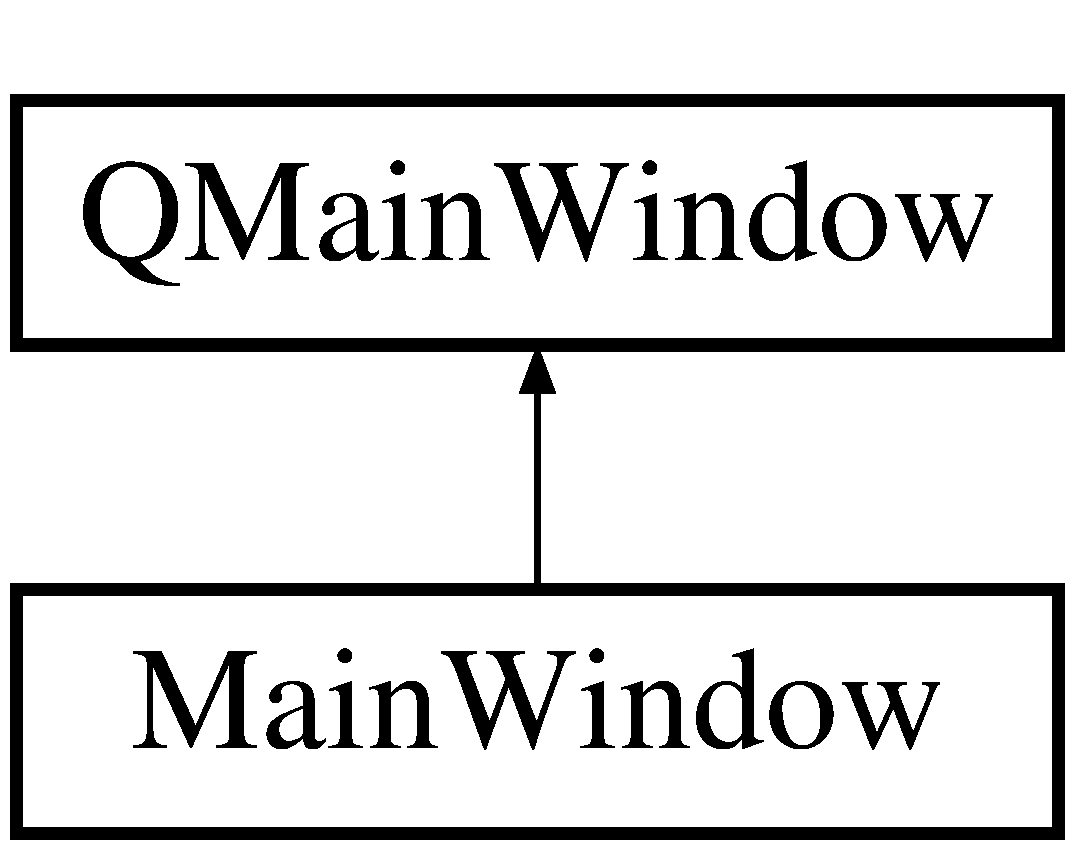
\includegraphics[height=2.000000cm]{class_main_window}
\end{center}
\end{figure}
\subsection*{Public Slots}
\begin{DoxyCompactItemize}
\item 
void \hyperlink{class_main_window_ab231326d40a58616a2a6c194a95f40af}{validate\+Enabler} (Q\+String data)
\begin{DoxyCompactList}\small\item\em enables the validation button when the text is filled \end{DoxyCompactList}\item 
void \hyperlink{class_main_window_afc77791f1b130480a0c9364a999283d7}{lock\+Validation} ()\hypertarget{class_main_window_afc77791f1b130480a0c9364a999283d7}{}\label{class_main_window_afc77791f1b130480a0c9364a999283d7}

\begin{DoxyCompactList}\small\item\em When the dataset has been named it is locked. \end{DoxyCompactList}\item 
void \hyperlink{class_main_window_aa2762bc39780ff9bc5c533ef4581d07d}{search\+Folder} ()\hypertarget{class_main_window_aa2762bc39780ff9bc5c533ef4581d07d}{}\label{class_main_window_aa2762bc39780ff9bc5c533ef4581d07d}

\begin{DoxyCompactList}\small\item\em searches the folder of the dataset using a Q\+File\+Dialog \end{DoxyCompactList}\end{DoxyCompactItemize}
\subsection*{Public Member Functions}
\begin{DoxyCompactItemize}
\item 
{\bfseries Main\+Window} (Q\+Widget $\ast$parent=0)\hypertarget{class_main_window_a8b244be8b7b7db1b08de2a2acb9409db}{}\label{class_main_window_a8b244be8b7b7db1b08de2a2acb9409db}

\end{DoxyCompactItemize}


\subsection{Member Function Documentation}
\index{Main\+Window@{Main\+Window}!validate\+Enabler@{validate\+Enabler}}
\index{validate\+Enabler@{validate\+Enabler}!Main\+Window@{Main\+Window}}
\subsubsection[{\texorpdfstring{validate\+Enabler}{validateEnabler}}]{\setlength{\rightskip}{0pt plus 5cm}void Main\+Window\+::validate\+Enabler (
\begin{DoxyParamCaption}
\item[{Q\+String}]{data}
\end{DoxyParamCaption}
)\hspace{0.3cm}{\ttfamily [slot]}}\hypertarget{class_main_window_ab231326d40a58616a2a6c194a95f40af}{}\label{class_main_window_ab231326d40a58616a2a6c194a95f40af}


enables the validation button when the text is filled 


\begin{DoxyParams}{Parameters}
{\em data} & the string of the text field \\
\hline
\end{DoxyParams}


The documentation for this class was generated from the following files\+:\begin{DoxyCompactItemize}
\item 
mainwindow.\+h\item 
mainwindow.\+cpp\end{DoxyCompactItemize}

\hypertarget{classtinyxml2_1_1_mem_pool}{}\section{tinyxml2\+:\+:Mem\+Pool Class Reference}
\label{classtinyxml2_1_1_mem_pool}\index{tinyxml2\+::\+Mem\+Pool@{tinyxml2\+::\+Mem\+Pool}}
Inheritance diagram for tinyxml2\+:\+:Mem\+Pool\+:\begin{figure}[H]
\begin{center}
\leavevmode
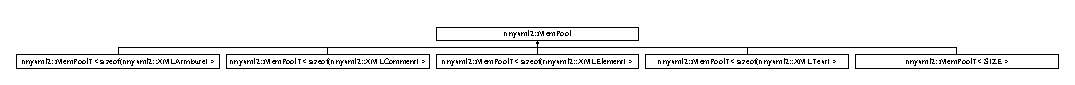
\includegraphics[height=0.691358cm]{classtinyxml2_1_1_mem_pool}
\end{center}
\end{figure}
\subsection*{Public Member Functions}
\begin{DoxyCompactItemize}
\item 
virtual int {\bfseries Item\+Size} () const  =0\hypertarget{classtinyxml2_1_1_mem_pool_afb3d8c6cbe91b44f90043d0d94dc7306}{}\label{classtinyxml2_1_1_mem_pool_afb3d8c6cbe91b44f90043d0d94dc7306}

\item 
virtual void $\ast$ {\bfseries Alloc} ()=0\hypertarget{classtinyxml2_1_1_mem_pool_a4f977b5fed752c0bbfe5295f469d6449}{}\label{classtinyxml2_1_1_mem_pool_a4f977b5fed752c0bbfe5295f469d6449}

\item 
virtual void {\bfseries Free} (void $\ast$)=0\hypertarget{classtinyxml2_1_1_mem_pool_a49e3bfac2cba2ebd6776b31e571f64f7}{}\label{classtinyxml2_1_1_mem_pool_a49e3bfac2cba2ebd6776b31e571f64f7}

\item 
virtual void {\bfseries Set\+Tracked} ()=0\hypertarget{classtinyxml2_1_1_mem_pool_ac5804dd1387b2e4de5eef710076a0db1}{}\label{classtinyxml2_1_1_mem_pool_ac5804dd1387b2e4de5eef710076a0db1}

\item 
virtual void {\bfseries Clear} ()=0\hypertarget{classtinyxml2_1_1_mem_pool_a74fcdef9756917c8ae19fbbb4d658ed7}{}\label{classtinyxml2_1_1_mem_pool_a74fcdef9756917c8ae19fbbb4d658ed7}

\end{DoxyCompactItemize}


The documentation for this class was generated from the following file\+:\begin{DoxyCompactItemize}
\item 
tinyxml2.\+h\end{DoxyCompactItemize}

\hypertarget{classtinyxml2_1_1_mem_pool_t}{}\section{tinyxml2\+:\+:Mem\+PoolT$<$ S\+I\+ZE $>$ Class Template Reference}
\label{classtinyxml2_1_1_mem_pool_t}\index{tinyxml2\+::\+Mem\+Pool\+T$<$ S\+I\+Z\+E $>$@{tinyxml2\+::\+Mem\+Pool\+T$<$ S\+I\+Z\+E $>$}}
Inheritance diagram for tinyxml2\+:\+:Mem\+PoolT$<$ S\+I\+ZE $>$\+:\begin{figure}[H]
\begin{center}
\leavevmode
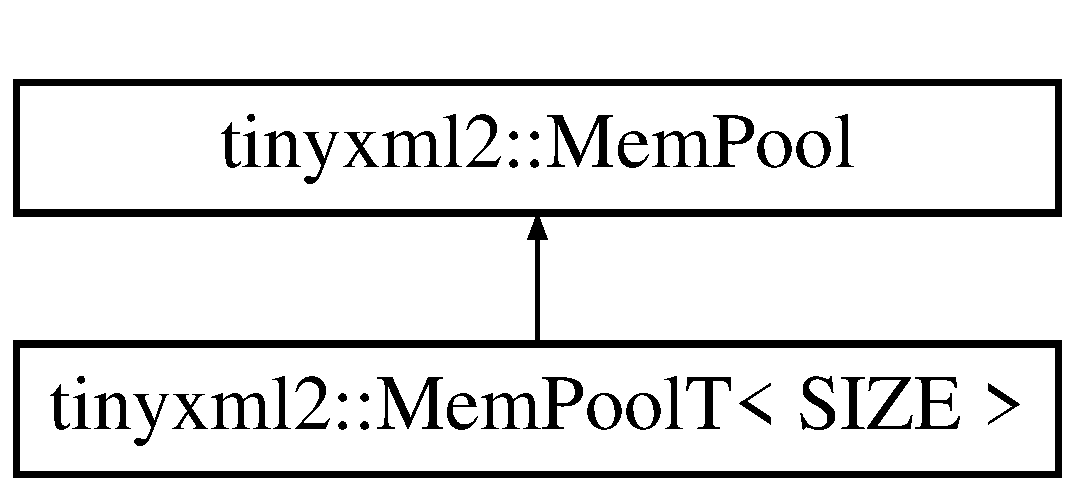
\includegraphics[height=2.000000cm]{classtinyxml2_1_1_mem_pool_t}
\end{center}
\end{figure}
\subsection*{Public Types}
\begin{DoxyCompactItemize}
\item 
enum \{ {\bfseries C\+O\+U\+NT} = (4$\ast$1024)/\+S\+I\+ZE
 \}\hypertarget{classtinyxml2_1_1_mem_pool_t_a04cf45156e6f913f93972869ff8a1d94}{}\label{classtinyxml2_1_1_mem_pool_t_a04cf45156e6f913f93972869ff8a1d94}

\end{DoxyCompactItemize}
\subsection*{Public Member Functions}
\begin{DoxyCompactItemize}
\item 
void {\bfseries Clear} ()\hypertarget{classtinyxml2_1_1_mem_pool_t_a469d55e82be97d5ffeff82dd001a7029}{}\label{classtinyxml2_1_1_mem_pool_t_a469d55e82be97d5ffeff82dd001a7029}

\item 
virtual int {\bfseries Item\+Size} () const \hypertarget{classtinyxml2_1_1_mem_pool_t_a7ec8778fe99f6e332615a703be0b48bc}{}\label{classtinyxml2_1_1_mem_pool_t_a7ec8778fe99f6e332615a703be0b48bc}

\item 
int {\bfseries Current\+Allocs} () const \hypertarget{classtinyxml2_1_1_mem_pool_t_a56be11b7db6a7ef00db17088a7769aab}{}\label{classtinyxml2_1_1_mem_pool_t_a56be11b7db6a7ef00db17088a7769aab}

\item 
virtual void $\ast$ {\bfseries Alloc} ()\hypertarget{classtinyxml2_1_1_mem_pool_t_aa9d785a48ffe6ea1be679bab13464486}{}\label{classtinyxml2_1_1_mem_pool_t_aa9d785a48ffe6ea1be679bab13464486}

\item 
virtual void {\bfseries Free} (void $\ast$mem)\hypertarget{classtinyxml2_1_1_mem_pool_t_a4f1a0c434e9e3d7391e5c16ed4ee8c70}{}\label{classtinyxml2_1_1_mem_pool_t_a4f1a0c434e9e3d7391e5c16ed4ee8c70}

\item 
void {\bfseries Trace} (const char $\ast$name)\hypertarget{classtinyxml2_1_1_mem_pool_t_a0bc596f271e0f139822c534238b3f244}{}\label{classtinyxml2_1_1_mem_pool_t_a0bc596f271e0f139822c534238b3f244}

\item 
void {\bfseries Set\+Tracked} ()\hypertarget{classtinyxml2_1_1_mem_pool_t_a7798932414916199a1bc0f9c3f368521}{}\label{classtinyxml2_1_1_mem_pool_t_a7798932414916199a1bc0f9c3f368521}

\item 
int {\bfseries Untracked} () const \hypertarget{classtinyxml2_1_1_mem_pool_t_a524b90d0edeac41964c06510757dce0f}{}\label{classtinyxml2_1_1_mem_pool_t_a524b90d0edeac41964c06510757dce0f}

\end{DoxyCompactItemize}


The documentation for this class was generated from the following file\+:\begin{DoxyCompactItemize}
\item 
src/tinyxml2.\+h\end{DoxyCompactItemize}

\hypertarget{class_object}{}\section{Object Class Reference}
\label{class_object}\index{Object@{Object}}


An object in a picture.  




{\ttfamily \#include $<$image.\+h$>$}

\subsection*{Public Member Functions}
\begin{DoxyCompactItemize}
\item 
\hyperlink{class_object_ab3e642ef6f10a138adc9d519979d2944}{Object} (std\+::string label, double confidence, \hyperlink{class_bbox}{Bbox} bbox)
\begin{DoxyCompactList}\small\item\em Builds an object with his label and the bounding box around him. \end{DoxyCompactList}\item 
\hyperlink{class_bbox}{Bbox} \hyperlink{class_object_a8fde7ce6bc7c391ff9b87b3557c9bb80}{get\+Bbox} ()
\begin{DoxyCompactList}\small\item\em getter of the \hyperlink{class_bbox}{Bbox} of the object \end{DoxyCompactList}\item 
std\+::string \hyperlink{class_object_a269462ff63fbdb49c1072936b13146a4}{get\+Label} ()
\begin{DoxyCompactList}\small\item\em getter to the label of the object \end{DoxyCompactList}\item 
double \hyperlink{class_object_aa49a09c5b33126340f35eb4ecc0ebf96}{get\+Confidence} ()
\begin{DoxyCompactList}\small\item\em getter to the confidence of this object in the picture \end{DoxyCompactList}\end{DoxyCompactItemize}


\subsection{Detailed Description}
An object in a picture. 

\subsection{Constructor \& Destructor Documentation}
\index{Object@{Object}!Object@{Object}}
\index{Object@{Object}!Object@{Object}}
\subsubsection[{\texorpdfstring{Object(std\+::string label, double confidence, Bbox bbox)}{Object(std::string label, double confidence, Bbox bbox)}}]{\setlength{\rightskip}{0pt plus 5cm}Object\+::\+Object (
\begin{DoxyParamCaption}
\item[{std\+::string}]{label, }
\item[{double}]{confidence, }
\item[{{\bf Bbox}}]{bbox}
\end{DoxyParamCaption}
)}\hypertarget{class_object_ab3e642ef6f10a138adc9d519979d2944}{}\label{class_object_ab3e642ef6f10a138adc9d519979d2944}


Builds an object with his label and the bounding box around him. 


\begin{DoxyParams}{Parameters}
{\em label} & the name of the object \\
\hline
{\em confidence} & the confidence score of detection \\
\hline
{\em bbox} & the bounding box around the object \\
\hline
\end{DoxyParams}


\subsection{Member Function Documentation}
\index{Object@{Object}!get\+Bbox@{get\+Bbox}}
\index{get\+Bbox@{get\+Bbox}!Object@{Object}}
\subsubsection[{\texorpdfstring{get\+Bbox()}{getBbox()}}]{\setlength{\rightskip}{0pt plus 5cm}{\bf Bbox} Object\+::get\+Bbox (
\begin{DoxyParamCaption}
{}
\end{DoxyParamCaption}
)}\hypertarget{class_object_a8fde7ce6bc7c391ff9b87b3557c9bb80}{}\label{class_object_a8fde7ce6bc7c391ff9b87b3557c9bb80}


getter of the \hyperlink{class_bbox}{Bbox} of the object 

\begin{DoxyReturn}{Returns}
the \hyperlink{class_bbox}{Bbox} of the object 
\end{DoxyReturn}
\index{Object@{Object}!get\+Confidence@{get\+Confidence}}
\index{get\+Confidence@{get\+Confidence}!Object@{Object}}
\subsubsection[{\texorpdfstring{get\+Confidence()}{getConfidence()}}]{\setlength{\rightskip}{0pt plus 5cm}double Object\+::get\+Confidence (
\begin{DoxyParamCaption}
{}
\end{DoxyParamCaption}
)}\hypertarget{class_object_aa49a09c5b33126340f35eb4ecc0ebf96}{}\label{class_object_aa49a09c5b33126340f35eb4ecc0ebf96}


getter to the confidence of this object in the picture 

\begin{DoxyReturn}{Returns}
a float value 
\end{DoxyReturn}
\index{Object@{Object}!get\+Label@{get\+Label}}
\index{get\+Label@{get\+Label}!Object@{Object}}
\subsubsection[{\texorpdfstring{get\+Label()}{getLabel()}}]{\setlength{\rightskip}{0pt plus 5cm}string Object\+::get\+Label (
\begin{DoxyParamCaption}
{}
\end{DoxyParamCaption}
)}\hypertarget{class_object_a269462ff63fbdb49c1072936b13146a4}{}\label{class_object_a269462ff63fbdb49c1072936b13146a4}


getter to the label of the object 

\begin{DoxyReturn}{Returns}
a string 
\end{DoxyReturn}


The documentation for this class was generated from the following files\+:\begin{DoxyCompactItemize}
\item 
src/image.\+h\item 
src/image.\+cpp\end{DoxyCompactItemize}

\hypertarget{class_results}{}\section{Results Class Reference}
\label{class_results}\index{Results@{Results}}


The \hyperlink{class_results}{Results} contains all the results sets on an entire dataset.  




{\ttfamily \#include $<$resultset.\+h$>$}

\subsection*{Public Member Functions}
\begin{DoxyCompactItemize}
\item 
\hyperlink{class_results_ac627f746e9b1f266c663e7f0c9ff0e6b}{Results} (std\+::string dataset)
\begin{DoxyCompactList}\small\item\em Builds the results. \end{DoxyCompactList}\item 
int \hyperlink{class_results_a34dbd962a31ef9a2e6fddce10ffc5b0e}{add\+Results} (std\+::string name, std\+::vector$<$ \hyperlink{class_image}{Image} $>$ images)
\begin{DoxyCompactList}\small\item\em add results given by an X\+ML file of detection to this dataset \end{DoxyCompactList}\item 
unsigned int \hyperlink{class_results_a61a442d7f227eec1c3be0f883c414f55}{results\+Size} ()
\begin{DoxyCompactList}\small\item\em returns the amount of pictures in the dataset \end{DoxyCompactList}\item 
const \hyperlink{class_result_set}{Result\+Set} \& \hyperlink{class_results_aa4924bf9220fbe2bc4316a28eff84b46}{result\+Set} (unsigned int i)
\begin{DoxyCompactList}\small\item\em Accessor to view a specific resultset. \end{DoxyCompactList}\item 
void \hyperlink{class_results_ab743b3785706d824fd7fcbfe4bffe7d2}{set\+Location} (std\+::string location)
\begin{DoxyCompactList}\small\item\em sets the location of the dataset \end{DoxyCompactList}\item 
std\+::string \hyperlink{class_results_af7e610ff1860b13d382bef3746aa9603}{dataset\+Location} ()
\begin{DoxyCompactList}\small\item\em get the folder string where the pictures are \end{DoxyCompactList}\end{DoxyCompactItemize}


\subsection{Detailed Description}
The \hyperlink{class_results}{Results} contains all the results sets on an entire dataset. 

\subsection{Constructor \& Destructor Documentation}
\index{Results@{Results}!Results@{Results}}
\index{Results@{Results}!Results@{Results}}
\subsubsection[{\texorpdfstring{Results(std\+::string dataset)}{Results(std::string dataset)}}]{\setlength{\rightskip}{0pt plus 5cm}Results\+::\+Results (
\begin{DoxyParamCaption}
\item[{std\+::string}]{dataset}
\end{DoxyParamCaption}
)}\hypertarget{class_results_ac627f746e9b1f266c663e7f0c9ff0e6b}{}\label{class_results_ac627f746e9b1f266c663e7f0c9ff0e6b}


Builds the results. 


\begin{DoxyParams}{Parameters}
{\em dataset} & the dataset that has been processed \\
\hline
\end{DoxyParams}


\subsection{Member Function Documentation}
\index{Results@{Results}!add\+Results@{add\+Results}}
\index{add\+Results@{add\+Results}!Results@{Results}}
\subsubsection[{\texorpdfstring{add\+Results(std\+::string name, std\+::vector$<$ Image $>$ images)}{addResults(std::string name, std::vector< Image > images)}}]{\setlength{\rightskip}{0pt plus 5cm}int Results\+::add\+Results (
\begin{DoxyParamCaption}
\item[{std\+::string}]{name, }
\item[{std\+::vector$<$ {\bf Image} $>$}]{images}
\end{DoxyParamCaption}
)}\hypertarget{class_results_a34dbd962a31ef9a2e6fddce10ffc5b0e}{}\label{class_results_a34dbd962a31ef9a2e6fddce10ffc5b0e}


add results given by an X\+ML file of detection to this dataset 


\begin{DoxyParams}{Parameters}
{\em name} & the name of the model who produced the results \\
\hline
{\em images} & the results of the detection \\
\hline
\end{DoxyParams}
\begin{DoxyReturn}{Returns}
0 if success else its an error code 
\end{DoxyReturn}
\index{Results@{Results}!dataset\+Location@{dataset\+Location}}
\index{dataset\+Location@{dataset\+Location}!Results@{Results}}
\subsubsection[{\texorpdfstring{dataset\+Location()}{datasetLocation()}}]{\setlength{\rightskip}{0pt plus 5cm}string Results\+::dataset\+Location (
\begin{DoxyParamCaption}
{}
\end{DoxyParamCaption}
)}\hypertarget{class_results_af7e610ff1860b13d382bef3746aa9603}{}\label{class_results_af7e610ff1860b13d382bef3746aa9603}


get the folder string where the pictures are 

\begin{DoxyReturn}{Returns}
a std string 
\end{DoxyReturn}
\index{Results@{Results}!result\+Set@{result\+Set}}
\index{result\+Set@{result\+Set}!Results@{Results}}
\subsubsection[{\texorpdfstring{result\+Set(unsigned int i)}{resultSet(unsigned int i)}}]{\setlength{\rightskip}{0pt plus 5cm}const {\bf Result\+Set} \& Results\+::result\+Set (
\begin{DoxyParamCaption}
\item[{unsigned int}]{i}
\end{DoxyParamCaption}
)}\hypertarget{class_results_aa4924bf9220fbe2bc4316a28eff84b46}{}\label{class_results_aa4924bf9220fbe2bc4316a28eff84b46}


Accessor to view a specific resultset. 


\begin{DoxyParams}{Parameters}
{\em i} & the index of accession \\
\hline
\end{DoxyParams}
\begin{DoxyReturn}{Returns}
a constant reference to a result set (read only) 
\end{DoxyReturn}
\index{Results@{Results}!results\+Size@{results\+Size}}
\index{results\+Size@{results\+Size}!Results@{Results}}
\subsubsection[{\texorpdfstring{results\+Size()}{resultsSize()}}]{\setlength{\rightskip}{0pt plus 5cm}unsigned int Results\+::results\+Size (
\begin{DoxyParamCaption}
{}
\end{DoxyParamCaption}
)}\hypertarget{class_results_a61a442d7f227eec1c3be0f883c414f55}{}\label{class_results_a61a442d7f227eec1c3be0f883c414f55}


returns the amount of pictures in the dataset 

\begin{DoxyReturn}{Returns}
an integer 
\end{DoxyReturn}
\index{Results@{Results}!set\+Location@{set\+Location}}
\index{set\+Location@{set\+Location}!Results@{Results}}
\subsubsection[{\texorpdfstring{set\+Location(std\+::string location)}{setLocation(std::string location)}}]{\setlength{\rightskip}{0pt plus 5cm}void Results\+::set\+Location (
\begin{DoxyParamCaption}
\item[{std\+::string}]{location}
\end{DoxyParamCaption}
)}\hypertarget{class_results_ab743b3785706d824fd7fcbfe4bffe7d2}{}\label{class_results_ab743b3785706d824fd7fcbfe4bffe7d2}


sets the location of the dataset 


\begin{DoxyParams}{Parameters}
{\em location} & the new location \\
\hline
\end{DoxyParams}


The documentation for this class was generated from the following files\+:\begin{DoxyCompactItemize}
\item 
src/resultset.\+h\item 
src/resultset.\+cpp\end{DoxyCompactItemize}

\hypertarget{class_results_adder}{}\section{Results\+Adder Class Reference}
\label{class_results_adder}\index{Results\+Adder@{Results\+Adder}}


A widget to add some results of detection to a results container with a G\+UI.  




{\ttfamily \#include $<$resultsadder.\+h$>$}

Inheritance diagram for Results\+Adder\+:\begin{figure}[H]
\begin{center}
\leavevmode
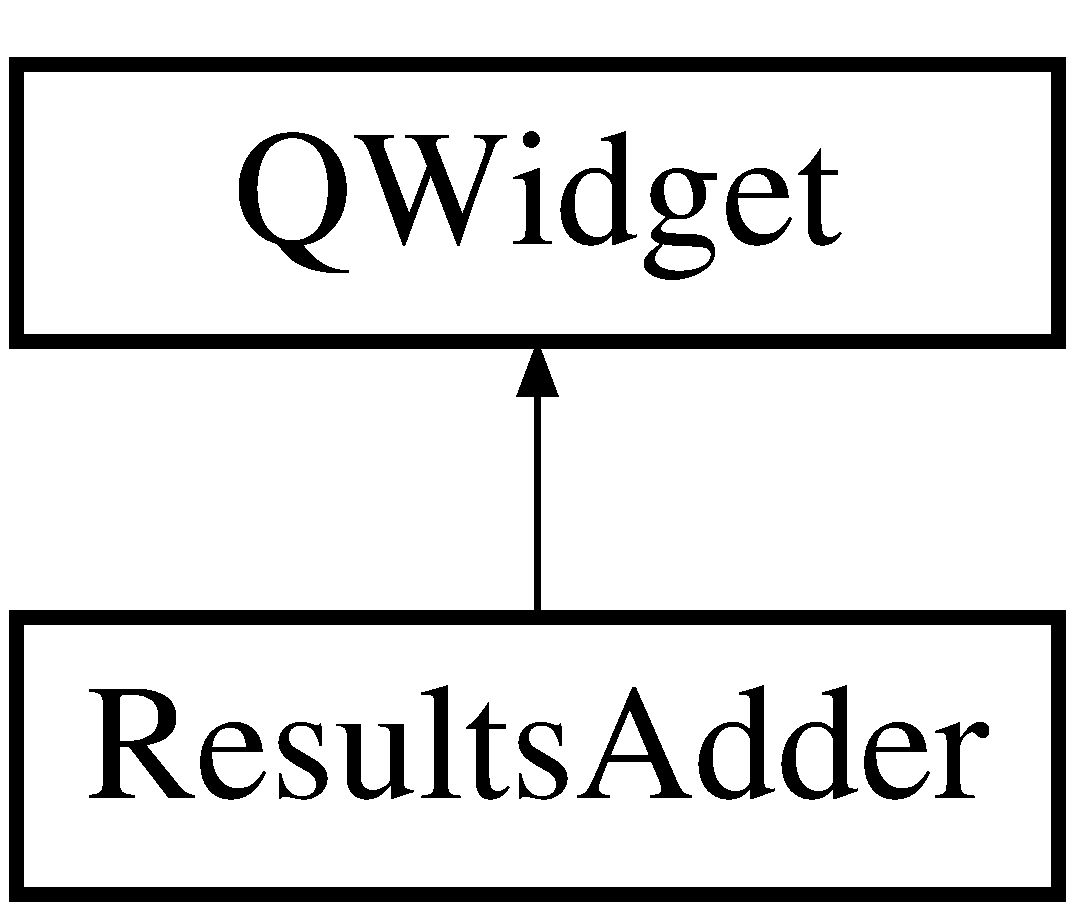
\includegraphics[height=2.000000cm]{class_results_adder}
\end{center}
\end{figure}
\subsection*{Public Slots}
\begin{DoxyCompactItemize}
\item 
void \hyperlink{class_results_adder_a97ff952c7d562a74704ca2315cb5dba2}{unlock\+Validate} ()\hypertarget{class_results_adder_a97ff952c7d562a74704ca2315cb5dba2}{}\label{class_results_adder_a97ff952c7d562a74704ca2315cb5dba2}

\begin{DoxyCompactList}\small\item\em unlock the validation button if conditions met \end{DoxyCompactList}\item 
void \hyperlink{class_results_adder_a5040ff5ce4aad855727d3f64d775fcb9}{load\+X\+ML} ()\hypertarget{class_results_adder_a5040ff5ce4aad855727d3f64d775fcb9}{}\label{class_results_adder_a5040ff5ce4aad855727d3f64d775fcb9}

\begin{DoxyCompactList}\small\item\em loads an X\+ML file into the results \end{DoxyCompactList}\item 
void \hyperlink{class_results_adder_a443573d89d5ede3de3ad88989dcd5b1e}{search\+X\+ML} ()\hypertarget{class_results_adder_a443573d89d5ede3de3ad88989dcd5b1e}{}\label{class_results_adder_a443573d89d5ede3de3ad88989dcd5b1e}

\begin{DoxyCompactList}\small\item\em browse the files to search the X\+ML result file \end{DoxyCompactList}\end{DoxyCompactItemize}
\subsection*{Public Member Functions}
\begin{DoxyCompactItemize}
\item 
{\bfseries Results\+Adder} (\hyperlink{class_image_displayer}{Image\+Displayer} $\ast$displayer, Q\+Widget $\ast$parent=0)\hypertarget{class_results_adder_aa5533172f92bb1c40af207785d6dc28f}{}\label{class_results_adder_aa5533172f92bb1c40af207785d6dc28f}

\item 
void \hyperlink{class_results_adder_af43de8c4314a87093b752734d8b70d7d}{set\+Results} (\hyperlink{class_results}{Results} $\ast$results)
\begin{DoxyCompactList}\small\item\em sets the results once they are initialized elsewhere \end{DoxyCompactList}\item 
void \hyperlink{class_results_adder_a589bc3490ffb9d11ac077cdc97bc8be2}{unlock} ()\hypertarget{class_results_adder_a589bc3490ffb9d11ac077cdc97bc8be2}{}\label{class_results_adder_a589bc3490ffb9d11ac077cdc97bc8be2}

\begin{DoxyCompactList}\small\item\em unlocks this widget \end{DoxyCompactList}\end{DoxyCompactItemize}


\subsection{Detailed Description}
A widget to add some results of detection to a results container with a G\+UI. 

\subsection{Member Function Documentation}
\index{Results\+Adder@{Results\+Adder}!set\+Results@{set\+Results}}
\index{set\+Results@{set\+Results}!Results\+Adder@{Results\+Adder}}
\subsubsection[{\texorpdfstring{set\+Results(\+Results $\ast$results)}{setResults(Results *results)}}]{\setlength{\rightskip}{0pt plus 5cm}void Results\+Adder\+::set\+Results (
\begin{DoxyParamCaption}
\item[{{\bf Results} $\ast$}]{results}
\end{DoxyParamCaption}
)}\hypertarget{class_results_adder_af43de8c4314a87093b752734d8b70d7d}{}\label{class_results_adder_af43de8c4314a87093b752734d8b70d7d}


sets the results once they are initialized elsewhere 


\begin{DoxyParams}{Parameters}
{\em results} & the initialized results \\
\hline
\end{DoxyParams}


The documentation for this class was generated from the following files\+:\begin{DoxyCompactItemize}
\item 
resultsadder.\+h\item 
resultsadder.\+cpp\end{DoxyCompactItemize}

\hypertarget{class_result_set}{}\section{Result\+Set Class Reference}
\label{class_result_set}\index{Result\+Set@{Result\+Set}}


A results set holds the results of a detection with py-\/faster-\/rcnn in one picture, the results can be from multiple model operations.  




{\ttfamily \#include $<$resultset.\+h$>$}

\subsection*{Public Member Functions}
\begin{DoxyCompactItemize}
\item 
\hyperlink{class_result_set_a9069cabfa19771579b8d3208729b426c}{Result\+Set} (std\+::string file\+Name)
\begin{DoxyCompactList}\small\item\em Builds a \hyperlink{class_result_set}{Result\+Set}. \end{DoxyCompactList}\item 
void \hyperlink{class_result_set_ad83bc3196f7a0c7e2052ad85a69c1cd3}{add\+Results} (std\+::string model\+Name, std\+::vector$<$ \hyperlink{class_object}{Object} $>$ results)
\begin{DoxyCompactList}\small\item\em adds results of a detection on this picture \end{DoxyCompactList}\item 
std\+::string \hyperlink{class_result_set_ac7ad652b95be850898dcfdcbc1c58261}{get\+File\+Name} () const 
\begin{DoxyCompactList}\small\item\em getter file\+Name \end{DoxyCompactList}\item 
std\+::vector$<$ \hyperlink{class_object}{Object} $>$ \hyperlink{class_result_set_a7f6c7ba55828add8fb3d1faf64ee8496}{objects} (std\+::string model\+Name) const 
\begin{DoxyCompactList}\small\item\em gives the detected objects by a given model \end{DoxyCompactList}\item 
std\+::vector$<$ std\+::string $>$ \hyperlink{class_result_set_a359649ed63e374f3bbba226bfeee67be}{model\+Names} () const 
\begin{DoxyCompactList}\small\item\em gets all the model names \end{DoxyCompactList}\end{DoxyCompactItemize}


\subsection{Detailed Description}
A results set holds the results of a detection with py-\/faster-\/rcnn in one picture, the results can be from multiple model operations. 

\subsection{Constructor \& Destructor Documentation}
\index{Result\+Set@{Result\+Set}!Result\+Set@{Result\+Set}}
\index{Result\+Set@{Result\+Set}!Result\+Set@{Result\+Set}}
\subsubsection[{\texorpdfstring{Result\+Set(std\+::string file\+Name)}{ResultSet(std::string fileName)}}]{\setlength{\rightskip}{0pt plus 5cm}Result\+Set\+::\+Result\+Set (
\begin{DoxyParamCaption}
\item[{std\+::string}]{file\+Name}
\end{DoxyParamCaption}
)}\hypertarget{class_result_set_a9069cabfa19771579b8d3208729b426c}{}\label{class_result_set_a9069cabfa19771579b8d3208729b426c}


Builds a \hyperlink{class_result_set}{Result\+Set}. 


\begin{DoxyParams}{Parameters}
{\em file\+Name} & the file name of the picture where the detection has been launched \\
\hline
\end{DoxyParams}


\subsection{Member Function Documentation}
\index{Result\+Set@{Result\+Set}!add\+Results@{add\+Results}}
\index{add\+Results@{add\+Results}!Result\+Set@{Result\+Set}}
\subsubsection[{\texorpdfstring{add\+Results(std\+::string model\+Name, std\+::vector$<$ Object $>$ results)}{addResults(std::string modelName, std::vector< Object > results)}}]{\setlength{\rightskip}{0pt plus 5cm}void Result\+Set\+::add\+Results (
\begin{DoxyParamCaption}
\item[{std\+::string}]{model\+Name, }
\item[{std\+::vector$<$ {\bf Object} $>$}]{results}
\end{DoxyParamCaption}
)}\hypertarget{class_result_set_ad83bc3196f7a0c7e2052ad85a69c1cd3}{}\label{class_result_set_ad83bc3196f7a0c7e2052ad85a69c1cd3}


adds results of a detection on this picture 


\begin{DoxyParams}{Parameters}
{\em model\+Name} & the name of the model that produced the detections \\
\hline
{\em results} & the objects detected \\
\hline
\end{DoxyParams}
\index{Result\+Set@{Result\+Set}!get\+File\+Name@{get\+File\+Name}}
\index{get\+File\+Name@{get\+File\+Name}!Result\+Set@{Result\+Set}}
\subsubsection[{\texorpdfstring{get\+File\+Name() const }{getFileName() const }}]{\setlength{\rightskip}{0pt plus 5cm}string Result\+Set\+::get\+File\+Name (
\begin{DoxyParamCaption}
{}
\end{DoxyParamCaption}
) const}\hypertarget{class_result_set_ac7ad652b95be850898dcfdcbc1c58261}{}\label{class_result_set_ac7ad652b95be850898dcfdcbc1c58261}


getter file\+Name 

\begin{DoxyReturn}{Returns}
a string 
\end{DoxyReturn}
\index{Result\+Set@{Result\+Set}!model\+Names@{model\+Names}}
\index{model\+Names@{model\+Names}!Result\+Set@{Result\+Set}}
\subsubsection[{\texorpdfstring{model\+Names() const }{modelNames() const }}]{\setlength{\rightskip}{0pt plus 5cm}std\+::vector$<$ string $>$ Result\+Set\+::model\+Names (
\begin{DoxyParamCaption}
{}
\end{DoxyParamCaption}
) const}\hypertarget{class_result_set_a359649ed63e374f3bbba226bfeee67be}{}\label{class_result_set_a359649ed63e374f3bbba226bfeee67be}


gets all the model names 

\begin{DoxyReturn}{Returns}
a vector of strings 
\end{DoxyReturn}
\index{Result\+Set@{Result\+Set}!objects@{objects}}
\index{objects@{objects}!Result\+Set@{Result\+Set}}
\subsubsection[{\texorpdfstring{objects(std\+::string model\+Name) const }{objects(std::string modelName) const }}]{\setlength{\rightskip}{0pt plus 5cm}std\+::vector$<$ {\bf Object} $>$ Result\+Set\+::objects (
\begin{DoxyParamCaption}
\item[{std\+::string}]{model\+Name}
\end{DoxyParamCaption}
) const}\hypertarget{class_result_set_a7f6c7ba55828add8fb3d1faf64ee8496}{}\label{class_result_set_a7f6c7ba55828add8fb3d1faf64ee8496}


gives the detected objects by a given model 


\begin{DoxyParams}{Parameters}
{\em model\+Name} & th ename of the model \\
\hline
\end{DoxyParams}
\begin{DoxyReturn}{Returns}
a vector of objects 
\end{DoxyReturn}


The documentation for this class was generated from the following files\+:\begin{DoxyCompactItemize}
\item 
resultset.\+h\item 
resultset.\+cpp\end{DoxyCompactItemize}

\hypertarget{classtinyxml2_1_1_str_pair}{}\section{tinyxml2\+:\+:Str\+Pair Class Reference}
\label{classtinyxml2_1_1_str_pair}\index{tinyxml2\+::\+Str\+Pair@{tinyxml2\+::\+Str\+Pair}}
\subsection*{Public Types}
\begin{DoxyCompactItemize}
\item 
enum \{ \\*
{\bfseries N\+E\+E\+D\+S\+\_\+\+E\+N\+T\+I\+T\+Y\+\_\+\+P\+R\+O\+C\+E\+S\+S\+I\+NG} = 0x01, 
{\bfseries N\+E\+E\+D\+S\+\_\+\+N\+E\+W\+L\+I\+N\+E\+\_\+\+N\+O\+R\+M\+A\+L\+I\+Z\+A\+T\+I\+ON} = 0x02, 
{\bfseries N\+E\+E\+D\+S\+\_\+\+W\+H\+I\+T\+E\+S\+P\+A\+C\+E\+\_\+\+C\+O\+L\+L\+A\+P\+S\+I\+NG} = 0x04, 
{\bfseries T\+E\+X\+T\+\_\+\+E\+L\+E\+M\+E\+NT} = N\+E\+E\+D\+S\+\_\+\+E\+N\+T\+I\+T\+Y\+\_\+\+P\+R\+O\+C\+E\+S\+S\+I\+NG $\vert$ N\+E\+E\+D\+S\+\_\+\+N\+E\+W\+L\+I\+N\+E\+\_\+\+N\+O\+R\+M\+A\+L\+I\+Z\+A\+T\+I\+ON, 
\\*
{\bfseries T\+E\+X\+T\+\_\+\+E\+L\+E\+M\+E\+N\+T\+\_\+\+L\+E\+A\+V\+E\+\_\+\+E\+N\+T\+I\+T\+I\+ES} = N\+E\+E\+D\+S\+\_\+\+N\+E\+W\+L\+I\+N\+E\+\_\+\+N\+O\+R\+M\+A\+L\+I\+Z\+A\+T\+I\+ON, 
{\bfseries A\+T\+T\+R\+I\+B\+U\+T\+E\+\_\+\+N\+A\+ME} = 0, 
{\bfseries A\+T\+T\+R\+I\+B\+U\+T\+E\+\_\+\+V\+A\+L\+UE} = N\+E\+E\+D\+S\+\_\+\+E\+N\+T\+I\+T\+Y\+\_\+\+P\+R\+O\+C\+E\+S\+S\+I\+NG $\vert$ N\+E\+E\+D\+S\+\_\+\+N\+E\+W\+L\+I\+N\+E\+\_\+\+N\+O\+R\+M\+A\+L\+I\+Z\+A\+T\+I\+ON, 
{\bfseries A\+T\+T\+R\+I\+B\+U\+T\+E\+\_\+\+V\+A\+L\+U\+E\+\_\+\+L\+E\+A\+V\+E\+\_\+\+E\+N\+T\+I\+T\+I\+ES} = N\+E\+E\+D\+S\+\_\+\+N\+E\+W\+L\+I\+N\+E\+\_\+\+N\+O\+R\+M\+A\+L\+I\+Z\+A\+T\+I\+ON, 
\\*
{\bfseries C\+O\+M\+M\+E\+NT} = N\+E\+E\+D\+S\+\_\+\+N\+E\+W\+L\+I\+N\+E\+\_\+\+N\+O\+R\+M\+A\+L\+I\+Z\+A\+T\+I\+ON
 \}\hypertarget{classtinyxml2_1_1_str_pair_a0301ef962e15dd94574431f1c61266c5}{}\label{classtinyxml2_1_1_str_pair_a0301ef962e15dd94574431f1c61266c5}

\end{DoxyCompactItemize}
\subsection*{Public Member Functions}
\begin{DoxyCompactItemize}
\item 
void {\bfseries Set} (char $\ast$start, char $\ast$end, int flags)\hypertarget{classtinyxml2_1_1_str_pair_a4f05549373394266a1eecba26813c166}{}\label{classtinyxml2_1_1_str_pair_a4f05549373394266a1eecba26813c166}

\item 
const char $\ast$ {\bfseries Get\+Str} ()\hypertarget{classtinyxml2_1_1_str_pair_ad87e3d11330f5e689ba1e7e54c023b57}{}\label{classtinyxml2_1_1_str_pair_ad87e3d11330f5e689ba1e7e54c023b57}

\item 
bool {\bfseries Empty} () const \hypertarget{classtinyxml2_1_1_str_pair_affa1043e73a18f05d5d2faec055725a7}{}\label{classtinyxml2_1_1_str_pair_affa1043e73a18f05d5d2faec055725a7}

\item 
void {\bfseries Set\+Interned\+Str} (const char $\ast$str)\hypertarget{classtinyxml2_1_1_str_pair_a2baf6230e18333e02ab65d0897ee3941}{}\label{classtinyxml2_1_1_str_pair_a2baf6230e18333e02ab65d0897ee3941}

\item 
void {\bfseries Set\+Str} (const char $\ast$str, int flags=0)\hypertarget{classtinyxml2_1_1_str_pair_a1f82ec6b5bee35ee7466d8565e43b1de}{}\label{classtinyxml2_1_1_str_pair_a1f82ec6b5bee35ee7466d8565e43b1de}

\item 
char $\ast$ {\bfseries Parse\+Text} (char $\ast$in, const char $\ast$end\+Tag, int str\+Flags)\hypertarget{classtinyxml2_1_1_str_pair_ad90521f188e9606a8fbafe5d86fb2246}{}\label{classtinyxml2_1_1_str_pair_ad90521f188e9606a8fbafe5d86fb2246}

\item 
char $\ast$ {\bfseries Parse\+Name} (char $\ast$in)\hypertarget{classtinyxml2_1_1_str_pair_aa6d8998efceba41d87ec2300c70a6085}{}\label{classtinyxml2_1_1_str_pair_aa6d8998efceba41d87ec2300c70a6085}

\item 
void {\bfseries Transfer\+To} (\hyperlink{classtinyxml2_1_1_str_pair}{Str\+Pair} $\ast$other)\hypertarget{classtinyxml2_1_1_str_pair_a35f795b1557fe5fdcbd93d3cc5d6b939}{}\label{classtinyxml2_1_1_str_pair_a35f795b1557fe5fdcbd93d3cc5d6b939}

\end{DoxyCompactItemize}


The documentation for this class was generated from the following files\+:\begin{DoxyCompactItemize}
\item 
src/tinyxml2.\+h\item 
src/tinyxml2.\+cpp\end{DoxyCompactItemize}

\hypertarget{classtinyxml2_1_1_x_m_l_attribute}{}\section{tinyxml2\+:\+:X\+M\+L\+Attribute Class Reference}
\label{classtinyxml2_1_1_x_m_l_attribute}\index{tinyxml2\+::\+X\+M\+L\+Attribute@{tinyxml2\+::\+X\+M\+L\+Attribute}}


{\ttfamily \#include $<$tinyxml2.\+h$>$}

\subsection*{Public Member Functions}
\begin{DoxyCompactItemize}
\item 
const char $\ast$ \hyperlink{classtinyxml2_1_1_x_m_l_attribute_a8124fbfd27f57150cc68d8a9207078c3}{Name} () const \hypertarget{classtinyxml2_1_1_x_m_l_attribute_a8124fbfd27f57150cc68d8a9207078c3}{}\label{classtinyxml2_1_1_x_m_l_attribute_a8124fbfd27f57150cc68d8a9207078c3}

\begin{DoxyCompactList}\small\item\em The name of the attribute. \end{DoxyCompactList}\item 
const char $\ast$ \hyperlink{classtinyxml2_1_1_x_m_l_attribute_aa9b08c6e592b0c88117c46666dcc1af2}{Value} () const \hypertarget{classtinyxml2_1_1_x_m_l_attribute_aa9b08c6e592b0c88117c46666dcc1af2}{}\label{classtinyxml2_1_1_x_m_l_attribute_aa9b08c6e592b0c88117c46666dcc1af2}

\begin{DoxyCompactList}\small\item\em The value of the attribute. \end{DoxyCompactList}\item 
const \hyperlink{classtinyxml2_1_1_x_m_l_attribute}{X\+M\+L\+Attribute} $\ast$ \hyperlink{classtinyxml2_1_1_x_m_l_attribute_a7fd852d6185af90361ec1bc9a7681ad6}{Next} () const \hypertarget{classtinyxml2_1_1_x_m_l_attribute_a7fd852d6185af90361ec1bc9a7681ad6}{}\label{classtinyxml2_1_1_x_m_l_attribute_a7fd852d6185af90361ec1bc9a7681ad6}

\begin{DoxyCompactList}\small\item\em The next attribute in the list. \end{DoxyCompactList}\item 
int \hyperlink{classtinyxml2_1_1_x_m_l_attribute_a949d02a5888092cc68c1e29185301863}{Int\+Value} () const 
\item 
unsigned \hyperlink{classtinyxml2_1_1_x_m_l_attribute_a4c7a179907836a136d1ce5acbe53389d}{Unsigned\+Value} () const \hypertarget{classtinyxml2_1_1_x_m_l_attribute_a4c7a179907836a136d1ce5acbe53389d}{}\label{classtinyxml2_1_1_x_m_l_attribute_a4c7a179907836a136d1ce5acbe53389d}

\begin{DoxyCompactList}\small\item\em Query as an unsigned integer. See \hyperlink{classtinyxml2_1_1_x_m_l_attribute_a949d02a5888092cc68c1e29185301863}{Int\+Value()} \end{DoxyCompactList}\item 
bool \hyperlink{classtinyxml2_1_1_x_m_l_attribute_afb444b7a12527f836aa161b54b2f7ce7}{Bool\+Value} () const \hypertarget{classtinyxml2_1_1_x_m_l_attribute_afb444b7a12527f836aa161b54b2f7ce7}{}\label{classtinyxml2_1_1_x_m_l_attribute_afb444b7a12527f836aa161b54b2f7ce7}

\begin{DoxyCompactList}\small\item\em Query as a boolean. See \hyperlink{classtinyxml2_1_1_x_m_l_attribute_a949d02a5888092cc68c1e29185301863}{Int\+Value()} \end{DoxyCompactList}\item 
double \hyperlink{classtinyxml2_1_1_x_m_l_attribute_a336153e5aa1b7ccd6502fc249bfb3fd7}{Double\+Value} () const \hypertarget{classtinyxml2_1_1_x_m_l_attribute_a336153e5aa1b7ccd6502fc249bfb3fd7}{}\label{classtinyxml2_1_1_x_m_l_attribute_a336153e5aa1b7ccd6502fc249bfb3fd7}

\begin{DoxyCompactList}\small\item\em Query as a double. See \hyperlink{classtinyxml2_1_1_x_m_l_attribute_a949d02a5888092cc68c1e29185301863}{Int\+Value()} \end{DoxyCompactList}\item 
float \hyperlink{classtinyxml2_1_1_x_m_l_attribute_ae3d51ff98eacc1dc46efcfdaee5c84ad}{Float\+Value} () const \hypertarget{classtinyxml2_1_1_x_m_l_attribute_ae3d51ff98eacc1dc46efcfdaee5c84ad}{}\label{classtinyxml2_1_1_x_m_l_attribute_ae3d51ff98eacc1dc46efcfdaee5c84ad}

\begin{DoxyCompactList}\small\item\em Query as a float. See \hyperlink{classtinyxml2_1_1_x_m_l_attribute_a949d02a5888092cc68c1e29185301863}{Int\+Value()} \end{DoxyCompactList}\item 
X\+M\+L\+Error \hyperlink{classtinyxml2_1_1_x_m_l_attribute_ad510a83c4ff2755844bb250b125d28ff}{Query\+Int\+Value} (int $\ast$value) const 
\item 
X\+M\+L\+Error \hyperlink{classtinyxml2_1_1_x_m_l_attribute_ac93f5981adfd62ac4ea76bfa668ee2b4}{Query\+Unsigned\+Value} (unsigned int $\ast$value) const \hypertarget{classtinyxml2_1_1_x_m_l_attribute_ac93f5981adfd62ac4ea76bfa668ee2b4}{}\label{classtinyxml2_1_1_x_m_l_attribute_ac93f5981adfd62ac4ea76bfa668ee2b4}

\begin{DoxyCompactList}\small\item\em See Query\+Int\+Value. \end{DoxyCompactList}\item 
X\+M\+L\+Error \hyperlink{classtinyxml2_1_1_x_m_l_attribute_a9e9b94369f182df72aaac9acd04afead}{Query\+Bool\+Value} (bool $\ast$value) const \hypertarget{classtinyxml2_1_1_x_m_l_attribute_a9e9b94369f182df72aaac9acd04afead}{}\label{classtinyxml2_1_1_x_m_l_attribute_a9e9b94369f182df72aaac9acd04afead}

\begin{DoxyCompactList}\small\item\em See Query\+Int\+Value. \end{DoxyCompactList}\item 
X\+M\+L\+Error \hyperlink{classtinyxml2_1_1_x_m_l_attribute_a0872c05edea2a7cde4bd96c1e9cb2fc4}{Query\+Double\+Value} (double $\ast$value) const \hypertarget{classtinyxml2_1_1_x_m_l_attribute_a0872c05edea2a7cde4bd96c1e9cb2fc4}{}\label{classtinyxml2_1_1_x_m_l_attribute_a0872c05edea2a7cde4bd96c1e9cb2fc4}

\begin{DoxyCompactList}\small\item\em See Query\+Int\+Value. \end{DoxyCompactList}\item 
X\+M\+L\+Error \hyperlink{classtinyxml2_1_1_x_m_l_attribute_afb254627c296d1d70b755397d32fece8}{Query\+Float\+Value} (float $\ast$value) const \hypertarget{classtinyxml2_1_1_x_m_l_attribute_afb254627c296d1d70b755397d32fece8}{}\label{classtinyxml2_1_1_x_m_l_attribute_afb254627c296d1d70b755397d32fece8}

\begin{DoxyCompactList}\small\item\em See Query\+Int\+Value. \end{DoxyCompactList}\item 
void \hyperlink{classtinyxml2_1_1_x_m_l_attribute_a406d2c4a13c7af99a65edb59dd9f7581}{Set\+Attribute} (const char $\ast$value)\hypertarget{classtinyxml2_1_1_x_m_l_attribute_a406d2c4a13c7af99a65edb59dd9f7581}{}\label{classtinyxml2_1_1_x_m_l_attribute_a406d2c4a13c7af99a65edb59dd9f7581}

\begin{DoxyCompactList}\small\item\em Set the attribute to a string value. \end{DoxyCompactList}\item 
void \hyperlink{classtinyxml2_1_1_x_m_l_attribute_ad86d7d7058d76761c3a80662566a57e5}{Set\+Attribute} (int value)\hypertarget{classtinyxml2_1_1_x_m_l_attribute_ad86d7d7058d76761c3a80662566a57e5}{}\label{classtinyxml2_1_1_x_m_l_attribute_ad86d7d7058d76761c3a80662566a57e5}

\begin{DoxyCompactList}\small\item\em Set the attribute to value. \end{DoxyCompactList}\item 
void \hyperlink{classtinyxml2_1_1_x_m_l_attribute_ae70468c0f6df2748ba3529c716999fae}{Set\+Attribute} (unsigned value)\hypertarget{classtinyxml2_1_1_x_m_l_attribute_ae70468c0f6df2748ba3529c716999fae}{}\label{classtinyxml2_1_1_x_m_l_attribute_ae70468c0f6df2748ba3529c716999fae}

\begin{DoxyCompactList}\small\item\em Set the attribute to value. \end{DoxyCompactList}\item 
void \hyperlink{classtinyxml2_1_1_x_m_l_attribute_ab3516def4fe058fe328f2b89fc2d77da}{Set\+Attribute} (bool value)\hypertarget{classtinyxml2_1_1_x_m_l_attribute_ab3516def4fe058fe328f2b89fc2d77da}{}\label{classtinyxml2_1_1_x_m_l_attribute_ab3516def4fe058fe328f2b89fc2d77da}

\begin{DoxyCompactList}\small\item\em Set the attribute to value. \end{DoxyCompactList}\item 
void \hyperlink{classtinyxml2_1_1_x_m_l_attribute_a9a65ab3147abe8ccbbd373ce8791e818}{Set\+Attribute} (double value)\hypertarget{classtinyxml2_1_1_x_m_l_attribute_a9a65ab3147abe8ccbbd373ce8791e818}{}\label{classtinyxml2_1_1_x_m_l_attribute_a9a65ab3147abe8ccbbd373ce8791e818}

\begin{DoxyCompactList}\small\item\em Set the attribute to value. \end{DoxyCompactList}\item 
void \hyperlink{classtinyxml2_1_1_x_m_l_attribute_ae95e843313aaf5d56c32530b6456df02}{Set\+Attribute} (float value)\hypertarget{classtinyxml2_1_1_x_m_l_attribute_ae95e843313aaf5d56c32530b6456df02}{}\label{classtinyxml2_1_1_x_m_l_attribute_ae95e843313aaf5d56c32530b6456df02}

\begin{DoxyCompactList}\small\item\em Set the attribute to value. \end{DoxyCompactList}\end{DoxyCompactItemize}
\subsection*{Friends}
\begin{DoxyCompactItemize}
\item 
class {\bfseries X\+M\+L\+Element}\hypertarget{classtinyxml2_1_1_x_m_l_attribute_ac2fba9b6e452829dd892f7392c24e0eb}{}\label{classtinyxml2_1_1_x_m_l_attribute_ac2fba9b6e452829dd892f7392c24e0eb}

\end{DoxyCompactItemize}


\subsection{Detailed Description}
An attribute is a name-\/value pair. Elements have an arbitrary number of attributes, each with a unique name.

\begin{DoxyNote}{Note}
The attributes are not X\+M\+L\+Nodes. You may only query the \hyperlink{classtinyxml2_1_1_x_m_l_attribute_a7fd852d6185af90361ec1bc9a7681ad6}{Next()} attribute in a list. 
\end{DoxyNote}


\subsection{Member Function Documentation}
\index{tinyxml2\+::\+X\+M\+L\+Attribute@{tinyxml2\+::\+X\+M\+L\+Attribute}!Int\+Value@{Int\+Value}}
\index{Int\+Value@{Int\+Value}!tinyxml2\+::\+X\+M\+L\+Attribute@{tinyxml2\+::\+X\+M\+L\+Attribute}}
\subsubsection[{\texorpdfstring{Int\+Value() const }{IntValue() const }}]{\setlength{\rightskip}{0pt plus 5cm}int tinyxml2\+::\+X\+M\+L\+Attribute\+::\+Int\+Value (
\begin{DoxyParamCaption}
{}
\end{DoxyParamCaption}
) const\hspace{0.3cm}{\ttfamily [inline]}}\hypertarget{classtinyxml2_1_1_x_m_l_attribute_a949d02a5888092cc68c1e29185301863}{}\label{classtinyxml2_1_1_x_m_l_attribute_a949d02a5888092cc68c1e29185301863}
Int\+Value interprets the attribute as an integer, and returns the value. If the value isn\textquotesingle{}t an integer, 0 will be returned. There is no error checking; use \hyperlink{classtinyxml2_1_1_x_m_l_attribute_ad510a83c4ff2755844bb250b125d28ff}{Query\+Int\+Value()} if you need error checking. \index{tinyxml2\+::\+X\+M\+L\+Attribute@{tinyxml2\+::\+X\+M\+L\+Attribute}!Query\+Int\+Value@{Query\+Int\+Value}}
\index{Query\+Int\+Value@{Query\+Int\+Value}!tinyxml2\+::\+X\+M\+L\+Attribute@{tinyxml2\+::\+X\+M\+L\+Attribute}}
\subsubsection[{\texorpdfstring{Query\+Int\+Value(int $\ast$value) const }{QueryIntValue(int *value) const }}]{\setlength{\rightskip}{0pt plus 5cm}X\+M\+L\+Error tinyxml2\+::\+X\+M\+L\+Attribute\+::\+Query\+Int\+Value (
\begin{DoxyParamCaption}
\item[{int $\ast$}]{value}
\end{DoxyParamCaption}
) const}\hypertarget{classtinyxml2_1_1_x_m_l_attribute_ad510a83c4ff2755844bb250b125d28ff}{}\label{classtinyxml2_1_1_x_m_l_attribute_ad510a83c4ff2755844bb250b125d28ff}
Query\+Int\+Value interprets the attribute as an integer, and returns the value in the provided parameter. The function will return X\+M\+L\+\_\+\+N\+O\+\_\+\+E\+R\+R\+OR on success, and X\+M\+L\+\_\+\+W\+R\+O\+N\+G\+\_\+\+A\+T\+T\+R\+I\+B\+U\+T\+E\+\_\+\+T\+Y\+PE if the conversion is not successful. 

The documentation for this class was generated from the following files\+:\begin{DoxyCompactItemize}
\item 
src/tinyxml2.\+h\item 
src/tinyxml2.\+cpp\end{DoxyCompactItemize}

\hypertarget{classtinyxml2_1_1_x_m_l_comment}{}\section{tinyxml2\+:\+:X\+M\+L\+Comment Class Reference}
\label{classtinyxml2_1_1_x_m_l_comment}\index{tinyxml2\+::\+X\+M\+L\+Comment@{tinyxml2\+::\+X\+M\+L\+Comment}}


{\ttfamily \#include $<$tinyxml2.\+h$>$}

Inheritance diagram for tinyxml2\+:\+:X\+M\+L\+Comment\+:\begin{figure}[H]
\begin{center}
\leavevmode
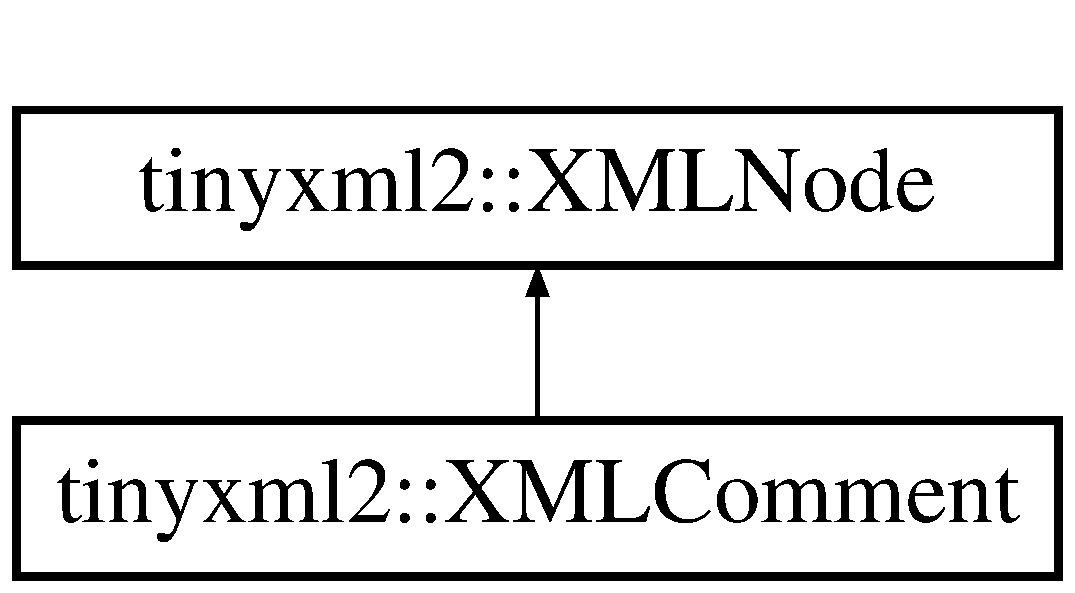
\includegraphics[height=2.000000cm]{classtinyxml2_1_1_x_m_l_comment}
\end{center}
\end{figure}
\subsection*{Public Member Functions}
\begin{DoxyCompactItemize}
\item 
virtual \hyperlink{classtinyxml2_1_1_x_m_l_comment}{X\+M\+L\+Comment} $\ast$ \hyperlink{classtinyxml2_1_1_x_m_l_comment_a8093e1dc8a34fa446d9dc3fde0e6c0ee}{To\+Comment} ()\hypertarget{classtinyxml2_1_1_x_m_l_comment_a8093e1dc8a34fa446d9dc3fde0e6c0ee}{}\label{classtinyxml2_1_1_x_m_l_comment_a8093e1dc8a34fa446d9dc3fde0e6c0ee}

\begin{DoxyCompactList}\small\item\em Safely cast to a Comment, or null. \end{DoxyCompactList}\item 
virtual const \hyperlink{classtinyxml2_1_1_x_m_l_comment}{X\+M\+L\+Comment} $\ast$ {\bfseries To\+Comment} () const \hypertarget{classtinyxml2_1_1_x_m_l_comment_a422aabac22de7d9c9cad130897dd8b1c}{}\label{classtinyxml2_1_1_x_m_l_comment_a422aabac22de7d9c9cad130897dd8b1c}

\item 
virtual bool \hyperlink{classtinyxml2_1_1_x_m_l_comment_aa382b1be6a8b0650c16a2d88bb499335}{Accept} (\hyperlink{classtinyxml2_1_1_x_m_l_visitor}{X\+M\+L\+Visitor} $\ast$visitor) const 
\item 
virtual \hyperlink{classtinyxml2_1_1_x_m_l_node}{X\+M\+L\+Node} $\ast$ \hyperlink{classtinyxml2_1_1_x_m_l_comment_a90bb60193a691b484f5e1b487857016d}{Shallow\+Clone} (\hyperlink{classtinyxml2_1_1_x_m_l_document}{X\+M\+L\+Document} $\ast$document) const 
\item 
virtual bool \hyperlink{classtinyxml2_1_1_x_m_l_comment_a2d9f26757b0018fce933e74420cda22a}{Shallow\+Equal} (const \hyperlink{classtinyxml2_1_1_x_m_l_node}{X\+M\+L\+Node} $\ast$compare) const 
\end{DoxyCompactItemize}
\subsection*{Protected Member Functions}
\begin{DoxyCompactItemize}
\item 
{\bfseries X\+M\+L\+Comment} (\hyperlink{classtinyxml2_1_1_x_m_l_document}{X\+M\+L\+Document} $\ast$doc)\hypertarget{classtinyxml2_1_1_x_m_l_comment_ae6463adc3edd93a8e5a9b2b7e99cdf91}{}\label{classtinyxml2_1_1_x_m_l_comment_ae6463adc3edd93a8e5a9b2b7e99cdf91}

\item 
char $\ast$ {\bfseries Parse\+Deep} (char $\ast$, \hyperlink{classtinyxml2_1_1_str_pair}{Str\+Pair} $\ast$end\+Tag)\hypertarget{classtinyxml2_1_1_x_m_l_comment_aa6ab35c3bb1c1840371dc32a2040c57f}{}\label{classtinyxml2_1_1_x_m_l_comment_aa6ab35c3bb1c1840371dc32a2040c57f}

\end{DoxyCompactItemize}
\subsection*{Friends}
\begin{DoxyCompactItemize}
\item 
class {\bfseries X\+M\+L\+Document}\hypertarget{classtinyxml2_1_1_x_m_l_comment_a4eee3bda60c60a30e4e8cd4ea91c4c6e}{}\label{classtinyxml2_1_1_x_m_l_comment_a4eee3bda60c60a30e4e8cd4ea91c4c6e}

\end{DoxyCompactItemize}
\subsection*{Additional Inherited Members}


\subsection{Detailed Description}
An X\+ML Comment. 

\subsection{Member Function Documentation}
\index{tinyxml2\+::\+X\+M\+L\+Comment@{tinyxml2\+::\+X\+M\+L\+Comment}!Accept@{Accept}}
\index{Accept@{Accept}!tinyxml2\+::\+X\+M\+L\+Comment@{tinyxml2\+::\+X\+M\+L\+Comment}}
\subsubsection[{\texorpdfstring{Accept(\+X\+M\+L\+Visitor $\ast$visitor) const }{Accept(XMLVisitor *visitor) const }}]{\setlength{\rightskip}{0pt plus 5cm}bool tinyxml2\+::\+X\+M\+L\+Comment\+::\+Accept (
\begin{DoxyParamCaption}
\item[{{\bf X\+M\+L\+Visitor} $\ast$}]{visitor}
\end{DoxyParamCaption}
) const\hspace{0.3cm}{\ttfamily [virtual]}}\hypertarget{classtinyxml2_1_1_x_m_l_comment_aa382b1be6a8b0650c16a2d88bb499335}{}\label{classtinyxml2_1_1_x_m_l_comment_aa382b1be6a8b0650c16a2d88bb499335}
Accept a hierarchical visit of the nodes in the Tiny\+X\+M\+L-\/2 D\+OM. Every node in the X\+ML tree will be conditionally visited and the host will be called back via the \hyperlink{classtinyxml2_1_1_x_m_l_visitor}{X\+M\+L\+Visitor} interface.

This is essentially a S\+AX interface for Tiny\+X\+M\+L-\/2. (Note however it doesn\textquotesingle{}t re-\/parse the X\+ML for the callbacks, so the performance of Tiny\+X\+M\+L-\/2 is unchanged by using this interface versus any other.)

The interface has been based on ideas from\+:


\begin{DoxyItemize}
\item \href{http://www.saxproject.org/}{\tt http\+://www.\+saxproject.\+org/}
\item \href{http://c2.com/cgi/wiki?HierarchicalVisitorPattern}{\tt http\+://c2.\+com/cgi/wiki?\+Hierarchical\+Visitor\+Pattern}
\end{DoxyItemize}

Which are both good references for \char`\"{}visiting\char`\"{}.

An example of using \hyperlink{classtinyxml2_1_1_x_m_l_comment_aa382b1be6a8b0650c16a2d88bb499335}{Accept()}\+: \begin{DoxyVerb}XMLPrinter printer;
tinyxmlDoc.Accept( &printer );
const char* xmlcstr = printer.CStr();
\end{DoxyVerb}
 

Implements \hyperlink{classtinyxml2_1_1_x_m_l_node_a366ad0e9b9ae8d1b18c00f903994b7a9}{tinyxml2\+::\+X\+M\+L\+Node}.

\index{tinyxml2\+::\+X\+M\+L\+Comment@{tinyxml2\+::\+X\+M\+L\+Comment}!Shallow\+Clone@{Shallow\+Clone}}
\index{Shallow\+Clone@{Shallow\+Clone}!tinyxml2\+::\+X\+M\+L\+Comment@{tinyxml2\+::\+X\+M\+L\+Comment}}
\subsubsection[{\texorpdfstring{Shallow\+Clone(\+X\+M\+L\+Document $\ast$document) const }{ShallowClone(XMLDocument *document) const }}]{\setlength{\rightskip}{0pt plus 5cm}{\bf X\+M\+L\+Node} $\ast$ tinyxml2\+::\+X\+M\+L\+Comment\+::\+Shallow\+Clone (
\begin{DoxyParamCaption}
\item[{{\bf X\+M\+L\+Document} $\ast$}]{document}
\end{DoxyParamCaption}
) const\hspace{0.3cm}{\ttfamily [virtual]}}\hypertarget{classtinyxml2_1_1_x_m_l_comment_a90bb60193a691b484f5e1b487857016d}{}\label{classtinyxml2_1_1_x_m_l_comment_a90bb60193a691b484f5e1b487857016d}
Make a copy of this node, but not its children. You may pass in a Document pointer that will be the owner of the new Node. If the \textquotesingle{}document\textquotesingle{} is null, then the node returned will be allocated from the current Document. (this-\/$>$\hyperlink{classtinyxml2_1_1_x_m_l_node_af343d1ef0b45c0020e62d784d7e67a68}{Get\+Document()})

Note\+: if called on a \hyperlink{classtinyxml2_1_1_x_m_l_document}{X\+M\+L\+Document}, this will return null. 

Implements \hyperlink{classtinyxml2_1_1_x_m_l_node_a83e3524e2ecea25eeab630c7ab113627}{tinyxml2\+::\+X\+M\+L\+Node}.

\index{tinyxml2\+::\+X\+M\+L\+Comment@{tinyxml2\+::\+X\+M\+L\+Comment}!Shallow\+Equal@{Shallow\+Equal}}
\index{Shallow\+Equal@{Shallow\+Equal}!tinyxml2\+::\+X\+M\+L\+Comment@{tinyxml2\+::\+X\+M\+L\+Comment}}
\subsubsection[{\texorpdfstring{Shallow\+Equal(const X\+M\+L\+Node $\ast$compare) const }{ShallowEqual(const XMLNode *compare) const }}]{\setlength{\rightskip}{0pt plus 5cm}bool tinyxml2\+::\+X\+M\+L\+Comment\+::\+Shallow\+Equal (
\begin{DoxyParamCaption}
\item[{const {\bf X\+M\+L\+Node} $\ast$}]{compare}
\end{DoxyParamCaption}
) const\hspace{0.3cm}{\ttfamily [virtual]}}\hypertarget{classtinyxml2_1_1_x_m_l_comment_a2d9f26757b0018fce933e74420cda22a}{}\label{classtinyxml2_1_1_x_m_l_comment_a2d9f26757b0018fce933e74420cda22a}
Test if 2 nodes are the same, but don\textquotesingle{}t test children. The 2 nodes do not need to be in the same Document.

Note\+: if called on a \hyperlink{classtinyxml2_1_1_x_m_l_document}{X\+M\+L\+Document}, this will return false. 

Implements \hyperlink{classtinyxml2_1_1_x_m_l_node_ac50408e91e095237f45716092ac2bddc}{tinyxml2\+::\+X\+M\+L\+Node}.



The documentation for this class was generated from the following files\+:\begin{DoxyCompactItemize}
\item 
tinyxml2.\+h\item 
tinyxml2.\+cpp\end{DoxyCompactItemize}

\hypertarget{classtinyxml2_1_1_x_m_l_const_handle}{}\section{tinyxml2\+:\+:X\+M\+L\+Const\+Handle Class Reference}
\label{classtinyxml2_1_1_x_m_l_const_handle}\index{tinyxml2\+::\+X\+M\+L\+Const\+Handle@{tinyxml2\+::\+X\+M\+L\+Const\+Handle}}


{\ttfamily \#include $<$tinyxml2.\+h$>$}

\subsection*{Public Member Functions}
\begin{DoxyCompactItemize}
\item 
{\bfseries X\+M\+L\+Const\+Handle} (const \hyperlink{classtinyxml2_1_1_x_m_l_node}{X\+M\+L\+Node} $\ast$node)\hypertarget{classtinyxml2_1_1_x_m_l_const_handle_a098bda71fa11d7c74ccddab59d5dd534}{}\label{classtinyxml2_1_1_x_m_l_const_handle_a098bda71fa11d7c74ccddab59d5dd534}

\item 
{\bfseries X\+M\+L\+Const\+Handle} (const \hyperlink{classtinyxml2_1_1_x_m_l_node}{X\+M\+L\+Node} \&node)\hypertarget{classtinyxml2_1_1_x_m_l_const_handle_a8420a0c4720637e0529e78c2e22f2b0b}{}\label{classtinyxml2_1_1_x_m_l_const_handle_a8420a0c4720637e0529e78c2e22f2b0b}

\item 
{\bfseries X\+M\+L\+Const\+Handle} (const \hyperlink{classtinyxml2_1_1_x_m_l_const_handle}{X\+M\+L\+Const\+Handle} \&ref)\hypertarget{classtinyxml2_1_1_x_m_l_const_handle_a639317ad315ff24f4ef0dc69312d7303}{}\label{classtinyxml2_1_1_x_m_l_const_handle_a639317ad315ff24f4ef0dc69312d7303}

\item 
\hyperlink{classtinyxml2_1_1_x_m_l_const_handle}{X\+M\+L\+Const\+Handle} \& {\bfseries operator=} (const \hyperlink{classtinyxml2_1_1_x_m_l_const_handle}{X\+M\+L\+Const\+Handle} \&ref)\hypertarget{classtinyxml2_1_1_x_m_l_const_handle_a2d74c91df1ff9aa5f9b57e3dceddbf94}{}\label{classtinyxml2_1_1_x_m_l_const_handle_a2d74c91df1ff9aa5f9b57e3dceddbf94}

\item 
const \hyperlink{classtinyxml2_1_1_x_m_l_const_handle}{X\+M\+L\+Const\+Handle} {\bfseries First\+Child} () const \hypertarget{classtinyxml2_1_1_x_m_l_const_handle_a64c4ff7074effc1fd181d68d23f9d1e4}{}\label{classtinyxml2_1_1_x_m_l_const_handle_a64c4ff7074effc1fd181d68d23f9d1e4}

\item 
const \hyperlink{classtinyxml2_1_1_x_m_l_const_handle}{X\+M\+L\+Const\+Handle} {\bfseries First\+Child\+Element} (const char $\ast$name=0) const \hypertarget{classtinyxml2_1_1_x_m_l_const_handle_a686a96a178dfb51ca9402e22b4a4cd10}{}\label{classtinyxml2_1_1_x_m_l_const_handle_a686a96a178dfb51ca9402e22b4a4cd10}

\item 
const \hyperlink{classtinyxml2_1_1_x_m_l_const_handle}{X\+M\+L\+Const\+Handle} {\bfseries Last\+Child} () const \hypertarget{classtinyxml2_1_1_x_m_l_const_handle_afec9a68e7951193bc5a6e876d602f263}{}\label{classtinyxml2_1_1_x_m_l_const_handle_afec9a68e7951193bc5a6e876d602f263}

\item 
const \hyperlink{classtinyxml2_1_1_x_m_l_const_handle}{X\+M\+L\+Const\+Handle} {\bfseries Last\+Child\+Element} (const char $\ast$name=0) const \hypertarget{classtinyxml2_1_1_x_m_l_const_handle_a8f08be56cd748bd1a756a7c57e8a4e8b}{}\label{classtinyxml2_1_1_x_m_l_const_handle_a8f08be56cd748bd1a756a7c57e8a4e8b}

\item 
const \hyperlink{classtinyxml2_1_1_x_m_l_const_handle}{X\+M\+L\+Const\+Handle} {\bfseries Previous\+Sibling} () const \hypertarget{classtinyxml2_1_1_x_m_l_const_handle_a6917564e26b2c20ebdcb23c7940ad80a}{}\label{classtinyxml2_1_1_x_m_l_const_handle_a6917564e26b2c20ebdcb23c7940ad80a}

\item 
const \hyperlink{classtinyxml2_1_1_x_m_l_const_handle}{X\+M\+L\+Const\+Handle} {\bfseries Previous\+Sibling\+Element} (const char $\ast$name=0) const \hypertarget{classtinyxml2_1_1_x_m_l_const_handle_afe1b35a9c897ae45f74e8d615cb98c2a}{}\label{classtinyxml2_1_1_x_m_l_const_handle_afe1b35a9c897ae45f74e8d615cb98c2a}

\item 
const \hyperlink{classtinyxml2_1_1_x_m_l_const_handle}{X\+M\+L\+Const\+Handle} {\bfseries Next\+Sibling} () const \hypertarget{classtinyxml2_1_1_x_m_l_const_handle_a596e248c8014d718f41658502a2e221b}{}\label{classtinyxml2_1_1_x_m_l_const_handle_a596e248c8014d718f41658502a2e221b}

\item 
const \hyperlink{classtinyxml2_1_1_x_m_l_const_handle}{X\+M\+L\+Const\+Handle} {\bfseries Next\+Sibling\+Element} (const char $\ast$name=0) const \hypertarget{classtinyxml2_1_1_x_m_l_const_handle_a0d50f71f0d4199768508f039426e2b1f}{}\label{classtinyxml2_1_1_x_m_l_const_handle_a0d50f71f0d4199768508f039426e2b1f}

\item 
const \hyperlink{classtinyxml2_1_1_x_m_l_node}{X\+M\+L\+Node} $\ast$ {\bfseries To\+Node} () const \hypertarget{classtinyxml2_1_1_x_m_l_const_handle_a95d0256318c10c3f75fa5f8ffb3e4bc1}{}\label{classtinyxml2_1_1_x_m_l_const_handle_a95d0256318c10c3f75fa5f8ffb3e4bc1}

\item 
const \hyperlink{classtinyxml2_1_1_x_m_l_element}{X\+M\+L\+Element} $\ast$ {\bfseries To\+Element} () const \hypertarget{classtinyxml2_1_1_x_m_l_const_handle_a5a48adefc2a5e70d4ce5b55692a0e2f9}{}\label{classtinyxml2_1_1_x_m_l_const_handle_a5a48adefc2a5e70d4ce5b55692a0e2f9}

\item 
const \hyperlink{classtinyxml2_1_1_x_m_l_text}{X\+M\+L\+Text} $\ast$ {\bfseries To\+Text} () const \hypertarget{classtinyxml2_1_1_x_m_l_const_handle_ad86ca7dbb20d0495ae357fe7a866e0be}{}\label{classtinyxml2_1_1_x_m_l_const_handle_ad86ca7dbb20d0495ae357fe7a866e0be}

\item 
const \hyperlink{classtinyxml2_1_1_x_m_l_unknown}{X\+M\+L\+Unknown} $\ast$ {\bfseries To\+Unknown} () const \hypertarget{classtinyxml2_1_1_x_m_l_const_handle_acb358a329e54fa204ed2d0b181566828}{}\label{classtinyxml2_1_1_x_m_l_const_handle_acb358a329e54fa204ed2d0b181566828}

\item 
const \hyperlink{classtinyxml2_1_1_x_m_l_declaration}{X\+M\+L\+Declaration} $\ast$ {\bfseries To\+Declaration} () const \hypertarget{classtinyxml2_1_1_x_m_l_const_handle_a5de0c175845bc30a6f9b3d88d8877eaf}{}\label{classtinyxml2_1_1_x_m_l_const_handle_a5de0c175845bc30a6f9b3d88d8877eaf}

\end{DoxyCompactItemize}


\subsection{Detailed Description}
A variant of the \hyperlink{classtinyxml2_1_1_x_m_l_handle}{X\+M\+L\+Handle} class for working with const X\+M\+L\+Nodes and Documents. It is the same in all regards, except for the \textquotesingle{}const\textquotesingle{} qualifiers. See \hyperlink{classtinyxml2_1_1_x_m_l_handle}{X\+M\+L\+Handle} for A\+PI. 

The documentation for this class was generated from the following file\+:\begin{DoxyCompactItemize}
\item 
tinyxml2.\+h\end{DoxyCompactItemize}

\hypertarget{classtinyxml2_1_1_x_m_l_declaration}{}\section{tinyxml2\+:\+:X\+M\+L\+Declaration Class Reference}
\label{classtinyxml2_1_1_x_m_l_declaration}\index{tinyxml2\+::\+X\+M\+L\+Declaration@{tinyxml2\+::\+X\+M\+L\+Declaration}}


{\ttfamily \#include $<$tinyxml2.\+h$>$}

Inheritance diagram for tinyxml2\+:\+:X\+M\+L\+Declaration\+:\begin{figure}[H]
\begin{center}
\leavevmode
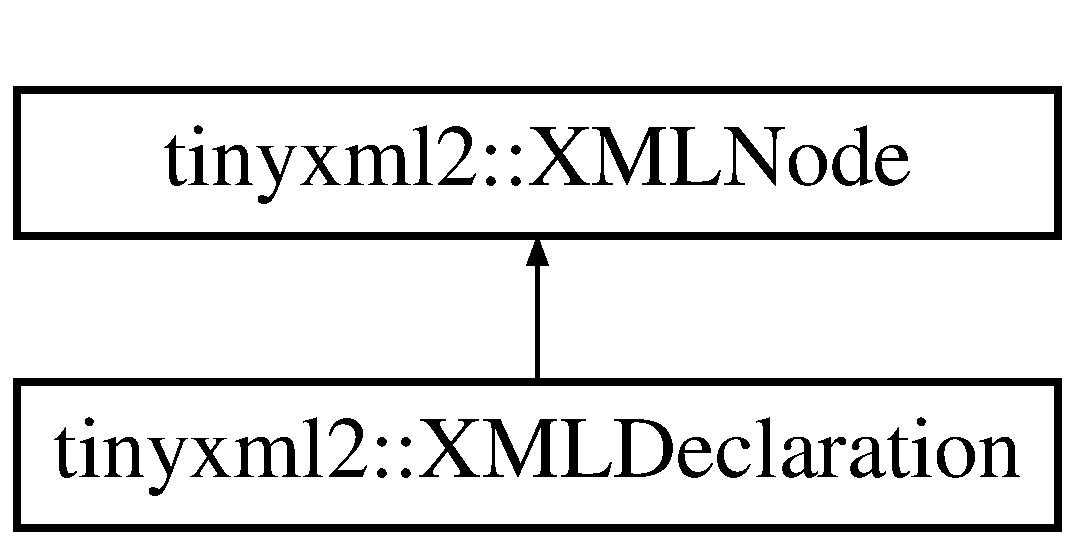
\includegraphics[height=2.000000cm]{classtinyxml2_1_1_x_m_l_declaration}
\end{center}
\end{figure}
\subsection*{Public Member Functions}
\begin{DoxyCompactItemize}
\item 
virtual \hyperlink{classtinyxml2_1_1_x_m_l_declaration}{X\+M\+L\+Declaration} $\ast$ \hyperlink{classtinyxml2_1_1_x_m_l_declaration_a159d8ac45865215e88059ea1e5b52fc5}{To\+Declaration} ()\hypertarget{classtinyxml2_1_1_x_m_l_declaration_a159d8ac45865215e88059ea1e5b52fc5}{}\label{classtinyxml2_1_1_x_m_l_declaration_a159d8ac45865215e88059ea1e5b52fc5}

\begin{DoxyCompactList}\small\item\em Safely cast to a Declaration, or null. \end{DoxyCompactList}\item 
virtual const \hyperlink{classtinyxml2_1_1_x_m_l_declaration}{X\+M\+L\+Declaration} $\ast$ {\bfseries To\+Declaration} () const \hypertarget{classtinyxml2_1_1_x_m_l_declaration_af724607a5fa810496fd6a21f5975a643}{}\label{classtinyxml2_1_1_x_m_l_declaration_af724607a5fa810496fd6a21f5975a643}

\item 
virtual bool \hyperlink{classtinyxml2_1_1_x_m_l_declaration_a953a7359cc312d15218eb5843a4ca108}{Accept} (\hyperlink{classtinyxml2_1_1_x_m_l_visitor}{X\+M\+L\+Visitor} $\ast$visitor) const 
\item 
virtual \hyperlink{classtinyxml2_1_1_x_m_l_node}{X\+M\+L\+Node} $\ast$ \hyperlink{classtinyxml2_1_1_x_m_l_declaration_a39458732ee6796cfc85dd35d3c488e0b}{Shallow\+Clone} (\hyperlink{classtinyxml2_1_1_x_m_l_document}{X\+M\+L\+Document} $\ast$document) const 
\item 
virtual bool \hyperlink{classtinyxml2_1_1_x_m_l_declaration_ace0d2d9bc1b63278bd5e984ebe0c7bd0}{Shallow\+Equal} (const \hyperlink{classtinyxml2_1_1_x_m_l_node}{X\+M\+L\+Node} $\ast$compare) const 
\end{DoxyCompactItemize}
\subsection*{Protected Member Functions}
\begin{DoxyCompactItemize}
\item 
{\bfseries X\+M\+L\+Declaration} (\hyperlink{classtinyxml2_1_1_x_m_l_document}{X\+M\+L\+Document} $\ast$doc)\hypertarget{classtinyxml2_1_1_x_m_l_declaration_aef9586f2ce5df5feba74dde49a242b06}{}\label{classtinyxml2_1_1_x_m_l_declaration_aef9586f2ce5df5feba74dde49a242b06}

\item 
char $\ast$ {\bfseries Parse\+Deep} (char $\ast$, \hyperlink{classtinyxml2_1_1_str_pair}{Str\+Pair} $\ast$end\+Tag)\hypertarget{classtinyxml2_1_1_x_m_l_declaration_a19e33e0a9f9500f449261558c36f9a44}{}\label{classtinyxml2_1_1_x_m_l_declaration_a19e33e0a9f9500f449261558c36f9a44}

\end{DoxyCompactItemize}
\subsection*{Friends}
\begin{DoxyCompactItemize}
\item 
class {\bfseries X\+M\+L\+Document}\hypertarget{classtinyxml2_1_1_x_m_l_declaration_a4eee3bda60c60a30e4e8cd4ea91c4c6e}{}\label{classtinyxml2_1_1_x_m_l_declaration_a4eee3bda60c60a30e4e8cd4ea91c4c6e}

\end{DoxyCompactItemize}
\subsection*{Additional Inherited Members}


\subsection{Detailed Description}
In correct X\+ML the declaration is the first entry in the file. \begin{DoxyVerb}    <?xml version="1.0" standalone="yes"?>
\end{DoxyVerb}


Tiny\+X\+M\+L-\/2 will happily read or write files without a declaration, however.

The text of the declaration isn\textquotesingle{}t interpreted. It is parsed and written as a string. 

\subsection{Member Function Documentation}
\index{tinyxml2\+::\+X\+M\+L\+Declaration@{tinyxml2\+::\+X\+M\+L\+Declaration}!Accept@{Accept}}
\index{Accept@{Accept}!tinyxml2\+::\+X\+M\+L\+Declaration@{tinyxml2\+::\+X\+M\+L\+Declaration}}
\subsubsection[{\texorpdfstring{Accept(\+X\+M\+L\+Visitor $\ast$visitor) const }{Accept(XMLVisitor *visitor) const }}]{\setlength{\rightskip}{0pt plus 5cm}bool tinyxml2\+::\+X\+M\+L\+Declaration\+::\+Accept (
\begin{DoxyParamCaption}
\item[{{\bf X\+M\+L\+Visitor} $\ast$}]{visitor}
\end{DoxyParamCaption}
) const\hspace{0.3cm}{\ttfamily [virtual]}}\hypertarget{classtinyxml2_1_1_x_m_l_declaration_a953a7359cc312d15218eb5843a4ca108}{}\label{classtinyxml2_1_1_x_m_l_declaration_a953a7359cc312d15218eb5843a4ca108}
Accept a hierarchical visit of the nodes in the Tiny\+X\+M\+L-\/2 D\+OM. Every node in the X\+ML tree will be conditionally visited and the host will be called back via the \hyperlink{classtinyxml2_1_1_x_m_l_visitor}{X\+M\+L\+Visitor} interface.

This is essentially a S\+AX interface for Tiny\+X\+M\+L-\/2. (Note however it doesn\textquotesingle{}t re-\/parse the X\+ML for the callbacks, so the performance of Tiny\+X\+M\+L-\/2 is unchanged by using this interface versus any other.)

The interface has been based on ideas from\+:


\begin{DoxyItemize}
\item \href{http://www.saxproject.org/}{\tt http\+://www.\+saxproject.\+org/}
\item \href{http://c2.com/cgi/wiki?HierarchicalVisitorPattern}{\tt http\+://c2.\+com/cgi/wiki?\+Hierarchical\+Visitor\+Pattern}
\end{DoxyItemize}

Which are both good references for \char`\"{}visiting\char`\"{}.

An example of using \hyperlink{classtinyxml2_1_1_x_m_l_declaration_a953a7359cc312d15218eb5843a4ca108}{Accept()}\+: \begin{DoxyVerb}XMLPrinter printer;
tinyxmlDoc.Accept( &printer );
const char* xmlcstr = printer.CStr();
\end{DoxyVerb}
 

Implements \hyperlink{classtinyxml2_1_1_x_m_l_node_a366ad0e9b9ae8d1b18c00f903994b7a9}{tinyxml2\+::\+X\+M\+L\+Node}.

\index{tinyxml2\+::\+X\+M\+L\+Declaration@{tinyxml2\+::\+X\+M\+L\+Declaration}!Shallow\+Clone@{Shallow\+Clone}}
\index{Shallow\+Clone@{Shallow\+Clone}!tinyxml2\+::\+X\+M\+L\+Declaration@{tinyxml2\+::\+X\+M\+L\+Declaration}}
\subsubsection[{\texorpdfstring{Shallow\+Clone(\+X\+M\+L\+Document $\ast$document) const }{ShallowClone(XMLDocument *document) const }}]{\setlength{\rightskip}{0pt plus 5cm}{\bf X\+M\+L\+Node} $\ast$ tinyxml2\+::\+X\+M\+L\+Declaration\+::\+Shallow\+Clone (
\begin{DoxyParamCaption}
\item[{{\bf X\+M\+L\+Document} $\ast$}]{document}
\end{DoxyParamCaption}
) const\hspace{0.3cm}{\ttfamily [virtual]}}\hypertarget{classtinyxml2_1_1_x_m_l_declaration_a39458732ee6796cfc85dd35d3c488e0b}{}\label{classtinyxml2_1_1_x_m_l_declaration_a39458732ee6796cfc85dd35d3c488e0b}
Make a copy of this node, but not its children. You may pass in a Document pointer that will be the owner of the new Node. If the \textquotesingle{}document\textquotesingle{} is null, then the node returned will be allocated from the current Document. (this-\/$>$\hyperlink{classtinyxml2_1_1_x_m_l_node_af343d1ef0b45c0020e62d784d7e67a68}{Get\+Document()})

Note\+: if called on a \hyperlink{classtinyxml2_1_1_x_m_l_document}{X\+M\+L\+Document}, this will return null. 

Implements \hyperlink{classtinyxml2_1_1_x_m_l_node_a83e3524e2ecea25eeab630c7ab113627}{tinyxml2\+::\+X\+M\+L\+Node}.

\index{tinyxml2\+::\+X\+M\+L\+Declaration@{tinyxml2\+::\+X\+M\+L\+Declaration}!Shallow\+Equal@{Shallow\+Equal}}
\index{Shallow\+Equal@{Shallow\+Equal}!tinyxml2\+::\+X\+M\+L\+Declaration@{tinyxml2\+::\+X\+M\+L\+Declaration}}
\subsubsection[{\texorpdfstring{Shallow\+Equal(const X\+M\+L\+Node $\ast$compare) const }{ShallowEqual(const XMLNode *compare) const }}]{\setlength{\rightskip}{0pt plus 5cm}bool tinyxml2\+::\+X\+M\+L\+Declaration\+::\+Shallow\+Equal (
\begin{DoxyParamCaption}
\item[{const {\bf X\+M\+L\+Node} $\ast$}]{compare}
\end{DoxyParamCaption}
) const\hspace{0.3cm}{\ttfamily [virtual]}}\hypertarget{classtinyxml2_1_1_x_m_l_declaration_ace0d2d9bc1b63278bd5e984ebe0c7bd0}{}\label{classtinyxml2_1_1_x_m_l_declaration_ace0d2d9bc1b63278bd5e984ebe0c7bd0}
Test if 2 nodes are the same, but don\textquotesingle{}t test children. The 2 nodes do not need to be in the same Document.

Note\+: if called on a \hyperlink{classtinyxml2_1_1_x_m_l_document}{X\+M\+L\+Document}, this will return false. 

Implements \hyperlink{classtinyxml2_1_1_x_m_l_node_ac50408e91e095237f45716092ac2bddc}{tinyxml2\+::\+X\+M\+L\+Node}.



The documentation for this class was generated from the following files\+:\begin{DoxyCompactItemize}
\item 
tinyxml2.\+h\item 
tinyxml2.\+cpp\end{DoxyCompactItemize}

\hypertarget{classtinyxml2_1_1_x_m_l_document}{}\section{tinyxml2\+:\+:X\+M\+L\+Document Class Reference}
\label{classtinyxml2_1_1_x_m_l_document}\index{tinyxml2\+::\+X\+M\+L\+Document@{tinyxml2\+::\+X\+M\+L\+Document}}


{\ttfamily \#include $<$tinyxml2.\+h$>$}

Inheritance diagram for tinyxml2\+:\+:X\+M\+L\+Document\+:\begin{figure}[H]
\begin{center}
\leavevmode
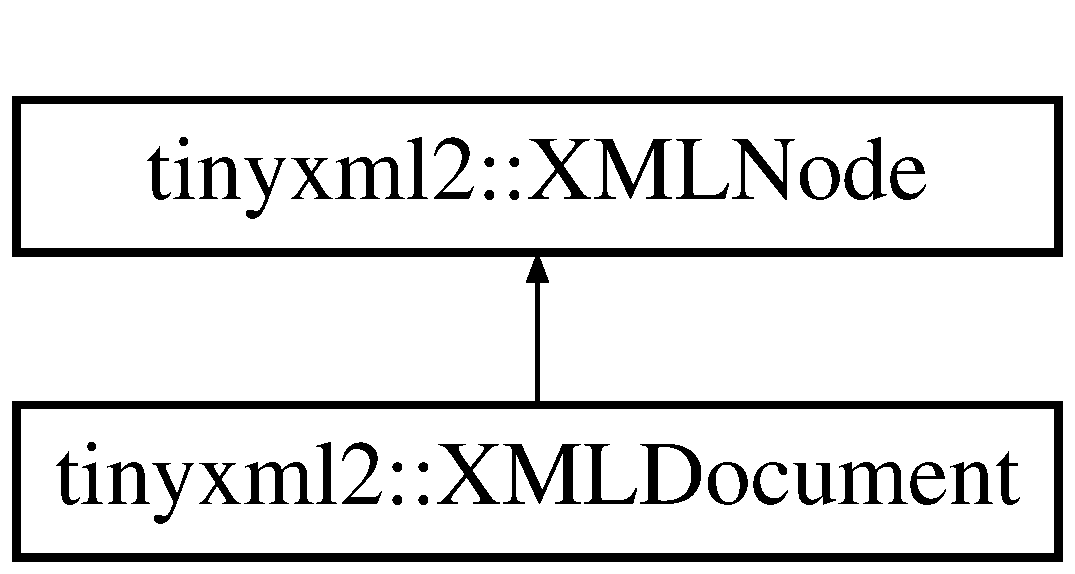
\includegraphics[height=2.000000cm]{classtinyxml2_1_1_x_m_l_document}
\end{center}
\end{figure}
\subsection*{Public Member Functions}
\begin{DoxyCompactItemize}
\item 
\hyperlink{classtinyxml2_1_1_x_m_l_document_af1574f76ebb619f25ef3f09eb2ba5188}{X\+M\+L\+Document} (bool process\+Entities=true, Whitespace=P\+R\+E\+S\+E\+R\+V\+E\+\_\+\+W\+H\+I\+T\+E\+S\+P\+A\+CE)\hypertarget{classtinyxml2_1_1_x_m_l_document_af1574f76ebb619f25ef3f09eb2ba5188}{}\label{classtinyxml2_1_1_x_m_l_document_af1574f76ebb619f25ef3f09eb2ba5188}

\begin{DoxyCompactList}\small\item\em constructor \end{DoxyCompactList}\item 
virtual \hyperlink{classtinyxml2_1_1_x_m_l_document}{X\+M\+L\+Document} $\ast$ \hyperlink{classtinyxml2_1_1_x_m_l_document_a3e185f880882bd978367bb55937735ec}{To\+Document} ()\hypertarget{classtinyxml2_1_1_x_m_l_document_a3e185f880882bd978367bb55937735ec}{}\label{classtinyxml2_1_1_x_m_l_document_a3e185f880882bd978367bb55937735ec}

\begin{DoxyCompactList}\small\item\em Safely cast to a Document, or null. \end{DoxyCompactList}\item 
virtual const \hyperlink{classtinyxml2_1_1_x_m_l_document}{X\+M\+L\+Document} $\ast$ {\bfseries To\+Document} () const \hypertarget{classtinyxml2_1_1_x_m_l_document_a15eb1a62afa18c66808031da647d1129}{}\label{classtinyxml2_1_1_x_m_l_document_a15eb1a62afa18c66808031da647d1129}

\item 
X\+M\+L\+Error \hyperlink{classtinyxml2_1_1_x_m_l_document_a1819bd34f540a7304c105a6232d25a1f}{Parse} (const char $\ast$xml, size\+\_\+t n\+Bytes=(size\+\_\+t)(-\/1))
\item 
X\+M\+L\+Error \hyperlink{classtinyxml2_1_1_x_m_l_document_a2ebd4647a8af5fc6831b294ac26a150a}{Load\+File} (const char $\ast$filename)
\item 
X\+M\+L\+Error \hyperlink{classtinyxml2_1_1_x_m_l_document_a5f1d330fad44c52f3d265338dd2a6dc2}{Load\+File} (F\+I\+LE $\ast$)
\item 
X\+M\+L\+Error \hyperlink{classtinyxml2_1_1_x_m_l_document_a73ac416b4a2aa0952e841220eb3da18f}{Save\+File} (const char $\ast$filename, bool compact=false)
\item 
X\+M\+L\+Error \hyperlink{classtinyxml2_1_1_x_m_l_document_a8b95779479a0035acc67b3a61dfe1b74}{Save\+File} (F\+I\+LE $\ast$fp, bool compact=false)
\item 
bool {\bfseries Process\+Entities} () const \hypertarget{classtinyxml2_1_1_x_m_l_document_adfcff7d0599cd520e9fcbb8891e1b678}{}\label{classtinyxml2_1_1_x_m_l_document_adfcff7d0599cd520e9fcbb8891e1b678}

\item 
Whitespace {\bfseries Whitespace\+Mode} () const \hypertarget{classtinyxml2_1_1_x_m_l_document_a94b3ea2f77c9ac831723984df5a02d01}{}\label{classtinyxml2_1_1_x_m_l_document_a94b3ea2f77c9ac831723984df5a02d01}

\item 
bool \hyperlink{classtinyxml2_1_1_x_m_l_document_a530649e9de7e5aa8df9c37f66197fcb6}{Has\+B\+OM} () const 
\item 
void \hyperlink{classtinyxml2_1_1_x_m_l_document_a14419b698f7c4b140df4e80f3f0c93b0}{Set\+B\+OM} (bool use\+B\+OM)
\item 
\hyperlink{classtinyxml2_1_1_x_m_l_element}{X\+M\+L\+Element} $\ast$ \hyperlink{classtinyxml2_1_1_x_m_l_document_ad2b70320d3c2a071c2f36928edff3e1c}{Root\+Element} ()
\item 
const \hyperlink{classtinyxml2_1_1_x_m_l_element}{X\+M\+L\+Element} $\ast$ {\bfseries Root\+Element} () const \hypertarget{classtinyxml2_1_1_x_m_l_document_a23a25b573d2adf3ee6075636c2a31c73}{}\label{classtinyxml2_1_1_x_m_l_document_a23a25b573d2adf3ee6075636c2a31c73}

\item 
void \hyperlink{classtinyxml2_1_1_x_m_l_document_a686ea28672c0e0c60383ec28148c1ac0}{Print} (\hyperlink{classtinyxml2_1_1_x_m_l_printer}{X\+M\+L\+Printer} $\ast$streamer=0) const 
\item 
virtual bool \hyperlink{classtinyxml2_1_1_x_m_l_document_aa08503d24898bf9992ae5e5fb8b0cf87}{Accept} (\hyperlink{classtinyxml2_1_1_x_m_l_visitor}{X\+M\+L\+Visitor} $\ast$visitor) const 
\item 
\hyperlink{classtinyxml2_1_1_x_m_l_element}{X\+M\+L\+Element} $\ast$ \hyperlink{classtinyxml2_1_1_x_m_l_document_a3c335a700a43d7c363a393142a23f234}{New\+Element} (const char $\ast$name)
\item 
\hyperlink{classtinyxml2_1_1_x_m_l_comment}{X\+M\+L\+Comment} $\ast$ \hyperlink{classtinyxml2_1_1_x_m_l_document_a386df0befd06aadb5e0cd21381aa955a}{New\+Comment} (const char $\ast$comment)
\item 
\hyperlink{classtinyxml2_1_1_x_m_l_text}{X\+M\+L\+Text} $\ast$ \hyperlink{classtinyxml2_1_1_x_m_l_document_acece5de77a0819f2341b08c1e1ed9987}{New\+Text} (const char $\ast$text)
\item 
\hyperlink{classtinyxml2_1_1_x_m_l_declaration}{X\+M\+L\+Declaration} $\ast$ \hyperlink{classtinyxml2_1_1_x_m_l_document_ae519030c0262fa2daff8993681990e16}{New\+Declaration} (const char $\ast$text=0)
\item 
\hyperlink{classtinyxml2_1_1_x_m_l_unknown}{X\+M\+L\+Unknown} $\ast$ \hyperlink{classtinyxml2_1_1_x_m_l_document_a4954f502c5fd7f49de54c3c0c99bb73d}{New\+Unknown} (const char $\ast$text)
\item 
void \hyperlink{classtinyxml2_1_1_x_m_l_document_ac1d6e2c7fcc1a660624ac4f68e96380d}{Delete\+Node} (\hyperlink{classtinyxml2_1_1_x_m_l_node}{X\+M\+L\+Node} $\ast$node)
\item 
void {\bfseries Set\+Error} (X\+M\+L\+Error error, const char $\ast$str1, const char $\ast$str2)\hypertarget{classtinyxml2_1_1_x_m_l_document_ae38d194e47336e4c96677ac77e2ac5d4}{}\label{classtinyxml2_1_1_x_m_l_document_ae38d194e47336e4c96677ac77e2ac5d4}

\item 
bool \hyperlink{classtinyxml2_1_1_x_m_l_document_abf0f9ac4c3aa5698a785937f71f7a69f}{Error} () const \hypertarget{classtinyxml2_1_1_x_m_l_document_abf0f9ac4c3aa5698a785937f71f7a69f}{}\label{classtinyxml2_1_1_x_m_l_document_abf0f9ac4c3aa5698a785937f71f7a69f}

\begin{DoxyCompactList}\small\item\em Return true if there was an error parsing the document. \end{DoxyCompactList}\item 
X\+M\+L\+Error \hyperlink{classtinyxml2_1_1_x_m_l_document_a34903418c9e83f27945c2c533839e350}{Error\+ID} () const \hypertarget{classtinyxml2_1_1_x_m_l_document_a34903418c9e83f27945c2c533839e350}{}\label{classtinyxml2_1_1_x_m_l_document_a34903418c9e83f27945c2c533839e350}

\begin{DoxyCompactList}\small\item\em Return the error\+ID. \end{DoxyCompactList}\item 
const char $\ast$ {\bfseries Error\+Name} () const \hypertarget{classtinyxml2_1_1_x_m_l_document_a7ff8b68f87042d535841b0afd2c82161}{}\label{classtinyxml2_1_1_x_m_l_document_a7ff8b68f87042d535841b0afd2c82161}

\item 
const char $\ast$ \hyperlink{classtinyxml2_1_1_x_m_l_document_a016ccebecee36fe92084b5dfee6cc072}{Get\+Error\+Str1} () const \hypertarget{classtinyxml2_1_1_x_m_l_document_a016ccebecee36fe92084b5dfee6cc072}{}\label{classtinyxml2_1_1_x_m_l_document_a016ccebecee36fe92084b5dfee6cc072}

\begin{DoxyCompactList}\small\item\em Return a possibly helpful diagnostic location or string. \end{DoxyCompactList}\item 
const char $\ast$ \hyperlink{classtinyxml2_1_1_x_m_l_document_a88f6b44bd019033bda28abd31fe257b2}{Get\+Error\+Str2} () const \hypertarget{classtinyxml2_1_1_x_m_l_document_a88f6b44bd019033bda28abd31fe257b2}{}\label{classtinyxml2_1_1_x_m_l_document_a88f6b44bd019033bda28abd31fe257b2}

\begin{DoxyCompactList}\small\item\em Return a possibly helpful secondary diagnostic location or string. \end{DoxyCompactList}\item 
void \hyperlink{classtinyxml2_1_1_x_m_l_document_a7545cc9a9a67eee9307c001aa316a388}{Print\+Error} () const \hypertarget{classtinyxml2_1_1_x_m_l_document_a7545cc9a9a67eee9307c001aa316a388}{}\label{classtinyxml2_1_1_x_m_l_document_a7545cc9a9a67eee9307c001aa316a388}

\begin{DoxyCompactList}\small\item\em If there is an error, print it to stdout. \end{DoxyCompactList}\item 
void \hyperlink{classtinyxml2_1_1_x_m_l_document_a65656b0b2cbc822708eb351504178aaf}{Clear} ()\hypertarget{classtinyxml2_1_1_x_m_l_document_a65656b0b2cbc822708eb351504178aaf}{}\label{classtinyxml2_1_1_x_m_l_document_a65656b0b2cbc822708eb351504178aaf}

\begin{DoxyCompactList}\small\item\em Clear the document, resetting it to the initial state. \end{DoxyCompactList}\item 
char $\ast$ {\bfseries Identify} (char $\ast$p, \hyperlink{classtinyxml2_1_1_x_m_l_node}{X\+M\+L\+Node} $\ast$$\ast$node)\hypertarget{classtinyxml2_1_1_x_m_l_document_a25827d1bec509ad566a107e5853ed040}{}\label{classtinyxml2_1_1_x_m_l_document_a25827d1bec509ad566a107e5853ed040}

\item 
virtual \hyperlink{classtinyxml2_1_1_x_m_l_node}{X\+M\+L\+Node} $\ast$ \hyperlink{classtinyxml2_1_1_x_m_l_document_a57c8511ed9f83aa3e20909a3db3f83d0}{Shallow\+Clone} (\hyperlink{classtinyxml2_1_1_x_m_l_document}{X\+M\+L\+Document} $\ast$) const 
\item 
virtual bool \hyperlink{classtinyxml2_1_1_x_m_l_document_a12eac66c6e45d074d5cc47319868cd66}{Shallow\+Equal} (const \hyperlink{classtinyxml2_1_1_x_m_l_node}{X\+M\+L\+Node} $\ast$) const 
\end{DoxyCompactItemize}
\subsection*{Friends}
\begin{DoxyCompactItemize}
\item 
class {\bfseries X\+M\+L\+Element}\hypertarget{classtinyxml2_1_1_x_m_l_document_ac2fba9b6e452829dd892f7392c24e0eb}{}\label{classtinyxml2_1_1_x_m_l_document_ac2fba9b6e452829dd892f7392c24e0eb}

\end{DoxyCompactItemize}
\subsection*{Additional Inherited Members}


\subsection{Detailed Description}
A Document binds together all the functionality. It can be saved, loaded, and printed to the screen. All Nodes are connected and allocated to a Document. If the Document is deleted, all its Nodes are also deleted. 

\subsection{Member Function Documentation}
\index{tinyxml2\+::\+X\+M\+L\+Document@{tinyxml2\+::\+X\+M\+L\+Document}!Accept@{Accept}}
\index{Accept@{Accept}!tinyxml2\+::\+X\+M\+L\+Document@{tinyxml2\+::\+X\+M\+L\+Document}}
\subsubsection[{\texorpdfstring{Accept(\+X\+M\+L\+Visitor $\ast$visitor) const }{Accept(XMLVisitor *visitor) const }}]{\setlength{\rightskip}{0pt plus 5cm}bool tinyxml2\+::\+X\+M\+L\+Document\+::\+Accept (
\begin{DoxyParamCaption}
\item[{{\bf X\+M\+L\+Visitor} $\ast$}]{visitor}
\end{DoxyParamCaption}
) const\hspace{0.3cm}{\ttfamily [virtual]}}\hypertarget{classtinyxml2_1_1_x_m_l_document_aa08503d24898bf9992ae5e5fb8b0cf87}{}\label{classtinyxml2_1_1_x_m_l_document_aa08503d24898bf9992ae5e5fb8b0cf87}
Accept a hierarchical visit of the nodes in the Tiny\+X\+M\+L-\/2 D\+OM. Every node in the X\+ML tree will be conditionally visited and the host will be called back via the \hyperlink{classtinyxml2_1_1_x_m_l_visitor}{X\+M\+L\+Visitor} interface.

This is essentially a S\+AX interface for Tiny\+X\+M\+L-\/2. (Note however it doesn\textquotesingle{}t re-\/parse the X\+ML for the callbacks, so the performance of Tiny\+X\+M\+L-\/2 is unchanged by using this interface versus any other.)

The interface has been based on ideas from\+:


\begin{DoxyItemize}
\item \href{http://www.saxproject.org/}{\tt http\+://www.\+saxproject.\+org/}
\item \href{http://c2.com/cgi/wiki?HierarchicalVisitorPattern}{\tt http\+://c2.\+com/cgi/wiki?\+Hierarchical\+Visitor\+Pattern}
\end{DoxyItemize}

Which are both good references for \char`\"{}visiting\char`\"{}.

An example of using \hyperlink{classtinyxml2_1_1_x_m_l_document_aa08503d24898bf9992ae5e5fb8b0cf87}{Accept()}\+: \begin{DoxyVerb}XMLPrinter printer;
tinyxmlDoc.Accept( &printer );
const char* xmlcstr = printer.CStr();
\end{DoxyVerb}
 

Implements \hyperlink{classtinyxml2_1_1_x_m_l_node_a366ad0e9b9ae8d1b18c00f903994b7a9}{tinyxml2\+::\+X\+M\+L\+Node}.

\index{tinyxml2\+::\+X\+M\+L\+Document@{tinyxml2\+::\+X\+M\+L\+Document}!Delete\+Node@{Delete\+Node}}
\index{Delete\+Node@{Delete\+Node}!tinyxml2\+::\+X\+M\+L\+Document@{tinyxml2\+::\+X\+M\+L\+Document}}
\subsubsection[{\texorpdfstring{Delete\+Node(\+X\+M\+L\+Node $\ast$node)}{DeleteNode(XMLNode *node)}}]{\setlength{\rightskip}{0pt plus 5cm}void tinyxml2\+::\+X\+M\+L\+Document\+::\+Delete\+Node (
\begin{DoxyParamCaption}
\item[{{\bf X\+M\+L\+Node} $\ast$}]{node}
\end{DoxyParamCaption}
)}\hypertarget{classtinyxml2_1_1_x_m_l_document_ac1d6e2c7fcc1a660624ac4f68e96380d}{}\label{classtinyxml2_1_1_x_m_l_document_ac1d6e2c7fcc1a660624ac4f68e96380d}
Delete a node associated with this document. It will be unlinked from the D\+OM. \index{tinyxml2\+::\+X\+M\+L\+Document@{tinyxml2\+::\+X\+M\+L\+Document}!Has\+B\+OM@{Has\+B\+OM}}
\index{Has\+B\+OM@{Has\+B\+OM}!tinyxml2\+::\+X\+M\+L\+Document@{tinyxml2\+::\+X\+M\+L\+Document}}
\subsubsection[{\texorpdfstring{Has\+B\+O\+M() const }{HasBOM() const }}]{\setlength{\rightskip}{0pt plus 5cm}bool tinyxml2\+::\+X\+M\+L\+Document\+::\+Has\+B\+OM (
\begin{DoxyParamCaption}
{}
\end{DoxyParamCaption}
) const\hspace{0.3cm}{\ttfamily [inline]}}\hypertarget{classtinyxml2_1_1_x_m_l_document_a530649e9de7e5aa8df9c37f66197fcb6}{}\label{classtinyxml2_1_1_x_m_l_document_a530649e9de7e5aa8df9c37f66197fcb6}
Returns true if this document has a leading Byte Order Mark of U\+T\+F8. \index{tinyxml2\+::\+X\+M\+L\+Document@{tinyxml2\+::\+X\+M\+L\+Document}!Load\+File@{Load\+File}}
\index{Load\+File@{Load\+File}!tinyxml2\+::\+X\+M\+L\+Document@{tinyxml2\+::\+X\+M\+L\+Document}}
\subsubsection[{\texorpdfstring{Load\+File(const char $\ast$filename)}{LoadFile(const char *filename)}}]{\setlength{\rightskip}{0pt plus 5cm}X\+M\+L\+Error tinyxml2\+::\+X\+M\+L\+Document\+::\+Load\+File (
\begin{DoxyParamCaption}
\item[{const char $\ast$}]{filename}
\end{DoxyParamCaption}
)}\hypertarget{classtinyxml2_1_1_x_m_l_document_a2ebd4647a8af5fc6831b294ac26a150a}{}\label{classtinyxml2_1_1_x_m_l_document_a2ebd4647a8af5fc6831b294ac26a150a}
Load an X\+ML file from disk. Returns X\+M\+L\+\_\+\+N\+O\+\_\+\+E\+R\+R\+OR (0) on success, or an error\+ID. \index{tinyxml2\+::\+X\+M\+L\+Document@{tinyxml2\+::\+X\+M\+L\+Document}!Load\+File@{Load\+File}}
\index{Load\+File@{Load\+File}!tinyxml2\+::\+X\+M\+L\+Document@{tinyxml2\+::\+X\+M\+L\+Document}}
\subsubsection[{\texorpdfstring{Load\+File(\+F\+I\+L\+E $\ast$)}{LoadFile(FILE *)}}]{\setlength{\rightskip}{0pt plus 5cm}X\+M\+L\+Error tinyxml2\+::\+X\+M\+L\+Document\+::\+Load\+File (
\begin{DoxyParamCaption}
\item[{F\+I\+LE $\ast$}]{fp}
\end{DoxyParamCaption}
)}\hypertarget{classtinyxml2_1_1_x_m_l_document_a5f1d330fad44c52f3d265338dd2a6dc2}{}\label{classtinyxml2_1_1_x_m_l_document_a5f1d330fad44c52f3d265338dd2a6dc2}
Load an X\+ML file from disk. You are responsible for providing and closing the F\+I\+L\+E$\ast$.

N\+O\+TE\+: The file should be opened as binary (\char`\"{}rb\char`\"{}) not text in order for Tiny\+X\+M\+L-\/2 to correctly do newline normalization.

Returns X\+M\+L\+\_\+\+N\+O\+\_\+\+E\+R\+R\+OR (0) on success, or an error\+ID. \index{tinyxml2\+::\+X\+M\+L\+Document@{tinyxml2\+::\+X\+M\+L\+Document}!New\+Comment@{New\+Comment}}
\index{New\+Comment@{New\+Comment}!tinyxml2\+::\+X\+M\+L\+Document@{tinyxml2\+::\+X\+M\+L\+Document}}
\subsubsection[{\texorpdfstring{New\+Comment(const char $\ast$comment)}{NewComment(const char *comment)}}]{\setlength{\rightskip}{0pt plus 5cm}{\bf X\+M\+L\+Comment} $\ast$ tinyxml2\+::\+X\+M\+L\+Document\+::\+New\+Comment (
\begin{DoxyParamCaption}
\item[{const char $\ast$}]{comment}
\end{DoxyParamCaption}
)}\hypertarget{classtinyxml2_1_1_x_m_l_document_a386df0befd06aadb5e0cd21381aa955a}{}\label{classtinyxml2_1_1_x_m_l_document_a386df0befd06aadb5e0cd21381aa955a}
Create a new Comment associated with this Document. The memory for the Comment is managed by the Document. \index{tinyxml2\+::\+X\+M\+L\+Document@{tinyxml2\+::\+X\+M\+L\+Document}!New\+Declaration@{New\+Declaration}}
\index{New\+Declaration@{New\+Declaration}!tinyxml2\+::\+X\+M\+L\+Document@{tinyxml2\+::\+X\+M\+L\+Document}}
\subsubsection[{\texorpdfstring{New\+Declaration(const char $\ast$text=0)}{NewDeclaration(const char *text=0)}}]{\setlength{\rightskip}{0pt plus 5cm}{\bf X\+M\+L\+Declaration} $\ast$ tinyxml2\+::\+X\+M\+L\+Document\+::\+New\+Declaration (
\begin{DoxyParamCaption}
\item[{const char $\ast$}]{text = {\ttfamily 0}}
\end{DoxyParamCaption}
)}\hypertarget{classtinyxml2_1_1_x_m_l_document_ae519030c0262fa2daff8993681990e16}{}\label{classtinyxml2_1_1_x_m_l_document_ae519030c0262fa2daff8993681990e16}
Create a new Declaration associated with this Document. The memory for the object is managed by the Document.

If the \textquotesingle{}text\textquotesingle{} param is null, the standard declaration is used.\+: \begin{DoxyVerb}    <?xml version="1.0" encoding="UTF-8"?>
\end{DoxyVerb}
 \index{tinyxml2\+::\+X\+M\+L\+Document@{tinyxml2\+::\+X\+M\+L\+Document}!New\+Element@{New\+Element}}
\index{New\+Element@{New\+Element}!tinyxml2\+::\+X\+M\+L\+Document@{tinyxml2\+::\+X\+M\+L\+Document}}
\subsubsection[{\texorpdfstring{New\+Element(const char $\ast$name)}{NewElement(const char *name)}}]{\setlength{\rightskip}{0pt plus 5cm}{\bf X\+M\+L\+Element} $\ast$ tinyxml2\+::\+X\+M\+L\+Document\+::\+New\+Element (
\begin{DoxyParamCaption}
\item[{const char $\ast$}]{name}
\end{DoxyParamCaption}
)}\hypertarget{classtinyxml2_1_1_x_m_l_document_a3c335a700a43d7c363a393142a23f234}{}\label{classtinyxml2_1_1_x_m_l_document_a3c335a700a43d7c363a393142a23f234}
Create a new Element associated with this Document. The memory for the Element is managed by the Document. \index{tinyxml2\+::\+X\+M\+L\+Document@{tinyxml2\+::\+X\+M\+L\+Document}!New\+Text@{New\+Text}}
\index{New\+Text@{New\+Text}!tinyxml2\+::\+X\+M\+L\+Document@{tinyxml2\+::\+X\+M\+L\+Document}}
\subsubsection[{\texorpdfstring{New\+Text(const char $\ast$text)}{NewText(const char *text)}}]{\setlength{\rightskip}{0pt plus 5cm}{\bf X\+M\+L\+Text} $\ast$ tinyxml2\+::\+X\+M\+L\+Document\+::\+New\+Text (
\begin{DoxyParamCaption}
\item[{const char $\ast$}]{text}
\end{DoxyParamCaption}
)}\hypertarget{classtinyxml2_1_1_x_m_l_document_acece5de77a0819f2341b08c1e1ed9987}{}\label{classtinyxml2_1_1_x_m_l_document_acece5de77a0819f2341b08c1e1ed9987}
Create a new Text associated with this Document. The memory for the Text is managed by the Document. \index{tinyxml2\+::\+X\+M\+L\+Document@{tinyxml2\+::\+X\+M\+L\+Document}!New\+Unknown@{New\+Unknown}}
\index{New\+Unknown@{New\+Unknown}!tinyxml2\+::\+X\+M\+L\+Document@{tinyxml2\+::\+X\+M\+L\+Document}}
\subsubsection[{\texorpdfstring{New\+Unknown(const char $\ast$text)}{NewUnknown(const char *text)}}]{\setlength{\rightskip}{0pt plus 5cm}{\bf X\+M\+L\+Unknown} $\ast$ tinyxml2\+::\+X\+M\+L\+Document\+::\+New\+Unknown (
\begin{DoxyParamCaption}
\item[{const char $\ast$}]{text}
\end{DoxyParamCaption}
)}\hypertarget{classtinyxml2_1_1_x_m_l_document_a4954f502c5fd7f49de54c3c0c99bb73d}{}\label{classtinyxml2_1_1_x_m_l_document_a4954f502c5fd7f49de54c3c0c99bb73d}
Create a new Unknown associated with this Document. The memory for the object is managed by the Document. \index{tinyxml2\+::\+X\+M\+L\+Document@{tinyxml2\+::\+X\+M\+L\+Document}!Parse@{Parse}}
\index{Parse@{Parse}!tinyxml2\+::\+X\+M\+L\+Document@{tinyxml2\+::\+X\+M\+L\+Document}}
\subsubsection[{\texorpdfstring{Parse(const char $\ast$xml, size\+\_\+t n\+Bytes=(size\+\_\+t)(-\/1))}{Parse(const char *xml, size_t nBytes=(size_t)(-1))}}]{\setlength{\rightskip}{0pt plus 5cm}X\+M\+L\+Error tinyxml2\+::\+X\+M\+L\+Document\+::\+Parse (
\begin{DoxyParamCaption}
\item[{const char $\ast$}]{xml, }
\item[{size\+\_\+t}]{n\+Bytes = {\ttfamily (size\+\_\+t)(-\/1)}}
\end{DoxyParamCaption}
)}\hypertarget{classtinyxml2_1_1_x_m_l_document_a1819bd34f540a7304c105a6232d25a1f}{}\label{classtinyxml2_1_1_x_m_l_document_a1819bd34f540a7304c105a6232d25a1f}
Parse an X\+ML file from a character string. Returns X\+M\+L\+\_\+\+N\+O\+\_\+\+E\+R\+R\+OR (0) on success, or an error\+ID.

You may optionally pass in the \textquotesingle{}n\+Bytes\textquotesingle{}, which is the number of bytes which will be parsed. If not specified, Tiny\+X\+M\+L-\/2 will assume \textquotesingle{}xml\textquotesingle{} points to a null terminated string. \index{tinyxml2\+::\+X\+M\+L\+Document@{tinyxml2\+::\+X\+M\+L\+Document}!Print@{Print}}
\index{Print@{Print}!tinyxml2\+::\+X\+M\+L\+Document@{tinyxml2\+::\+X\+M\+L\+Document}}
\subsubsection[{\texorpdfstring{Print(\+X\+M\+L\+Printer $\ast$streamer=0) const }{Print(XMLPrinter *streamer=0) const }}]{\setlength{\rightskip}{0pt plus 5cm}void tinyxml2\+::\+X\+M\+L\+Document\+::\+Print (
\begin{DoxyParamCaption}
\item[{{\bf X\+M\+L\+Printer} $\ast$}]{streamer = {\ttfamily 0}}
\end{DoxyParamCaption}
) const}\hypertarget{classtinyxml2_1_1_x_m_l_document_a686ea28672c0e0c60383ec28148c1ac0}{}\label{classtinyxml2_1_1_x_m_l_document_a686ea28672c0e0c60383ec28148c1ac0}
Print the Document. If the Printer is not provided, it will print to stdout. If you provide Printer, this can print to a file\+: \begin{DoxyVerb}XMLPrinter printer( fp );
doc.Print( &printer );
\end{DoxyVerb}


Or you can use a printer to print to memory\+: \begin{DoxyVerb}XMLPrinter printer;
doc.Print( &printer );
// printer.CStr() has a const char* to the XML
\end{DoxyVerb}
 \index{tinyxml2\+::\+X\+M\+L\+Document@{tinyxml2\+::\+X\+M\+L\+Document}!Root\+Element@{Root\+Element}}
\index{Root\+Element@{Root\+Element}!tinyxml2\+::\+X\+M\+L\+Document@{tinyxml2\+::\+X\+M\+L\+Document}}
\subsubsection[{\texorpdfstring{Root\+Element()}{RootElement()}}]{\setlength{\rightskip}{0pt plus 5cm}{\bf X\+M\+L\+Element}$\ast$ tinyxml2\+::\+X\+M\+L\+Document\+::\+Root\+Element (
\begin{DoxyParamCaption}
{}
\end{DoxyParamCaption}
)\hspace{0.3cm}{\ttfamily [inline]}}\hypertarget{classtinyxml2_1_1_x_m_l_document_ad2b70320d3c2a071c2f36928edff3e1c}{}\label{classtinyxml2_1_1_x_m_l_document_ad2b70320d3c2a071c2f36928edff3e1c}
Return the root element of D\+OM. Equivalent to \hyperlink{classtinyxml2_1_1_x_m_l_node_a4a38e0da23f4d97673a86c77d5cae5c2}{First\+Child\+Element()}. To get the first node, use First\+Child(). \index{tinyxml2\+::\+X\+M\+L\+Document@{tinyxml2\+::\+X\+M\+L\+Document}!Save\+File@{Save\+File}}
\index{Save\+File@{Save\+File}!tinyxml2\+::\+X\+M\+L\+Document@{tinyxml2\+::\+X\+M\+L\+Document}}
\subsubsection[{\texorpdfstring{Save\+File(const char $\ast$filename, bool compact=false)}{SaveFile(const char *filename, bool compact=false)}}]{\setlength{\rightskip}{0pt plus 5cm}X\+M\+L\+Error tinyxml2\+::\+X\+M\+L\+Document\+::\+Save\+File (
\begin{DoxyParamCaption}
\item[{const char $\ast$}]{filename, }
\item[{bool}]{compact = {\ttfamily false}}
\end{DoxyParamCaption}
)}\hypertarget{classtinyxml2_1_1_x_m_l_document_a73ac416b4a2aa0952e841220eb3da18f}{}\label{classtinyxml2_1_1_x_m_l_document_a73ac416b4a2aa0952e841220eb3da18f}
Save the X\+ML file to disk. Returns X\+M\+L\+\_\+\+N\+O\+\_\+\+E\+R\+R\+OR (0) on success, or an error\+ID. \index{tinyxml2\+::\+X\+M\+L\+Document@{tinyxml2\+::\+X\+M\+L\+Document}!Save\+File@{Save\+File}}
\index{Save\+File@{Save\+File}!tinyxml2\+::\+X\+M\+L\+Document@{tinyxml2\+::\+X\+M\+L\+Document}}
\subsubsection[{\texorpdfstring{Save\+File(\+F\+I\+L\+E $\ast$fp, bool compact=false)}{SaveFile(FILE *fp, bool compact=false)}}]{\setlength{\rightskip}{0pt plus 5cm}X\+M\+L\+Error tinyxml2\+::\+X\+M\+L\+Document\+::\+Save\+File (
\begin{DoxyParamCaption}
\item[{F\+I\+LE $\ast$}]{fp, }
\item[{bool}]{compact = {\ttfamily false}}
\end{DoxyParamCaption}
)}\hypertarget{classtinyxml2_1_1_x_m_l_document_a8b95779479a0035acc67b3a61dfe1b74}{}\label{classtinyxml2_1_1_x_m_l_document_a8b95779479a0035acc67b3a61dfe1b74}
Save the X\+ML file to disk. You are responsible for providing and closing the F\+I\+L\+E$\ast$.

Returns X\+M\+L\+\_\+\+N\+O\+\_\+\+E\+R\+R\+OR (0) on success, or an error\+ID. \index{tinyxml2\+::\+X\+M\+L\+Document@{tinyxml2\+::\+X\+M\+L\+Document}!Set\+B\+OM@{Set\+B\+OM}}
\index{Set\+B\+OM@{Set\+B\+OM}!tinyxml2\+::\+X\+M\+L\+Document@{tinyxml2\+::\+X\+M\+L\+Document}}
\subsubsection[{\texorpdfstring{Set\+B\+O\+M(bool use\+B\+O\+M)}{SetBOM(bool useBOM)}}]{\setlength{\rightskip}{0pt plus 5cm}void tinyxml2\+::\+X\+M\+L\+Document\+::\+Set\+B\+OM (
\begin{DoxyParamCaption}
\item[{bool}]{use\+B\+OM}
\end{DoxyParamCaption}
)\hspace{0.3cm}{\ttfamily [inline]}}\hypertarget{classtinyxml2_1_1_x_m_l_document_a14419b698f7c4b140df4e80f3f0c93b0}{}\label{classtinyxml2_1_1_x_m_l_document_a14419b698f7c4b140df4e80f3f0c93b0}
Sets whether to write the B\+OM when writing the file. \index{tinyxml2\+::\+X\+M\+L\+Document@{tinyxml2\+::\+X\+M\+L\+Document}!Shallow\+Clone@{Shallow\+Clone}}
\index{Shallow\+Clone@{Shallow\+Clone}!tinyxml2\+::\+X\+M\+L\+Document@{tinyxml2\+::\+X\+M\+L\+Document}}
\subsubsection[{\texorpdfstring{Shallow\+Clone(\+X\+M\+L\+Document $\ast$) const }{ShallowClone(XMLDocument *) const }}]{\setlength{\rightskip}{0pt plus 5cm}virtual {\bf X\+M\+L\+Node}$\ast$ tinyxml2\+::\+X\+M\+L\+Document\+::\+Shallow\+Clone (
\begin{DoxyParamCaption}
\item[{{\bf X\+M\+L\+Document} $\ast$}]{document}
\end{DoxyParamCaption}
) const\hspace{0.3cm}{\ttfamily [inline]}, {\ttfamily [virtual]}}\hypertarget{classtinyxml2_1_1_x_m_l_document_a57c8511ed9f83aa3e20909a3db3f83d0}{}\label{classtinyxml2_1_1_x_m_l_document_a57c8511ed9f83aa3e20909a3db3f83d0}
Make a copy of this node, but not its children. You may pass in a Document pointer that will be the owner of the new Node. If the \textquotesingle{}document\textquotesingle{} is null, then the node returned will be allocated from the current Document. (this-\/$>$\hyperlink{classtinyxml2_1_1_x_m_l_node_af343d1ef0b45c0020e62d784d7e67a68}{Get\+Document()})

Note\+: if called on a \hyperlink{classtinyxml2_1_1_x_m_l_document}{X\+M\+L\+Document}, this will return null. 

Implements \hyperlink{classtinyxml2_1_1_x_m_l_node_a83e3524e2ecea25eeab630c7ab113627}{tinyxml2\+::\+X\+M\+L\+Node}.

\index{tinyxml2\+::\+X\+M\+L\+Document@{tinyxml2\+::\+X\+M\+L\+Document}!Shallow\+Equal@{Shallow\+Equal}}
\index{Shallow\+Equal@{Shallow\+Equal}!tinyxml2\+::\+X\+M\+L\+Document@{tinyxml2\+::\+X\+M\+L\+Document}}
\subsubsection[{\texorpdfstring{Shallow\+Equal(const X\+M\+L\+Node $\ast$) const }{ShallowEqual(const XMLNode *) const }}]{\setlength{\rightskip}{0pt plus 5cm}virtual bool tinyxml2\+::\+X\+M\+L\+Document\+::\+Shallow\+Equal (
\begin{DoxyParamCaption}
\item[{const {\bf X\+M\+L\+Node} $\ast$}]{compare}
\end{DoxyParamCaption}
) const\hspace{0.3cm}{\ttfamily [inline]}, {\ttfamily [virtual]}}\hypertarget{classtinyxml2_1_1_x_m_l_document_a12eac66c6e45d074d5cc47319868cd66}{}\label{classtinyxml2_1_1_x_m_l_document_a12eac66c6e45d074d5cc47319868cd66}
Test if 2 nodes are the same, but don\textquotesingle{}t test children. The 2 nodes do not need to be in the same Document.

Note\+: if called on a \hyperlink{classtinyxml2_1_1_x_m_l_document}{X\+M\+L\+Document}, this will return false. 

Implements \hyperlink{classtinyxml2_1_1_x_m_l_node_ac50408e91e095237f45716092ac2bddc}{tinyxml2\+::\+X\+M\+L\+Node}.



The documentation for this class was generated from the following files\+:\begin{DoxyCompactItemize}
\item 
src/tinyxml2.\+h\item 
src/tinyxml2.\+cpp\end{DoxyCompactItemize}

\hypertarget{classtinyxml2_1_1_x_m_l_element}{}\section{tinyxml2\+:\+:X\+M\+L\+Element Class Reference}
\label{classtinyxml2_1_1_x_m_l_element}\index{tinyxml2\+::\+X\+M\+L\+Element@{tinyxml2\+::\+X\+M\+L\+Element}}


{\ttfamily \#include $<$tinyxml2.\+h$>$}

Inheritance diagram for tinyxml2\+:\+:X\+M\+L\+Element\+:\begin{figure}[H]
\begin{center}
\leavevmode
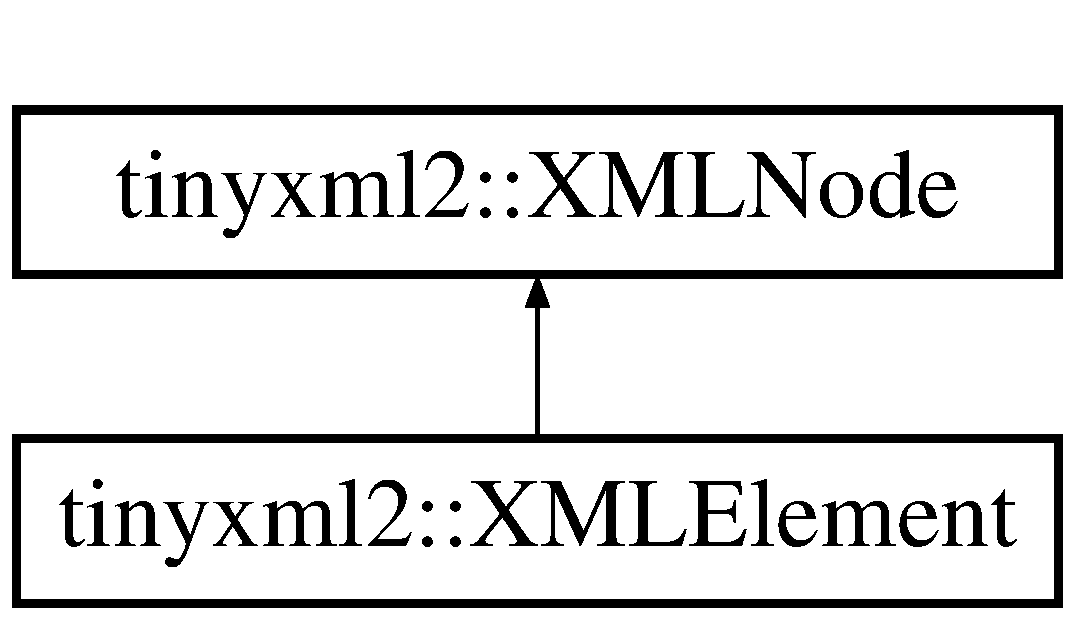
\includegraphics[height=2.000000cm]{classtinyxml2_1_1_x_m_l_element}
\end{center}
\end{figure}
\subsection*{Public Types}
\begin{DoxyCompactItemize}
\item 
enum \{ {\bfseries O\+P\+EN}, 
{\bfseries C\+L\+O\+S\+ED}, 
{\bfseries C\+L\+O\+S\+I\+NG}
 \}\hypertarget{classtinyxml2_1_1_x_m_l_element_a07a6ce25c17aaa505933db57f2373e50}{}\label{classtinyxml2_1_1_x_m_l_element_a07a6ce25c17aaa505933db57f2373e50}

\end{DoxyCompactItemize}
\subsection*{Public Member Functions}
\begin{DoxyCompactItemize}
\item 
const char $\ast$ \hyperlink{classtinyxml2_1_1_x_m_l_element_a8bff355472bce2c60d4b50a212bf7f5f}{Name} () const \hypertarget{classtinyxml2_1_1_x_m_l_element_a8bff355472bce2c60d4b50a212bf7f5f}{}\label{classtinyxml2_1_1_x_m_l_element_a8bff355472bce2c60d4b50a212bf7f5f}

\begin{DoxyCompactList}\small\item\em Get the name of an element (which is the \hyperlink{classtinyxml2_1_1_x_m_l_node_a92835c779871918f9af569bfe9669fe6}{Value()} of the node.) \end{DoxyCompactList}\item 
void \hyperlink{classtinyxml2_1_1_x_m_l_element_a97712009a530d8cb8a63bf705f02b4f1}{Set\+Name} (const char $\ast$str, bool static\+Mem=false)\hypertarget{classtinyxml2_1_1_x_m_l_element_a97712009a530d8cb8a63bf705f02b4f1}{}\label{classtinyxml2_1_1_x_m_l_element_a97712009a530d8cb8a63bf705f02b4f1}

\begin{DoxyCompactList}\small\item\em Set the name of the element. \end{DoxyCompactList}\item 
virtual \hyperlink{classtinyxml2_1_1_x_m_l_element}{X\+M\+L\+Element} $\ast$ \hyperlink{classtinyxml2_1_1_x_m_l_element_ad9ff5c2dbc15df36cf664ce1b0ea0a5d}{To\+Element} ()\hypertarget{classtinyxml2_1_1_x_m_l_element_ad9ff5c2dbc15df36cf664ce1b0ea0a5d}{}\label{classtinyxml2_1_1_x_m_l_element_ad9ff5c2dbc15df36cf664ce1b0ea0a5d}

\begin{DoxyCompactList}\small\item\em Safely cast to an Element, or null. \end{DoxyCompactList}\item 
virtual const \hyperlink{classtinyxml2_1_1_x_m_l_element}{X\+M\+L\+Element} $\ast$ {\bfseries To\+Element} () const \hypertarget{classtinyxml2_1_1_x_m_l_element_a55acab615353ddabab48271f95816b0d}{}\label{classtinyxml2_1_1_x_m_l_element_a55acab615353ddabab48271f95816b0d}

\item 
virtual bool \hyperlink{classtinyxml2_1_1_x_m_l_element_a36d65438991a1e85096caf39ad13a099}{Accept} (\hyperlink{classtinyxml2_1_1_x_m_l_visitor}{X\+M\+L\+Visitor} $\ast$visitor) const 
\item 
const char $\ast$ \hyperlink{classtinyxml2_1_1_x_m_l_element_a7bdebdf1888074087237f3dd03912740}{Attribute} (const char $\ast$name, const char $\ast$value=0) const 
\item 
int \hyperlink{classtinyxml2_1_1_x_m_l_element_af86f05771c11a73a2896b662bb589ef5}{Int\+Attribute} (const char $\ast$name) const 
\item 
unsigned \hyperlink{classtinyxml2_1_1_x_m_l_element_aa5a41367b5118acec42a87f5f94cec2d}{Unsigned\+Attribute} (const char $\ast$name) const \hypertarget{classtinyxml2_1_1_x_m_l_element_aa5a41367b5118acec42a87f5f94cec2d}{}\label{classtinyxml2_1_1_x_m_l_element_aa5a41367b5118acec42a87f5f94cec2d}

\begin{DoxyCompactList}\small\item\em See \hyperlink{classtinyxml2_1_1_x_m_l_element_af86f05771c11a73a2896b662bb589ef5}{Int\+Attribute()} \end{DoxyCompactList}\item 
bool \hyperlink{classtinyxml2_1_1_x_m_l_element_a34811e4d1881e4ecc95c49f0f3799115}{Bool\+Attribute} (const char $\ast$name) const \hypertarget{classtinyxml2_1_1_x_m_l_element_a34811e4d1881e4ecc95c49f0f3799115}{}\label{classtinyxml2_1_1_x_m_l_element_a34811e4d1881e4ecc95c49f0f3799115}

\begin{DoxyCompactList}\small\item\em See \hyperlink{classtinyxml2_1_1_x_m_l_element_af86f05771c11a73a2896b662bb589ef5}{Int\+Attribute()} \end{DoxyCompactList}\item 
double \hyperlink{classtinyxml2_1_1_x_m_l_element_a536922a5cae9c9769a3dc1b7a8ff0d44}{Double\+Attribute} (const char $\ast$name) const \hypertarget{classtinyxml2_1_1_x_m_l_element_a536922a5cae9c9769a3dc1b7a8ff0d44}{}\label{classtinyxml2_1_1_x_m_l_element_a536922a5cae9c9769a3dc1b7a8ff0d44}

\begin{DoxyCompactList}\small\item\em See \hyperlink{classtinyxml2_1_1_x_m_l_element_af86f05771c11a73a2896b662bb589ef5}{Int\+Attribute()} \end{DoxyCompactList}\item 
float \hyperlink{classtinyxml2_1_1_x_m_l_element_a33b69f123f995aff966d2e351bc51b1f}{Float\+Attribute} (const char $\ast$name) const \hypertarget{classtinyxml2_1_1_x_m_l_element_a33b69f123f995aff966d2e351bc51b1f}{}\label{classtinyxml2_1_1_x_m_l_element_a33b69f123f995aff966d2e351bc51b1f}

\begin{DoxyCompactList}\small\item\em See \hyperlink{classtinyxml2_1_1_x_m_l_element_af86f05771c11a73a2896b662bb589ef5}{Int\+Attribute()} \end{DoxyCompactList}\item 
X\+M\+L\+Error \hyperlink{classtinyxml2_1_1_x_m_l_element_a8b92c729346aa8ea9acd59ed3e9f2378}{Query\+Int\+Attribute} (const char $\ast$name, int $\ast$value) const 
\item 
X\+M\+L\+Error \hyperlink{classtinyxml2_1_1_x_m_l_element_aa3d8d1b9311da8fc249b4352749aaa84}{Query\+Unsigned\+Attribute} (const char $\ast$name, unsigned int $\ast$value) const \hypertarget{classtinyxml2_1_1_x_m_l_element_aa3d8d1b9311da8fc249b4352749aaa84}{}\label{classtinyxml2_1_1_x_m_l_element_aa3d8d1b9311da8fc249b4352749aaa84}

\begin{DoxyCompactList}\small\item\em See \hyperlink{classtinyxml2_1_1_x_m_l_element_a8b92c729346aa8ea9acd59ed3e9f2378}{Query\+Int\+Attribute()} \end{DoxyCompactList}\item 
X\+M\+L\+Error \hyperlink{classtinyxml2_1_1_x_m_l_element_a2a58ee941c3cda23772c887a8f8b534e}{Query\+Bool\+Attribute} (const char $\ast$name, bool $\ast$value) const \hypertarget{classtinyxml2_1_1_x_m_l_element_a2a58ee941c3cda23772c887a8f8b534e}{}\label{classtinyxml2_1_1_x_m_l_element_a2a58ee941c3cda23772c887a8f8b534e}

\begin{DoxyCompactList}\small\item\em See \hyperlink{classtinyxml2_1_1_x_m_l_element_a8b92c729346aa8ea9acd59ed3e9f2378}{Query\+Int\+Attribute()} \end{DoxyCompactList}\item 
X\+M\+L\+Error \hyperlink{classtinyxml2_1_1_x_m_l_element_a1ffeed461d3e4020b39652cd6d3cd773}{Query\+Double\+Attribute} (const char $\ast$name, double $\ast$value) const \hypertarget{classtinyxml2_1_1_x_m_l_element_a1ffeed461d3e4020b39652cd6d3cd773}{}\label{classtinyxml2_1_1_x_m_l_element_a1ffeed461d3e4020b39652cd6d3cd773}

\begin{DoxyCompactList}\small\item\em See \hyperlink{classtinyxml2_1_1_x_m_l_element_a8b92c729346aa8ea9acd59ed3e9f2378}{Query\+Int\+Attribute()} \end{DoxyCompactList}\item 
X\+M\+L\+Error \hyperlink{classtinyxml2_1_1_x_m_l_element_a3f154e0b4b6903249ff9f758921758e5}{Query\+Float\+Attribute} (const char $\ast$name, float $\ast$value) const \hypertarget{classtinyxml2_1_1_x_m_l_element_a3f154e0b4b6903249ff9f758921758e5}{}\label{classtinyxml2_1_1_x_m_l_element_a3f154e0b4b6903249ff9f758921758e5}

\begin{DoxyCompactList}\small\item\em See \hyperlink{classtinyxml2_1_1_x_m_l_element_a8b92c729346aa8ea9acd59ed3e9f2378}{Query\+Int\+Attribute()} \end{DoxyCompactList}\item 
int \hyperlink{classtinyxml2_1_1_x_m_l_element_aa471a199af9f137ef371f5db1ed1016b}{Query\+Attribute} (const char $\ast$name, int $\ast$value) const 
\item 
int {\bfseries Query\+Attribute} (const char $\ast$name, unsigned int $\ast$value) const \hypertarget{classtinyxml2_1_1_x_m_l_element_a60d18656aa70adb257eab18913aa4330}{}\label{classtinyxml2_1_1_x_m_l_element_a60d18656aa70adb257eab18913aa4330}

\item 
int {\bfseries Query\+Attribute} (const char $\ast$name, bool $\ast$value) const \hypertarget{classtinyxml2_1_1_x_m_l_element_a23fa8bac4250249c476c6bfdb6cb9b9c}{}\label{classtinyxml2_1_1_x_m_l_element_a23fa8bac4250249c476c6bfdb6cb9b9c}

\item 
int {\bfseries Query\+Attribute} (const char $\ast$name, double $\ast$value) const \hypertarget{classtinyxml2_1_1_x_m_l_element_a64aadcbf27423410e2896baf240f63f9}{}\label{classtinyxml2_1_1_x_m_l_element_a64aadcbf27423410e2896baf240f63f9}

\item 
int {\bfseries Query\+Attribute} (const char $\ast$name, float $\ast$value) const \hypertarget{classtinyxml2_1_1_x_m_l_element_afd553774be0e7760d73003058efa8df9}{}\label{classtinyxml2_1_1_x_m_l_element_afd553774be0e7760d73003058efa8df9}

\item 
void \hyperlink{classtinyxml2_1_1_x_m_l_element_a11943abf2d0831548c3790dd5d9f119c}{Set\+Attribute} (const char $\ast$name, const char $\ast$value)\hypertarget{classtinyxml2_1_1_x_m_l_element_a11943abf2d0831548c3790dd5d9f119c}{}\label{classtinyxml2_1_1_x_m_l_element_a11943abf2d0831548c3790dd5d9f119c}

\begin{DoxyCompactList}\small\item\em Sets the named attribute to value. \end{DoxyCompactList}\item 
void \hyperlink{classtinyxml2_1_1_x_m_l_element_aae6568c64c7f1cc88be8461ba41a79cf}{Set\+Attribute} (const char $\ast$name, int value)\hypertarget{classtinyxml2_1_1_x_m_l_element_aae6568c64c7f1cc88be8461ba41a79cf}{}\label{classtinyxml2_1_1_x_m_l_element_aae6568c64c7f1cc88be8461ba41a79cf}

\begin{DoxyCompactList}\small\item\em Sets the named attribute to value. \end{DoxyCompactList}\item 
void \hyperlink{classtinyxml2_1_1_x_m_l_element_ae143997e90064ba82326b29a9930ea8f}{Set\+Attribute} (const char $\ast$name, unsigned value)\hypertarget{classtinyxml2_1_1_x_m_l_element_ae143997e90064ba82326b29a9930ea8f}{}\label{classtinyxml2_1_1_x_m_l_element_ae143997e90064ba82326b29a9930ea8f}

\begin{DoxyCompactList}\small\item\em Sets the named attribute to value. \end{DoxyCompactList}\item 
void \hyperlink{classtinyxml2_1_1_x_m_l_element_aa848b696e6a75e4e545c6da9893b11e1}{Set\+Attribute} (const char $\ast$name, bool value)\hypertarget{classtinyxml2_1_1_x_m_l_element_aa848b696e6a75e4e545c6da9893b11e1}{}\label{classtinyxml2_1_1_x_m_l_element_aa848b696e6a75e4e545c6da9893b11e1}

\begin{DoxyCompactList}\small\item\em Sets the named attribute to value. \end{DoxyCompactList}\item 
void \hyperlink{classtinyxml2_1_1_x_m_l_element_a233397ee81e70eb5d4b814c5f8698533}{Set\+Attribute} (const char $\ast$name, double value)\hypertarget{classtinyxml2_1_1_x_m_l_element_a233397ee81e70eb5d4b814c5f8698533}{}\label{classtinyxml2_1_1_x_m_l_element_a233397ee81e70eb5d4b814c5f8698533}

\begin{DoxyCompactList}\small\item\em Sets the named attribute to value. \end{DoxyCompactList}\item 
void \hyperlink{classtinyxml2_1_1_x_m_l_element_a554b70d882e65b28fc084b23df9b9759}{Set\+Attribute} (const char $\ast$name, float value)\hypertarget{classtinyxml2_1_1_x_m_l_element_a554b70d882e65b28fc084b23df9b9759}{}\label{classtinyxml2_1_1_x_m_l_element_a554b70d882e65b28fc084b23df9b9759}

\begin{DoxyCompactList}\small\item\em Sets the named attribute to value. \end{DoxyCompactList}\item 
void \hyperlink{classtinyxml2_1_1_x_m_l_element_aebd45aa7118964c30b32fe12e944628a}{Delete\+Attribute} (const char $\ast$name)
\item 
const \hyperlink{classtinyxml2_1_1_x_m_l_attribute}{X\+M\+L\+Attribute} $\ast$ \hyperlink{classtinyxml2_1_1_x_m_l_element_a67593e63558ffda0386699c3e4cc0b2c}{First\+Attribute} () const \hypertarget{classtinyxml2_1_1_x_m_l_element_a67593e63558ffda0386699c3e4cc0b2c}{}\label{classtinyxml2_1_1_x_m_l_element_a67593e63558ffda0386699c3e4cc0b2c}

\begin{DoxyCompactList}\small\item\em Return the first attribute in the list. \end{DoxyCompactList}\item 
const \hyperlink{classtinyxml2_1_1_x_m_l_attribute}{X\+M\+L\+Attribute} $\ast$ \hyperlink{classtinyxml2_1_1_x_m_l_element_aaf46b0799ea419e5d070ac9a357de48f}{Find\+Attribute} (const char $\ast$name) const \hypertarget{classtinyxml2_1_1_x_m_l_element_aaf46b0799ea419e5d070ac9a357de48f}{}\label{classtinyxml2_1_1_x_m_l_element_aaf46b0799ea419e5d070ac9a357de48f}

\begin{DoxyCompactList}\small\item\em Query a specific attribute in the list. \end{DoxyCompactList}\item 
const char $\ast$ \hyperlink{classtinyxml2_1_1_x_m_l_element_a56cc727044dad002b978256754d43a4b}{Get\+Text} () const 
\item 
void \hyperlink{classtinyxml2_1_1_x_m_l_element_a1f9c2cd61b72af5ae708d37b7ad283ce}{Set\+Text} (const char $\ast$in\+Text)
\item 
void \hyperlink{classtinyxml2_1_1_x_m_l_element_aeae8917b5ea6060b3c08d4e3d8d632d7}{Set\+Text} (int value)\hypertarget{classtinyxml2_1_1_x_m_l_element_aeae8917b5ea6060b3c08d4e3d8d632d7}{}\label{classtinyxml2_1_1_x_m_l_element_aeae8917b5ea6060b3c08d4e3d8d632d7}

\begin{DoxyCompactList}\small\item\em Convenience method for setting text inside an element. See \hyperlink{classtinyxml2_1_1_x_m_l_element_a1f9c2cd61b72af5ae708d37b7ad283ce}{Set\+Text()} for important limitations. \end{DoxyCompactList}\item 
void \hyperlink{classtinyxml2_1_1_x_m_l_element_a7bbfcc11d516598bc924a8fba4d08597}{Set\+Text} (unsigned value)\hypertarget{classtinyxml2_1_1_x_m_l_element_a7bbfcc11d516598bc924a8fba4d08597}{}\label{classtinyxml2_1_1_x_m_l_element_a7bbfcc11d516598bc924a8fba4d08597}

\begin{DoxyCompactList}\small\item\em Convenience method for setting text inside an element. See \hyperlink{classtinyxml2_1_1_x_m_l_element_a1f9c2cd61b72af5ae708d37b7ad283ce}{Set\+Text()} for important limitations. \end{DoxyCompactList}\item 
void \hyperlink{classtinyxml2_1_1_x_m_l_element_ae4b543d6770de76fb6ab68e541c192a4}{Set\+Text} (bool value)\hypertarget{classtinyxml2_1_1_x_m_l_element_ae4b543d6770de76fb6ab68e541c192a4}{}\label{classtinyxml2_1_1_x_m_l_element_ae4b543d6770de76fb6ab68e541c192a4}

\begin{DoxyCompactList}\small\item\em Convenience method for setting text inside an element. See \hyperlink{classtinyxml2_1_1_x_m_l_element_a1f9c2cd61b72af5ae708d37b7ad283ce}{Set\+Text()} for important limitations. \end{DoxyCompactList}\item 
void \hyperlink{classtinyxml2_1_1_x_m_l_element_a67bd77ac9aaeff58ff20b4275a65ba4e}{Set\+Text} (double value)\hypertarget{classtinyxml2_1_1_x_m_l_element_a67bd77ac9aaeff58ff20b4275a65ba4e}{}\label{classtinyxml2_1_1_x_m_l_element_a67bd77ac9aaeff58ff20b4275a65ba4e}

\begin{DoxyCompactList}\small\item\em Convenience method for setting text inside an element. See \hyperlink{classtinyxml2_1_1_x_m_l_element_a1f9c2cd61b72af5ae708d37b7ad283ce}{Set\+Text()} for important limitations. \end{DoxyCompactList}\item 
void \hyperlink{classtinyxml2_1_1_x_m_l_element_a51d560da5ae3ad6b75e0ab9ffb2ae42a}{Set\+Text} (float value)\hypertarget{classtinyxml2_1_1_x_m_l_element_a51d560da5ae3ad6b75e0ab9ffb2ae42a}{}\label{classtinyxml2_1_1_x_m_l_element_a51d560da5ae3ad6b75e0ab9ffb2ae42a}

\begin{DoxyCompactList}\small\item\em Convenience method for setting text inside an element. See \hyperlink{classtinyxml2_1_1_x_m_l_element_a1f9c2cd61b72af5ae708d37b7ad283ce}{Set\+Text()} for important limitations. \end{DoxyCompactList}\item 
X\+M\+L\+Error \hyperlink{classtinyxml2_1_1_x_m_l_element_a71327c9a9d8840562bd204f46d0a7189}{Query\+Int\+Text} (int $\ast$ival) const 
\item 
X\+M\+L\+Error \hyperlink{classtinyxml2_1_1_x_m_l_element_a2192091dec0c06be8b14f4e912c01758}{Query\+Unsigned\+Text} (unsigned $\ast$uval) const \hypertarget{classtinyxml2_1_1_x_m_l_element_a2192091dec0c06be8b14f4e912c01758}{}\label{classtinyxml2_1_1_x_m_l_element_a2192091dec0c06be8b14f4e912c01758}

\begin{DoxyCompactList}\small\item\em See \hyperlink{classtinyxml2_1_1_x_m_l_element_a71327c9a9d8840562bd204f46d0a7189}{Query\+Int\+Text()} \end{DoxyCompactList}\item 
X\+M\+L\+Error \hyperlink{classtinyxml2_1_1_x_m_l_element_afeb060672fa934163fc573e692b7fe38}{Query\+Bool\+Text} (bool $\ast$bval) const \hypertarget{classtinyxml2_1_1_x_m_l_element_afeb060672fa934163fc573e692b7fe38}{}\label{classtinyxml2_1_1_x_m_l_element_afeb060672fa934163fc573e692b7fe38}

\begin{DoxyCompactList}\small\item\em See \hyperlink{classtinyxml2_1_1_x_m_l_element_a71327c9a9d8840562bd204f46d0a7189}{Query\+Int\+Text()} \end{DoxyCompactList}\item 
X\+M\+L\+Error \hyperlink{classtinyxml2_1_1_x_m_l_element_aad931c42548907dbea416f7365d78b57}{Query\+Double\+Text} (double $\ast$dval) const \hypertarget{classtinyxml2_1_1_x_m_l_element_aad931c42548907dbea416f7365d78b57}{}\label{classtinyxml2_1_1_x_m_l_element_aad931c42548907dbea416f7365d78b57}

\begin{DoxyCompactList}\small\item\em See \hyperlink{classtinyxml2_1_1_x_m_l_element_a71327c9a9d8840562bd204f46d0a7189}{Query\+Int\+Text()} \end{DoxyCompactList}\item 
X\+M\+L\+Error \hyperlink{classtinyxml2_1_1_x_m_l_element_a11fa26e1dbca88e973964c1d9b597658}{Query\+Float\+Text} (float $\ast$fval) const \hypertarget{classtinyxml2_1_1_x_m_l_element_a11fa26e1dbca88e973964c1d9b597658}{}\label{classtinyxml2_1_1_x_m_l_element_a11fa26e1dbca88e973964c1d9b597658}

\begin{DoxyCompactList}\small\item\em See \hyperlink{classtinyxml2_1_1_x_m_l_element_a71327c9a9d8840562bd204f46d0a7189}{Query\+Int\+Text()} \end{DoxyCompactList}\item 
int {\bfseries Closing\+Type} () const \hypertarget{classtinyxml2_1_1_x_m_l_element_a2e3d9f938307a05963d7c4b8cd55754e}{}\label{classtinyxml2_1_1_x_m_l_element_a2e3d9f938307a05963d7c4b8cd55754e}

\item 
virtual \hyperlink{classtinyxml2_1_1_x_m_l_node}{X\+M\+L\+Node} $\ast$ \hyperlink{classtinyxml2_1_1_x_m_l_element_a85d85e32c18863fff1eeed53ae1ce23d}{Shallow\+Clone} (\hyperlink{classtinyxml2_1_1_x_m_l_document}{X\+M\+L\+Document} $\ast$document) const 
\item 
virtual bool \hyperlink{classtinyxml2_1_1_x_m_l_element_a25d51a2aad92625c78441457d58c85bc}{Shallow\+Equal} (const \hyperlink{classtinyxml2_1_1_x_m_l_node}{X\+M\+L\+Node} $\ast$compare) const 
\end{DoxyCompactItemize}
\subsection*{Protected Member Functions}
\begin{DoxyCompactItemize}
\item 
char $\ast$ {\bfseries Parse\+Deep} (char $\ast$p, \hyperlink{classtinyxml2_1_1_str_pair}{Str\+Pair} $\ast$end\+Tag)\hypertarget{classtinyxml2_1_1_x_m_l_element_aaafdd2a5618abe80a2c1839ad3ccd492}{}\label{classtinyxml2_1_1_x_m_l_element_aaafdd2a5618abe80a2c1839ad3ccd492}

\end{DoxyCompactItemize}
\subsection*{Friends}
\begin{DoxyCompactItemize}
\item 
class {\bfseries X\+M\+L\+Base}\hypertarget{classtinyxml2_1_1_x_m_l_element_a449202cfc89e7ae5c2f81995476f9ec1}{}\label{classtinyxml2_1_1_x_m_l_element_a449202cfc89e7ae5c2f81995476f9ec1}

\item 
class {\bfseries X\+M\+L\+Document}\hypertarget{classtinyxml2_1_1_x_m_l_element_a4eee3bda60c60a30e4e8cd4ea91c4c6e}{}\label{classtinyxml2_1_1_x_m_l_element_a4eee3bda60c60a30e4e8cd4ea91c4c6e}

\end{DoxyCompactItemize}
\subsection*{Additional Inherited Members}


\subsection{Detailed Description}
The element is a container class. It has a value, the element name, and can contain other elements, text, comments, and unknowns. Elements also contain an arbitrary number of attributes. 

\subsection{Member Function Documentation}
\index{tinyxml2\+::\+X\+M\+L\+Element@{tinyxml2\+::\+X\+M\+L\+Element}!Accept@{Accept}}
\index{Accept@{Accept}!tinyxml2\+::\+X\+M\+L\+Element@{tinyxml2\+::\+X\+M\+L\+Element}}
\subsubsection[{\texorpdfstring{Accept(\+X\+M\+L\+Visitor $\ast$visitor) const }{Accept(XMLVisitor *visitor) const }}]{\setlength{\rightskip}{0pt plus 5cm}bool tinyxml2\+::\+X\+M\+L\+Element\+::\+Accept (
\begin{DoxyParamCaption}
\item[{{\bf X\+M\+L\+Visitor} $\ast$}]{visitor}
\end{DoxyParamCaption}
) const\hspace{0.3cm}{\ttfamily [virtual]}}\hypertarget{classtinyxml2_1_1_x_m_l_element_a36d65438991a1e85096caf39ad13a099}{}\label{classtinyxml2_1_1_x_m_l_element_a36d65438991a1e85096caf39ad13a099}
Accept a hierarchical visit of the nodes in the Tiny\+X\+M\+L-\/2 D\+OM. Every node in the X\+ML tree will be conditionally visited and the host will be called back via the \hyperlink{classtinyxml2_1_1_x_m_l_visitor}{X\+M\+L\+Visitor} interface.

This is essentially a S\+AX interface for Tiny\+X\+M\+L-\/2. (Note however it doesn\textquotesingle{}t re-\/parse the X\+ML for the callbacks, so the performance of Tiny\+X\+M\+L-\/2 is unchanged by using this interface versus any other.)

The interface has been based on ideas from\+:


\begin{DoxyItemize}
\item \href{http://www.saxproject.org/}{\tt http\+://www.\+saxproject.\+org/}
\item \href{http://c2.com/cgi/wiki?HierarchicalVisitorPattern}{\tt http\+://c2.\+com/cgi/wiki?\+Hierarchical\+Visitor\+Pattern}
\end{DoxyItemize}

Which are both good references for \char`\"{}visiting\char`\"{}.

An example of using \hyperlink{classtinyxml2_1_1_x_m_l_element_a36d65438991a1e85096caf39ad13a099}{Accept()}\+: \begin{DoxyVerb}XMLPrinter printer;
tinyxmlDoc.Accept( &printer );
const char* xmlcstr = printer.CStr();
\end{DoxyVerb}
 

Implements \hyperlink{classtinyxml2_1_1_x_m_l_node_a366ad0e9b9ae8d1b18c00f903994b7a9}{tinyxml2\+::\+X\+M\+L\+Node}.

\index{tinyxml2\+::\+X\+M\+L\+Element@{tinyxml2\+::\+X\+M\+L\+Element}!Attribute@{Attribute}}
\index{Attribute@{Attribute}!tinyxml2\+::\+X\+M\+L\+Element@{tinyxml2\+::\+X\+M\+L\+Element}}
\subsubsection[{\texorpdfstring{Attribute(const char $\ast$name, const char $\ast$value=0) const }{Attribute(const char *name, const char *value=0) const }}]{\setlength{\rightskip}{0pt plus 5cm}const char $\ast$ tinyxml2\+::\+X\+M\+L\+Element\+::\+Attribute (
\begin{DoxyParamCaption}
\item[{const char $\ast$}]{name, }
\item[{const char $\ast$}]{value = {\ttfamily 0}}
\end{DoxyParamCaption}
) const}\hypertarget{classtinyxml2_1_1_x_m_l_element_a7bdebdf1888074087237f3dd03912740}{}\label{classtinyxml2_1_1_x_m_l_element_a7bdebdf1888074087237f3dd03912740}
Given an attribute name, \hyperlink{classtinyxml2_1_1_x_m_l_element_a7bdebdf1888074087237f3dd03912740}{Attribute()} returns the value for the attribute of that name, or null if none exists. For example\+:

\begin{DoxyVerb}const char* value = ele->Attribute( "foo" );
\end{DoxyVerb}


The \textquotesingle{}value\textquotesingle{} parameter is normally null. However, if specified, the attribute will only be returned if the \textquotesingle{}name\textquotesingle{} and \textquotesingle{}value\textquotesingle{} match. This allow you to write code\+:

\begin{DoxyVerb}if ( ele->Attribute( "foo", "bar" ) ) callFooIsBar();
\end{DoxyVerb}


rather than\+: \begin{DoxyVerb}if ( ele->Attribute( "foo" ) ) {
    if ( strcmp( ele->Attribute( "foo" ), "bar" ) == 0 ) callFooIsBar();
}
\end{DoxyVerb}
 \index{tinyxml2\+::\+X\+M\+L\+Element@{tinyxml2\+::\+X\+M\+L\+Element}!Delete\+Attribute@{Delete\+Attribute}}
\index{Delete\+Attribute@{Delete\+Attribute}!tinyxml2\+::\+X\+M\+L\+Element@{tinyxml2\+::\+X\+M\+L\+Element}}
\subsubsection[{\texorpdfstring{Delete\+Attribute(const char $\ast$name)}{DeleteAttribute(const char *name)}}]{\setlength{\rightskip}{0pt plus 5cm}void tinyxml2\+::\+X\+M\+L\+Element\+::\+Delete\+Attribute (
\begin{DoxyParamCaption}
\item[{const char $\ast$}]{name}
\end{DoxyParamCaption}
)}\hypertarget{classtinyxml2_1_1_x_m_l_element_aebd45aa7118964c30b32fe12e944628a}{}\label{classtinyxml2_1_1_x_m_l_element_aebd45aa7118964c30b32fe12e944628a}
Delete an attribute. \index{tinyxml2\+::\+X\+M\+L\+Element@{tinyxml2\+::\+X\+M\+L\+Element}!Get\+Text@{Get\+Text}}
\index{Get\+Text@{Get\+Text}!tinyxml2\+::\+X\+M\+L\+Element@{tinyxml2\+::\+X\+M\+L\+Element}}
\subsubsection[{\texorpdfstring{Get\+Text() const }{GetText() const }}]{\setlength{\rightskip}{0pt plus 5cm}const char $\ast$ tinyxml2\+::\+X\+M\+L\+Element\+::\+Get\+Text (
\begin{DoxyParamCaption}
{}
\end{DoxyParamCaption}
) const}\hypertarget{classtinyxml2_1_1_x_m_l_element_a56cc727044dad002b978256754d43a4b}{}\label{classtinyxml2_1_1_x_m_l_element_a56cc727044dad002b978256754d43a4b}
Convenience function for easy access to the text inside an element. Although easy and concise, \hyperlink{classtinyxml2_1_1_x_m_l_element_a56cc727044dad002b978256754d43a4b}{Get\+Text()} is limited compared to getting the \hyperlink{classtinyxml2_1_1_x_m_l_text}{X\+M\+L\+Text} child and accessing it directly.

If the first child of \textquotesingle{}this\textquotesingle{} is a \hyperlink{classtinyxml2_1_1_x_m_l_text}{X\+M\+L\+Text}, the \hyperlink{classtinyxml2_1_1_x_m_l_element_a56cc727044dad002b978256754d43a4b}{Get\+Text()} returns the character string of the Text node, else null is returned.

This is a convenient method for getting the text of simple contained text\+: \begin{DoxyVerb}<foo>This is text</foo>
    const char* str = fooElement->GetText();
\end{DoxyVerb}


\textquotesingle{}str\textquotesingle{} will be a pointer to \char`\"{}\+This is text\char`\"{}.

Note that this function can be misleading. If the element foo was created from this X\+ML\+: \begin{DoxyVerb}    <foo><b>This is text</b></foo>
\end{DoxyVerb}


then the value of str would be null. The first child node isn\textquotesingle{}t a text node, it is another element. From this X\+ML\+: \begin{DoxyVerb}    <foo>This is <b>text</b></foo>
\end{DoxyVerb}
 \hyperlink{classtinyxml2_1_1_x_m_l_element_a56cc727044dad002b978256754d43a4b}{Get\+Text()} will return \char`\"{}\+This is \char`\"{}. \index{tinyxml2\+::\+X\+M\+L\+Element@{tinyxml2\+::\+X\+M\+L\+Element}!Int\+Attribute@{Int\+Attribute}}
\index{Int\+Attribute@{Int\+Attribute}!tinyxml2\+::\+X\+M\+L\+Element@{tinyxml2\+::\+X\+M\+L\+Element}}
\subsubsection[{\texorpdfstring{Int\+Attribute(const char $\ast$name) const }{IntAttribute(const char *name) const }}]{\setlength{\rightskip}{0pt plus 5cm}int tinyxml2\+::\+X\+M\+L\+Element\+::\+Int\+Attribute (
\begin{DoxyParamCaption}
\item[{const char $\ast$}]{name}
\end{DoxyParamCaption}
) const\hspace{0.3cm}{\ttfamily [inline]}}\hypertarget{classtinyxml2_1_1_x_m_l_element_af86f05771c11a73a2896b662bb589ef5}{}\label{classtinyxml2_1_1_x_m_l_element_af86f05771c11a73a2896b662bb589ef5}
Given an attribute name, \hyperlink{classtinyxml2_1_1_x_m_l_element_af86f05771c11a73a2896b662bb589ef5}{Int\+Attribute()} returns the value of the attribute interpreted as an integer. 0 will be returned if there is an error. For a method with error checking, see \hyperlink{classtinyxml2_1_1_x_m_l_element_a8b92c729346aa8ea9acd59ed3e9f2378}{Query\+Int\+Attribute()} \index{tinyxml2\+::\+X\+M\+L\+Element@{tinyxml2\+::\+X\+M\+L\+Element}!Query\+Attribute@{Query\+Attribute}}
\index{Query\+Attribute@{Query\+Attribute}!tinyxml2\+::\+X\+M\+L\+Element@{tinyxml2\+::\+X\+M\+L\+Element}}
\subsubsection[{\texorpdfstring{Query\+Attribute(const char $\ast$name, int $\ast$value) const }{QueryAttribute(const char *name, int *value) const }}]{\setlength{\rightskip}{0pt plus 5cm}int tinyxml2\+::\+X\+M\+L\+Element\+::\+Query\+Attribute (
\begin{DoxyParamCaption}
\item[{const char $\ast$}]{name, }
\item[{int $\ast$}]{value}
\end{DoxyParamCaption}
) const\hspace{0.3cm}{\ttfamily [inline]}}\hypertarget{classtinyxml2_1_1_x_m_l_element_aa471a199af9f137ef371f5db1ed1016b}{}\label{classtinyxml2_1_1_x_m_l_element_aa471a199af9f137ef371f5db1ed1016b}
Given an attribute name, \hyperlink{classtinyxml2_1_1_x_m_l_element_aa471a199af9f137ef371f5db1ed1016b}{Query\+Attribute()} returns X\+M\+L\+\_\+\+N\+O\+\_\+\+E\+R\+R\+OR, X\+M\+L\+\_\+\+W\+R\+O\+N\+G\+\_\+\+A\+T\+T\+R\+I\+B\+U\+T\+E\+\_\+\+T\+Y\+PE if the conversion can\textquotesingle{}t be performed, or X\+M\+L\+\_\+\+N\+O\+\_\+\+A\+T\+T\+R\+I\+B\+U\+TE if the attribute doesn\textquotesingle{}t exist. It is overloaded for the primitive types, and is a generally more convenient replacement of \hyperlink{classtinyxml2_1_1_x_m_l_element_a8b92c729346aa8ea9acd59ed3e9f2378}{Query\+Int\+Attribute()} and related functions.

If successful, the result of the conversion will be written to \textquotesingle{}value\textquotesingle{}. If not successful, nothing will be written to \textquotesingle{}value\textquotesingle{}. This allows you to provide default value\+:

\begin{DoxyVerb}int value = 10;
QueryAttribute( "foo", &value );        // if "foo" isn't found, value will still be 10
\end{DoxyVerb}
 \index{tinyxml2\+::\+X\+M\+L\+Element@{tinyxml2\+::\+X\+M\+L\+Element}!Query\+Int\+Attribute@{Query\+Int\+Attribute}}
\index{Query\+Int\+Attribute@{Query\+Int\+Attribute}!tinyxml2\+::\+X\+M\+L\+Element@{tinyxml2\+::\+X\+M\+L\+Element}}
\subsubsection[{\texorpdfstring{Query\+Int\+Attribute(const char $\ast$name, int $\ast$value) const }{QueryIntAttribute(const char *name, int *value) const }}]{\setlength{\rightskip}{0pt plus 5cm}X\+M\+L\+Error tinyxml2\+::\+X\+M\+L\+Element\+::\+Query\+Int\+Attribute (
\begin{DoxyParamCaption}
\item[{const char $\ast$}]{name, }
\item[{int $\ast$}]{value}
\end{DoxyParamCaption}
) const\hspace{0.3cm}{\ttfamily [inline]}}\hypertarget{classtinyxml2_1_1_x_m_l_element_a8b92c729346aa8ea9acd59ed3e9f2378}{}\label{classtinyxml2_1_1_x_m_l_element_a8b92c729346aa8ea9acd59ed3e9f2378}
Given an attribute name, \hyperlink{classtinyxml2_1_1_x_m_l_element_a8b92c729346aa8ea9acd59ed3e9f2378}{Query\+Int\+Attribute()} returns X\+M\+L\+\_\+\+N\+O\+\_\+\+E\+R\+R\+OR, X\+M\+L\+\_\+\+W\+R\+O\+N\+G\+\_\+\+A\+T\+T\+R\+I\+B\+U\+T\+E\+\_\+\+T\+Y\+PE if the conversion can\textquotesingle{}t be performed, or X\+M\+L\+\_\+\+N\+O\+\_\+\+A\+T\+T\+R\+I\+B\+U\+TE if the attribute doesn\textquotesingle{}t exist. If successful, the result of the conversion will be written to \textquotesingle{}value\textquotesingle{}. If not successful, nothing will be written to \textquotesingle{}value\textquotesingle{}. This allows you to provide default value\+:

\begin{DoxyVerb}int value = 10;
QueryIntAttribute( "foo", &value );     // if "foo" isn't found, value will still be 10
\end{DoxyVerb}
 \index{tinyxml2\+::\+X\+M\+L\+Element@{tinyxml2\+::\+X\+M\+L\+Element}!Query\+Int\+Text@{Query\+Int\+Text}}
\index{Query\+Int\+Text@{Query\+Int\+Text}!tinyxml2\+::\+X\+M\+L\+Element@{tinyxml2\+::\+X\+M\+L\+Element}}
\subsubsection[{\texorpdfstring{Query\+Int\+Text(int $\ast$ival) const }{QueryIntText(int *ival) const }}]{\setlength{\rightskip}{0pt plus 5cm}X\+M\+L\+Error tinyxml2\+::\+X\+M\+L\+Element\+::\+Query\+Int\+Text (
\begin{DoxyParamCaption}
\item[{int $\ast$}]{ival}
\end{DoxyParamCaption}
) const}\hypertarget{classtinyxml2_1_1_x_m_l_element_a71327c9a9d8840562bd204f46d0a7189}{}\label{classtinyxml2_1_1_x_m_l_element_a71327c9a9d8840562bd204f46d0a7189}
Convenience method to query the value of a child text node. This is probably best shown by example. Given you have a document is this form\+: \begin{DoxyVerb}    <point>
        <x>1</x>
        <y>1.4</y>
    </point>
\end{DoxyVerb}


The \hyperlink{classtinyxml2_1_1_x_m_l_element_a71327c9a9d8840562bd204f46d0a7189}{Query\+Int\+Text()} and similar functions provide a safe and easier way to get to the \char`\"{}value\char`\"{} of x and y.

\begin{DoxyVerb}    int x = 0;
    float y = 0;    // types of x and y are contrived for example
    const XMLElement* xElement = pointElement->FirstChildElement( "x" );
    const XMLElement* yElement = pointElement->FirstChildElement( "y" );
    xElement->QueryIntText( &x );
    yElement->QueryFloatText( &y );
\end{DoxyVerb}


\begin{DoxyReturn}{Returns}
X\+M\+L\+\_\+\+S\+U\+C\+C\+E\+SS (0) on success, X\+M\+L\+\_\+\+C\+A\+N\+\_\+\+N\+O\+T\+\_\+\+C\+O\+N\+V\+E\+R\+T\+\_\+\+T\+E\+XT if the text cannot be converted to the requested type, and X\+M\+L\+\_\+\+N\+O\+\_\+\+T\+E\+X\+T\+\_\+\+N\+O\+DE if there is no child text to query. 
\end{DoxyReturn}
\index{tinyxml2\+::\+X\+M\+L\+Element@{tinyxml2\+::\+X\+M\+L\+Element}!Set\+Text@{Set\+Text}}
\index{Set\+Text@{Set\+Text}!tinyxml2\+::\+X\+M\+L\+Element@{tinyxml2\+::\+X\+M\+L\+Element}}
\subsubsection[{\texorpdfstring{Set\+Text(const char $\ast$in\+Text)}{SetText(const char *inText)}}]{\setlength{\rightskip}{0pt plus 5cm}void tinyxml2\+::\+X\+M\+L\+Element\+::\+Set\+Text (
\begin{DoxyParamCaption}
\item[{const char $\ast$}]{in\+Text}
\end{DoxyParamCaption}
)}\hypertarget{classtinyxml2_1_1_x_m_l_element_a1f9c2cd61b72af5ae708d37b7ad283ce}{}\label{classtinyxml2_1_1_x_m_l_element_a1f9c2cd61b72af5ae708d37b7ad283ce}
Convenience function for easy access to the text inside an element. Although easy and concise, \hyperlink{classtinyxml2_1_1_x_m_l_element_a1f9c2cd61b72af5ae708d37b7ad283ce}{Set\+Text()} is limited compared to creating an \hyperlink{classtinyxml2_1_1_x_m_l_text}{X\+M\+L\+Text} child and mutating it directly.

If the first child of \textquotesingle{}this\textquotesingle{} is a \hyperlink{classtinyxml2_1_1_x_m_l_text}{X\+M\+L\+Text}, \hyperlink{classtinyxml2_1_1_x_m_l_element_a1f9c2cd61b72af5ae708d37b7ad283ce}{Set\+Text()} sets its value to the given string, otherwise it will create a first child that is an \hyperlink{classtinyxml2_1_1_x_m_l_text}{X\+M\+L\+Text}.

This is a convenient method for setting the text of simple contained text\+: \begin{DoxyVerb}<foo>This is text</foo>
    fooElement->SetText( "Hullaballoo!" );
<foo>Hullaballoo!</foo>
\end{DoxyVerb}


Note that this function can be misleading. If the element foo was created from this X\+ML\+: \begin{DoxyVerb}    <foo><b>This is text</b></foo>
\end{DoxyVerb}


then it will not change \char`\"{}\+This is text\char`\"{}, but rather prefix it with a text element\+: \begin{DoxyVerb}    <foo>Hullaballoo!<b>This is text</b></foo>
\end{DoxyVerb}


For this X\+ML\+: \begin{DoxyVerb}    <foo />
\end{DoxyVerb}
 \hyperlink{classtinyxml2_1_1_x_m_l_element_a1f9c2cd61b72af5ae708d37b7ad283ce}{Set\+Text()} will generate \begin{DoxyVerb}    <foo>Hullaballoo!</foo>
\end{DoxyVerb}
 \index{tinyxml2\+::\+X\+M\+L\+Element@{tinyxml2\+::\+X\+M\+L\+Element}!Shallow\+Clone@{Shallow\+Clone}}
\index{Shallow\+Clone@{Shallow\+Clone}!tinyxml2\+::\+X\+M\+L\+Element@{tinyxml2\+::\+X\+M\+L\+Element}}
\subsubsection[{\texorpdfstring{Shallow\+Clone(\+X\+M\+L\+Document $\ast$document) const }{ShallowClone(XMLDocument *document) const }}]{\setlength{\rightskip}{0pt plus 5cm}{\bf X\+M\+L\+Node} $\ast$ tinyxml2\+::\+X\+M\+L\+Element\+::\+Shallow\+Clone (
\begin{DoxyParamCaption}
\item[{{\bf X\+M\+L\+Document} $\ast$}]{document}
\end{DoxyParamCaption}
) const\hspace{0.3cm}{\ttfamily [virtual]}}\hypertarget{classtinyxml2_1_1_x_m_l_element_a85d85e32c18863fff1eeed53ae1ce23d}{}\label{classtinyxml2_1_1_x_m_l_element_a85d85e32c18863fff1eeed53ae1ce23d}
Make a copy of this node, but not its children. You may pass in a Document pointer that will be the owner of the new Node. If the \textquotesingle{}document\textquotesingle{} is null, then the node returned will be allocated from the current Document. (this-\/$>$\hyperlink{classtinyxml2_1_1_x_m_l_node_af343d1ef0b45c0020e62d784d7e67a68}{Get\+Document()})

Note\+: if called on a \hyperlink{classtinyxml2_1_1_x_m_l_document}{X\+M\+L\+Document}, this will return null. 

Implements \hyperlink{classtinyxml2_1_1_x_m_l_node_a83e3524e2ecea25eeab630c7ab113627}{tinyxml2\+::\+X\+M\+L\+Node}.

\index{tinyxml2\+::\+X\+M\+L\+Element@{tinyxml2\+::\+X\+M\+L\+Element}!Shallow\+Equal@{Shallow\+Equal}}
\index{Shallow\+Equal@{Shallow\+Equal}!tinyxml2\+::\+X\+M\+L\+Element@{tinyxml2\+::\+X\+M\+L\+Element}}
\subsubsection[{\texorpdfstring{Shallow\+Equal(const X\+M\+L\+Node $\ast$compare) const }{ShallowEqual(const XMLNode *compare) const }}]{\setlength{\rightskip}{0pt plus 5cm}bool tinyxml2\+::\+X\+M\+L\+Element\+::\+Shallow\+Equal (
\begin{DoxyParamCaption}
\item[{const {\bf X\+M\+L\+Node} $\ast$}]{compare}
\end{DoxyParamCaption}
) const\hspace{0.3cm}{\ttfamily [virtual]}}\hypertarget{classtinyxml2_1_1_x_m_l_element_a25d51a2aad92625c78441457d58c85bc}{}\label{classtinyxml2_1_1_x_m_l_element_a25d51a2aad92625c78441457d58c85bc}
Test if 2 nodes are the same, but don\textquotesingle{}t test children. The 2 nodes do not need to be in the same Document.

Note\+: if called on a \hyperlink{classtinyxml2_1_1_x_m_l_document}{X\+M\+L\+Document}, this will return false. 

Implements \hyperlink{classtinyxml2_1_1_x_m_l_node_ac50408e91e095237f45716092ac2bddc}{tinyxml2\+::\+X\+M\+L\+Node}.



The documentation for this class was generated from the following files\+:\begin{DoxyCompactItemize}
\item 
src/tinyxml2.\+h\item 
src/tinyxml2.\+cpp\end{DoxyCompactItemize}

\hypertarget{classtinyxml2_1_1_x_m_l_handle}{}\section{tinyxml2\+:\+:X\+M\+L\+Handle Class Reference}
\label{classtinyxml2_1_1_x_m_l_handle}\index{tinyxml2\+::\+X\+M\+L\+Handle@{tinyxml2\+::\+X\+M\+L\+Handle}}


{\ttfamily \#include $<$tinyxml2.\+h$>$}

\subsection*{Public Member Functions}
\begin{DoxyCompactItemize}
\item 
\hyperlink{classtinyxml2_1_1_x_m_l_handle_a9c240a35c18f053509b4b97ddccd9793}{X\+M\+L\+Handle} (\hyperlink{classtinyxml2_1_1_x_m_l_node}{X\+M\+L\+Node} $\ast$node)\hypertarget{classtinyxml2_1_1_x_m_l_handle_a9c240a35c18f053509b4b97ddccd9793}{}\label{classtinyxml2_1_1_x_m_l_handle_a9c240a35c18f053509b4b97ddccd9793}

\begin{DoxyCompactList}\small\item\em Create a handle from any node (at any depth of the tree.) This can be a null pointer. \end{DoxyCompactList}\item 
\hyperlink{classtinyxml2_1_1_x_m_l_handle_aa2edbc1c0d3e3e8259bd98de7f1cf500}{X\+M\+L\+Handle} (\hyperlink{classtinyxml2_1_1_x_m_l_node}{X\+M\+L\+Node} \&node)\hypertarget{classtinyxml2_1_1_x_m_l_handle_aa2edbc1c0d3e3e8259bd98de7f1cf500}{}\label{classtinyxml2_1_1_x_m_l_handle_aa2edbc1c0d3e3e8259bd98de7f1cf500}

\begin{DoxyCompactList}\small\item\em Create a handle from a node. \end{DoxyCompactList}\item 
\hyperlink{classtinyxml2_1_1_x_m_l_handle_afd8e01e6018c07347b8e6d80272466aa}{X\+M\+L\+Handle} (const \hyperlink{classtinyxml2_1_1_x_m_l_handle}{X\+M\+L\+Handle} \&ref)\hypertarget{classtinyxml2_1_1_x_m_l_handle_afd8e01e6018c07347b8e6d80272466aa}{}\label{classtinyxml2_1_1_x_m_l_handle_afd8e01e6018c07347b8e6d80272466aa}

\begin{DoxyCompactList}\small\item\em Copy constructor. \end{DoxyCompactList}\item 
\hyperlink{classtinyxml2_1_1_x_m_l_handle}{X\+M\+L\+Handle} \& \hyperlink{classtinyxml2_1_1_x_m_l_handle_a75b908322bb4b83be3281b6845252b20}{operator=} (const \hyperlink{classtinyxml2_1_1_x_m_l_handle}{X\+M\+L\+Handle} \&ref)\hypertarget{classtinyxml2_1_1_x_m_l_handle_a75b908322bb4b83be3281b6845252b20}{}\label{classtinyxml2_1_1_x_m_l_handle_a75b908322bb4b83be3281b6845252b20}

\begin{DoxyCompactList}\small\item\em Assignment. \end{DoxyCompactList}\item 
\hyperlink{classtinyxml2_1_1_x_m_l_handle}{X\+M\+L\+Handle} \hyperlink{classtinyxml2_1_1_x_m_l_handle_a536447dc7f54c0cd11e031dad94795ae}{First\+Child} ()\hypertarget{classtinyxml2_1_1_x_m_l_handle_a536447dc7f54c0cd11e031dad94795ae}{}\label{classtinyxml2_1_1_x_m_l_handle_a536447dc7f54c0cd11e031dad94795ae}

\begin{DoxyCompactList}\small\item\em Get the first child of this handle. \end{DoxyCompactList}\item 
\hyperlink{classtinyxml2_1_1_x_m_l_handle}{X\+M\+L\+Handle} \hyperlink{classtinyxml2_1_1_x_m_l_handle_a74b04dd0f15e0bf01860e282b840b6a3}{First\+Child\+Element} (const char $\ast$name=0)\hypertarget{classtinyxml2_1_1_x_m_l_handle_a74b04dd0f15e0bf01860e282b840b6a3}{}\label{classtinyxml2_1_1_x_m_l_handle_a74b04dd0f15e0bf01860e282b840b6a3}

\begin{DoxyCompactList}\small\item\em Get the first child element of this handle. \end{DoxyCompactList}\item 
\hyperlink{classtinyxml2_1_1_x_m_l_handle}{X\+M\+L\+Handle} \hyperlink{classtinyxml2_1_1_x_m_l_handle_a9d09f04435f0f2f7d0816b0198d0517b}{Last\+Child} ()\hypertarget{classtinyxml2_1_1_x_m_l_handle_a9d09f04435f0f2f7d0816b0198d0517b}{}\label{classtinyxml2_1_1_x_m_l_handle_a9d09f04435f0f2f7d0816b0198d0517b}

\begin{DoxyCompactList}\small\item\em Get the last child of this handle. \end{DoxyCompactList}\item 
\hyperlink{classtinyxml2_1_1_x_m_l_handle}{X\+M\+L\+Handle} \hyperlink{classtinyxml2_1_1_x_m_l_handle_a42cccd0ce8b1ce704f431025e9f19e0c}{Last\+Child\+Element} (const char $\ast$name=0)\hypertarget{classtinyxml2_1_1_x_m_l_handle_a42cccd0ce8b1ce704f431025e9f19e0c}{}\label{classtinyxml2_1_1_x_m_l_handle_a42cccd0ce8b1ce704f431025e9f19e0c}

\begin{DoxyCompactList}\small\item\em Get the last child element of this handle. \end{DoxyCompactList}\item 
\hyperlink{classtinyxml2_1_1_x_m_l_handle}{X\+M\+L\+Handle} \hyperlink{classtinyxml2_1_1_x_m_l_handle_a428374e756f4db4cbc287fec64eae02c}{Previous\+Sibling} ()\hypertarget{classtinyxml2_1_1_x_m_l_handle_a428374e756f4db4cbc287fec64eae02c}{}\label{classtinyxml2_1_1_x_m_l_handle_a428374e756f4db4cbc287fec64eae02c}

\begin{DoxyCompactList}\small\item\em Get the previous sibling of this handle. \end{DoxyCompactList}\item 
\hyperlink{classtinyxml2_1_1_x_m_l_handle}{X\+M\+L\+Handle} \hyperlink{classtinyxml2_1_1_x_m_l_handle_a786957e498039554ed334cdc36612a7e}{Previous\+Sibling\+Element} (const char $\ast$name=0)\hypertarget{classtinyxml2_1_1_x_m_l_handle_a786957e498039554ed334cdc36612a7e}{}\label{classtinyxml2_1_1_x_m_l_handle_a786957e498039554ed334cdc36612a7e}

\begin{DoxyCompactList}\small\item\em Get the previous sibling element of this handle. \end{DoxyCompactList}\item 
\hyperlink{classtinyxml2_1_1_x_m_l_handle}{X\+M\+L\+Handle} \hyperlink{classtinyxml2_1_1_x_m_l_handle_aad2eccc7c7c7b18145877c978c3850b5}{Next\+Sibling} ()\hypertarget{classtinyxml2_1_1_x_m_l_handle_aad2eccc7c7c7b18145877c978c3850b5}{}\label{classtinyxml2_1_1_x_m_l_handle_aad2eccc7c7c7b18145877c978c3850b5}

\begin{DoxyCompactList}\small\item\em Get the next sibling of this handle. \end{DoxyCompactList}\item 
\hyperlink{classtinyxml2_1_1_x_m_l_handle}{X\+M\+L\+Handle} \hyperlink{classtinyxml2_1_1_x_m_l_handle_ae41d88ee061f3c49a081630ff753b2c5}{Next\+Sibling\+Element} (const char $\ast$name=0)\hypertarget{classtinyxml2_1_1_x_m_l_handle_ae41d88ee061f3c49a081630ff753b2c5}{}\label{classtinyxml2_1_1_x_m_l_handle_ae41d88ee061f3c49a081630ff753b2c5}

\begin{DoxyCompactList}\small\item\em Get the next sibling element of this handle. \end{DoxyCompactList}\item 
\hyperlink{classtinyxml2_1_1_x_m_l_node}{X\+M\+L\+Node} $\ast$ \hyperlink{classtinyxml2_1_1_x_m_l_handle_a03ea6ec970a021b71bf1219a0f6717df}{To\+Node} ()\hypertarget{classtinyxml2_1_1_x_m_l_handle_a03ea6ec970a021b71bf1219a0f6717df}{}\label{classtinyxml2_1_1_x_m_l_handle_a03ea6ec970a021b71bf1219a0f6717df}

\begin{DoxyCompactList}\small\item\em Safe cast to \hyperlink{classtinyxml2_1_1_x_m_l_node}{X\+M\+L\+Node}. This can return null. \end{DoxyCompactList}\item 
\hyperlink{classtinyxml2_1_1_x_m_l_element}{X\+M\+L\+Element} $\ast$ \hyperlink{classtinyxml2_1_1_x_m_l_handle_a5e73ed8f3f6f9619d5a8bb1862c47d99}{To\+Element} ()\hypertarget{classtinyxml2_1_1_x_m_l_handle_a5e73ed8f3f6f9619d5a8bb1862c47d99}{}\label{classtinyxml2_1_1_x_m_l_handle_a5e73ed8f3f6f9619d5a8bb1862c47d99}

\begin{DoxyCompactList}\small\item\em Safe cast to \hyperlink{classtinyxml2_1_1_x_m_l_element}{X\+M\+L\+Element}. This can return null. \end{DoxyCompactList}\item 
\hyperlink{classtinyxml2_1_1_x_m_l_text}{X\+M\+L\+Text} $\ast$ \hyperlink{classtinyxml2_1_1_x_m_l_handle_a6ab9e8cbfb41417246e5657e3842c62a}{To\+Text} ()\hypertarget{classtinyxml2_1_1_x_m_l_handle_a6ab9e8cbfb41417246e5657e3842c62a}{}\label{classtinyxml2_1_1_x_m_l_handle_a6ab9e8cbfb41417246e5657e3842c62a}

\begin{DoxyCompactList}\small\item\em Safe cast to \hyperlink{classtinyxml2_1_1_x_m_l_text}{X\+M\+L\+Text}. This can return null. \end{DoxyCompactList}\item 
\hyperlink{classtinyxml2_1_1_x_m_l_unknown}{X\+M\+L\+Unknown} $\ast$ \hyperlink{classtinyxml2_1_1_x_m_l_handle_aa387368a1ad8d843a9f12df863d298de}{To\+Unknown} ()\hypertarget{classtinyxml2_1_1_x_m_l_handle_aa387368a1ad8d843a9f12df863d298de}{}\label{classtinyxml2_1_1_x_m_l_handle_aa387368a1ad8d843a9f12df863d298de}

\begin{DoxyCompactList}\small\item\em Safe cast to \hyperlink{classtinyxml2_1_1_x_m_l_unknown}{X\+M\+L\+Unknown}. This can return null. \end{DoxyCompactList}\item 
\hyperlink{classtinyxml2_1_1_x_m_l_declaration}{X\+M\+L\+Declaration} $\ast$ \hyperlink{classtinyxml2_1_1_x_m_l_handle_a108858be7ee3eb53f73b5194c1aa8ff0}{To\+Declaration} ()\hypertarget{classtinyxml2_1_1_x_m_l_handle_a108858be7ee3eb53f73b5194c1aa8ff0}{}\label{classtinyxml2_1_1_x_m_l_handle_a108858be7ee3eb53f73b5194c1aa8ff0}

\begin{DoxyCompactList}\small\item\em Safe cast to \hyperlink{classtinyxml2_1_1_x_m_l_declaration}{X\+M\+L\+Declaration}. This can return null. \end{DoxyCompactList}\end{DoxyCompactItemize}


\subsection{Detailed Description}
A \hyperlink{classtinyxml2_1_1_x_m_l_handle}{X\+M\+L\+Handle} is a class that wraps a node pointer with null checks; this is an incredibly useful thing. Note that \hyperlink{classtinyxml2_1_1_x_m_l_handle}{X\+M\+L\+Handle} is not part of the Tiny\+X\+M\+L-\/2 D\+OM structure. It is a separate utility class.

Take an example\+: \begin{DoxyVerb}<Document>
    <Element attributeA = "valueA">
        <Child attributeB = "value1" />
        <Child attributeB = "value2" />
    </Element>
</Document>
\end{DoxyVerb}


Assuming you want the value of \char`\"{}attribute\+B\char`\"{} in the 2nd \char`\"{}\+Child\char`\"{} element, it\textquotesingle{}s very easy to write a {\itshape lot} of code that looks like\+:

\begin{DoxyVerb}XMLElement* root = document.FirstChildElement( "Document" );
if ( root )
{
    XMLElement* element = root->FirstChildElement( "Element" );
    if ( element )
    {
        XMLElement* child = element->FirstChildElement( "Child" );
        if ( child )
        {
            XMLElement* child2 = child->NextSiblingElement( "Child" );
            if ( child2 )
            {
                // Finally do something useful.
\end{DoxyVerb}


And that doesn\textquotesingle{}t even cover \char`\"{}else\char`\"{} cases. \hyperlink{classtinyxml2_1_1_x_m_l_handle}{X\+M\+L\+Handle} addresses the verbosity of such code. A \hyperlink{classtinyxml2_1_1_x_m_l_handle}{X\+M\+L\+Handle} checks for null pointers so it is perfectly safe and correct to use\+:

\begin{DoxyVerb}XMLHandle docHandle( &document );
XMLElement* child2 = docHandle.FirstChildElement( "Document" ).FirstChildElement( "Element" ).FirstChildElement().NextSiblingElement();
if ( child2 )
{
    // do something useful
\end{DoxyVerb}


Which is M\+U\+CH more concise and useful.

It is also safe to copy handles -\/ internally they are nothing more than node pointers. \begin{DoxyVerb}XMLHandle handleCopy = handle;
\end{DoxyVerb}


See also \hyperlink{classtinyxml2_1_1_x_m_l_const_handle}{X\+M\+L\+Const\+Handle}, which is the same as \hyperlink{classtinyxml2_1_1_x_m_l_handle}{X\+M\+L\+Handle}, but operates on const objects. 

The documentation for this class was generated from the following file\+:\begin{DoxyCompactItemize}
\item 
tinyxml2.\+h\end{DoxyCompactItemize}

\hypertarget{classtinyxml2_1_1_x_m_l_node}{}\section{tinyxml2\+:\+:X\+M\+L\+Node Class Reference}
\label{classtinyxml2_1_1_x_m_l_node}\index{tinyxml2\+::\+X\+M\+L\+Node@{tinyxml2\+::\+X\+M\+L\+Node}}


{\ttfamily \#include $<$tinyxml2.\+h$>$}

Inheritance diagram for tinyxml2\+:\+:X\+M\+L\+Node\+:\begin{figure}[H]
\begin{center}
\leavevmode
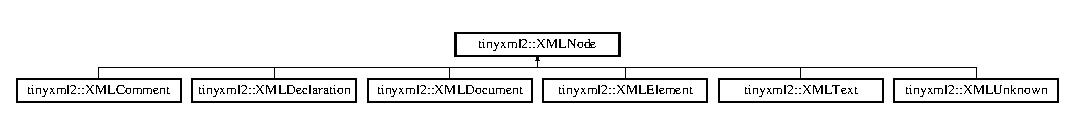
\includegraphics[height=1.145194cm]{classtinyxml2_1_1_x_m_l_node}
\end{center}
\end{figure}
\subsection*{Public Member Functions}
\begin{DoxyCompactItemize}
\item 
const \hyperlink{classtinyxml2_1_1_x_m_l_document}{X\+M\+L\+Document} $\ast$ \hyperlink{classtinyxml2_1_1_x_m_l_node_add244bca368083fa29698db8dcf147ca}{Get\+Document} () const \hypertarget{classtinyxml2_1_1_x_m_l_node_add244bca368083fa29698db8dcf147ca}{}\label{classtinyxml2_1_1_x_m_l_node_add244bca368083fa29698db8dcf147ca}

\begin{DoxyCompactList}\small\item\em Get the \hyperlink{classtinyxml2_1_1_x_m_l_document}{X\+M\+L\+Document} that owns this \hyperlink{classtinyxml2_1_1_x_m_l_node}{X\+M\+L\+Node}. \end{DoxyCompactList}\item 
\hyperlink{classtinyxml2_1_1_x_m_l_document}{X\+M\+L\+Document} $\ast$ \hyperlink{classtinyxml2_1_1_x_m_l_node_af343d1ef0b45c0020e62d784d7e67a68}{Get\+Document} ()\hypertarget{classtinyxml2_1_1_x_m_l_node_af343d1ef0b45c0020e62d784d7e67a68}{}\label{classtinyxml2_1_1_x_m_l_node_af343d1ef0b45c0020e62d784d7e67a68}

\begin{DoxyCompactList}\small\item\em Get the \hyperlink{classtinyxml2_1_1_x_m_l_document}{X\+M\+L\+Document} that owns this \hyperlink{classtinyxml2_1_1_x_m_l_node}{X\+M\+L\+Node}. \end{DoxyCompactList}\item 
virtual \hyperlink{classtinyxml2_1_1_x_m_l_element}{X\+M\+L\+Element} $\ast$ \hyperlink{classtinyxml2_1_1_x_m_l_node_aab516e699567f75cc9ab2ef2eee501e8}{To\+Element} ()\hypertarget{classtinyxml2_1_1_x_m_l_node_aab516e699567f75cc9ab2ef2eee501e8}{}\label{classtinyxml2_1_1_x_m_l_node_aab516e699567f75cc9ab2ef2eee501e8}

\begin{DoxyCompactList}\small\item\em Safely cast to an Element, or null. \end{DoxyCompactList}\item 
virtual \hyperlink{classtinyxml2_1_1_x_m_l_text}{X\+M\+L\+Text} $\ast$ \hyperlink{classtinyxml2_1_1_x_m_l_node_a41c55dab9162d1eb62db2008430e376b}{To\+Text} ()\hypertarget{classtinyxml2_1_1_x_m_l_node_a41c55dab9162d1eb62db2008430e376b}{}\label{classtinyxml2_1_1_x_m_l_node_a41c55dab9162d1eb62db2008430e376b}

\begin{DoxyCompactList}\small\item\em Safely cast to Text, or null. \end{DoxyCompactList}\item 
virtual \hyperlink{classtinyxml2_1_1_x_m_l_comment}{X\+M\+L\+Comment} $\ast$ \hyperlink{classtinyxml2_1_1_x_m_l_node_aff47671055aa99840a1c1ebd661e63e3}{To\+Comment} ()\hypertarget{classtinyxml2_1_1_x_m_l_node_aff47671055aa99840a1c1ebd661e63e3}{}\label{classtinyxml2_1_1_x_m_l_node_aff47671055aa99840a1c1ebd661e63e3}

\begin{DoxyCompactList}\small\item\em Safely cast to a Comment, or null. \end{DoxyCompactList}\item 
virtual \hyperlink{classtinyxml2_1_1_x_m_l_document}{X\+M\+L\+Document} $\ast$ \hyperlink{classtinyxml2_1_1_x_m_l_node_a836e2966ed736fc3c94f70e12a2a3357}{To\+Document} ()\hypertarget{classtinyxml2_1_1_x_m_l_node_a836e2966ed736fc3c94f70e12a2a3357}{}\label{classtinyxml2_1_1_x_m_l_node_a836e2966ed736fc3c94f70e12a2a3357}

\begin{DoxyCompactList}\small\item\em Safely cast to a Document, or null. \end{DoxyCompactList}\item 
virtual \hyperlink{classtinyxml2_1_1_x_m_l_declaration}{X\+M\+L\+Declaration} $\ast$ \hyperlink{classtinyxml2_1_1_x_m_l_node_a174fd4c22c010b58138c1b84a0dfbd51}{To\+Declaration} ()\hypertarget{classtinyxml2_1_1_x_m_l_node_a174fd4c22c010b58138c1b84a0dfbd51}{}\label{classtinyxml2_1_1_x_m_l_node_a174fd4c22c010b58138c1b84a0dfbd51}

\begin{DoxyCompactList}\small\item\em Safely cast to a Declaration, or null. \end{DoxyCompactList}\item 
virtual \hyperlink{classtinyxml2_1_1_x_m_l_unknown}{X\+M\+L\+Unknown} $\ast$ \hyperlink{classtinyxml2_1_1_x_m_l_node_a8675a74aa0ada6eccab0c77ef3e5b9bd}{To\+Unknown} ()\hypertarget{classtinyxml2_1_1_x_m_l_node_a8675a74aa0ada6eccab0c77ef3e5b9bd}{}\label{classtinyxml2_1_1_x_m_l_node_a8675a74aa0ada6eccab0c77ef3e5b9bd}

\begin{DoxyCompactList}\small\item\em Safely cast to an Unknown, or null. \end{DoxyCompactList}\item 
virtual const \hyperlink{classtinyxml2_1_1_x_m_l_element}{X\+M\+L\+Element} $\ast$ {\bfseries To\+Element} () const \hypertarget{classtinyxml2_1_1_x_m_l_node_acbaec609797ddabb4f9dcf38ee91262e}{}\label{classtinyxml2_1_1_x_m_l_node_acbaec609797ddabb4f9dcf38ee91262e}

\item 
virtual const \hyperlink{classtinyxml2_1_1_x_m_l_text}{X\+M\+L\+Text} $\ast$ {\bfseries To\+Text} () const \hypertarget{classtinyxml2_1_1_x_m_l_node_a89009ffc1b9f5d692bf8d4c9f18c3bec}{}\label{classtinyxml2_1_1_x_m_l_node_a89009ffc1b9f5d692bf8d4c9f18c3bec}

\item 
virtual const \hyperlink{classtinyxml2_1_1_x_m_l_comment}{X\+M\+L\+Comment} $\ast$ {\bfseries To\+Comment} () const \hypertarget{classtinyxml2_1_1_x_m_l_node_a157ce3a00ea5ee5a85b7103138e85e8a}{}\label{classtinyxml2_1_1_x_m_l_node_a157ce3a00ea5ee5a85b7103138e85e8a}

\item 
virtual const \hyperlink{classtinyxml2_1_1_x_m_l_document}{X\+M\+L\+Document} $\ast$ {\bfseries To\+Document} () const \hypertarget{classtinyxml2_1_1_x_m_l_node_a3ff975733a17d6ced3539b45544c8bf6}{}\label{classtinyxml2_1_1_x_m_l_node_a3ff975733a17d6ced3539b45544c8bf6}

\item 
virtual const \hyperlink{classtinyxml2_1_1_x_m_l_declaration}{X\+M\+L\+Declaration} $\ast$ {\bfseries To\+Declaration} () const \hypertarget{classtinyxml2_1_1_x_m_l_node_aedae0bbb58d533a4b8a61042388b49e5}{}\label{classtinyxml2_1_1_x_m_l_node_aedae0bbb58d533a4b8a61042388b49e5}

\item 
virtual const \hyperlink{classtinyxml2_1_1_x_m_l_unknown}{X\+M\+L\+Unknown} $\ast$ {\bfseries To\+Unknown} () const \hypertarget{classtinyxml2_1_1_x_m_l_node_a71f5ae90296dbe67979f83fe97073efa}{}\label{classtinyxml2_1_1_x_m_l_node_a71f5ae90296dbe67979f83fe97073efa}

\item 
const char $\ast$ \hyperlink{classtinyxml2_1_1_x_m_l_node_a92835c779871918f9af569bfe9669fe6}{Value} () const 
\item 
void \hyperlink{classtinyxml2_1_1_x_m_l_node_a09dd68cf9eae137579f6e50f36487513}{Set\+Value} (const char $\ast$val, bool static\+Mem=false)
\item 
const \hyperlink{classtinyxml2_1_1_x_m_l_node}{X\+M\+L\+Node} $\ast$ \hyperlink{classtinyxml2_1_1_x_m_l_node_a4e39bdcf9bfafa55d04857ece6aaf64e}{Parent} () const \hypertarget{classtinyxml2_1_1_x_m_l_node_a4e39bdcf9bfafa55d04857ece6aaf64e}{}\label{classtinyxml2_1_1_x_m_l_node_a4e39bdcf9bfafa55d04857ece6aaf64e}

\begin{DoxyCompactList}\small\item\em Get the parent of this node on the D\+OM. \end{DoxyCompactList}\item 
\hyperlink{classtinyxml2_1_1_x_m_l_node}{X\+M\+L\+Node} $\ast$ {\bfseries Parent} ()\hypertarget{classtinyxml2_1_1_x_m_l_node_a76029693a5a54fbb721a41d7a0ca8a97}{}\label{classtinyxml2_1_1_x_m_l_node_a76029693a5a54fbb721a41d7a0ca8a97}

\item 
bool \hyperlink{classtinyxml2_1_1_x_m_l_node_a96afe34a9ccd0ed4c0cff32beb42cc6c}{No\+Children} () const \hypertarget{classtinyxml2_1_1_x_m_l_node_a96afe34a9ccd0ed4c0cff32beb42cc6c}{}\label{classtinyxml2_1_1_x_m_l_node_a96afe34a9ccd0ed4c0cff32beb42cc6c}

\begin{DoxyCompactList}\small\item\em Returns true if this node has no children. \end{DoxyCompactList}\item 
const \hyperlink{classtinyxml2_1_1_x_m_l_node}{X\+M\+L\+Node} $\ast$ \hyperlink{classtinyxml2_1_1_x_m_l_node_a60e923d13d7dc01f45ab90a2f948b02a}{First\+Child} () const \hypertarget{classtinyxml2_1_1_x_m_l_node_a60e923d13d7dc01f45ab90a2f948b02a}{}\label{classtinyxml2_1_1_x_m_l_node_a60e923d13d7dc01f45ab90a2f948b02a}

\begin{DoxyCompactList}\small\item\em Get the first child node, or null if none exists. \end{DoxyCompactList}\item 
\hyperlink{classtinyxml2_1_1_x_m_l_node}{X\+M\+L\+Node} $\ast$ {\bfseries First\+Child} ()\hypertarget{classtinyxml2_1_1_x_m_l_node_a2d6c70c475146b48bc93a7fafdeff5e0}{}\label{classtinyxml2_1_1_x_m_l_node_a2d6c70c475146b48bc93a7fafdeff5e0}

\item 
const \hyperlink{classtinyxml2_1_1_x_m_l_element}{X\+M\+L\+Element} $\ast$ \hyperlink{classtinyxml2_1_1_x_m_l_node_a4a38e0da23f4d97673a86c77d5cae5c2}{First\+Child\+Element} (const char $\ast$name=0) const 
\item 
\hyperlink{classtinyxml2_1_1_x_m_l_element}{X\+M\+L\+Element} $\ast$ {\bfseries First\+Child\+Element} (const char $\ast$name=0)\hypertarget{classtinyxml2_1_1_x_m_l_node_af1e0e475cc27d5e7eeaf4d732691b741}{}\label{classtinyxml2_1_1_x_m_l_node_af1e0e475cc27d5e7eeaf4d732691b741}

\item 
const \hyperlink{classtinyxml2_1_1_x_m_l_node}{X\+M\+L\+Node} $\ast$ \hyperlink{classtinyxml2_1_1_x_m_l_node_a6088246532b02895beb0e6fa561a7f3b}{Last\+Child} () const \hypertarget{classtinyxml2_1_1_x_m_l_node_a6088246532b02895beb0e6fa561a7f3b}{}\label{classtinyxml2_1_1_x_m_l_node_a6088246532b02895beb0e6fa561a7f3b}

\begin{DoxyCompactList}\small\item\em Get the last child node, or null if none exists. \end{DoxyCompactList}\item 
\hyperlink{classtinyxml2_1_1_x_m_l_node}{X\+M\+L\+Node} $\ast$ {\bfseries Last\+Child} ()\hypertarget{classtinyxml2_1_1_x_m_l_node_ad7552c8cb1dc0cb6f3bdc14a9d115dbf}{}\label{classtinyxml2_1_1_x_m_l_node_ad7552c8cb1dc0cb6f3bdc14a9d115dbf}

\item 
const \hyperlink{classtinyxml2_1_1_x_m_l_element}{X\+M\+L\+Element} $\ast$ \hyperlink{classtinyxml2_1_1_x_m_l_node_a91a59df4ae1b4eb7f573c0a4cfc81bee}{Last\+Child\+Element} (const char $\ast$name=0) const 
\item 
\hyperlink{classtinyxml2_1_1_x_m_l_element}{X\+M\+L\+Element} $\ast$ {\bfseries Last\+Child\+Element} (const char $\ast$name=0)\hypertarget{classtinyxml2_1_1_x_m_l_node_a1b77a8194d059665a4412ebfea276878}{}\label{classtinyxml2_1_1_x_m_l_node_a1b77a8194d059665a4412ebfea276878}

\item 
const \hyperlink{classtinyxml2_1_1_x_m_l_node}{X\+M\+L\+Node} $\ast$ \hyperlink{classtinyxml2_1_1_x_m_l_node_a4cb1bf63e9de55129d21a7be60685fd4}{Previous\+Sibling} () const \hypertarget{classtinyxml2_1_1_x_m_l_node_a4cb1bf63e9de55129d21a7be60685fd4}{}\label{classtinyxml2_1_1_x_m_l_node_a4cb1bf63e9de55129d21a7be60685fd4}

\begin{DoxyCompactList}\small\item\em Get the previous (left) sibling node of this node. \end{DoxyCompactList}\item 
\hyperlink{classtinyxml2_1_1_x_m_l_node}{X\+M\+L\+Node} $\ast$ {\bfseries Previous\+Sibling} ()\hypertarget{classtinyxml2_1_1_x_m_l_node_ae760e5e7e766df1d2cf3bb4a847876d6}{}\label{classtinyxml2_1_1_x_m_l_node_ae760e5e7e766df1d2cf3bb4a847876d6}

\item 
const \hyperlink{classtinyxml2_1_1_x_m_l_element}{X\+M\+L\+Element} $\ast$ \hyperlink{classtinyxml2_1_1_x_m_l_node_aae864cedca1b711cf0e357fd6504a6d8}{Previous\+Sibling\+Element} (const char $\ast$name=0) const \hypertarget{classtinyxml2_1_1_x_m_l_node_aae864cedca1b711cf0e357fd6504a6d8}{}\label{classtinyxml2_1_1_x_m_l_node_aae864cedca1b711cf0e357fd6504a6d8}

\begin{DoxyCompactList}\small\item\em Get the previous (left) sibling element of this node, with an optionally supplied name. \end{DoxyCompactList}\item 
\hyperlink{classtinyxml2_1_1_x_m_l_element}{X\+M\+L\+Element} $\ast$ {\bfseries Previous\+Sibling\+Element} (const char $\ast$name=0)\hypertarget{classtinyxml2_1_1_x_m_l_node_ae4f37eb6cd405bdf1d57caa066e36d87}{}\label{classtinyxml2_1_1_x_m_l_node_ae4f37eb6cd405bdf1d57caa066e36d87}

\item 
const \hyperlink{classtinyxml2_1_1_x_m_l_node}{X\+M\+L\+Node} $\ast$ \hyperlink{classtinyxml2_1_1_x_m_l_node_abba1df37581d89dccc45acdc55750ba2}{Next\+Sibling} () const \hypertarget{classtinyxml2_1_1_x_m_l_node_abba1df37581d89dccc45acdc55750ba2}{}\label{classtinyxml2_1_1_x_m_l_node_abba1df37581d89dccc45acdc55750ba2}

\begin{DoxyCompactList}\small\item\em Get the next (right) sibling node of this node. \end{DoxyCompactList}\item 
\hyperlink{classtinyxml2_1_1_x_m_l_node}{X\+M\+L\+Node} $\ast$ {\bfseries Next\+Sibling} ()\hypertarget{classtinyxml2_1_1_x_m_l_node_aeb7d4dfd8fb924ef86e7cb72183acbac}{}\label{classtinyxml2_1_1_x_m_l_node_aeb7d4dfd8fb924ef86e7cb72183acbac}

\item 
const \hyperlink{classtinyxml2_1_1_x_m_l_element}{X\+M\+L\+Element} $\ast$ \hyperlink{classtinyxml2_1_1_x_m_l_node_ab66a0818d72cee86e0952ed2da701f8b}{Next\+Sibling\+Element} (const char $\ast$name=0) const \hypertarget{classtinyxml2_1_1_x_m_l_node_ab66a0818d72cee86e0952ed2da701f8b}{}\label{classtinyxml2_1_1_x_m_l_node_ab66a0818d72cee86e0952ed2da701f8b}

\begin{DoxyCompactList}\small\item\em Get the next (right) sibling element of this node, with an optionally supplied name. \end{DoxyCompactList}\item 
\hyperlink{classtinyxml2_1_1_x_m_l_element}{X\+M\+L\+Element} $\ast$ {\bfseries Next\+Sibling\+Element} (const char $\ast$name=0)\hypertarget{classtinyxml2_1_1_x_m_l_node_af1225412584d4a2126f55e96a12e0ec0}{}\label{classtinyxml2_1_1_x_m_l_node_af1225412584d4a2126f55e96a12e0ec0}

\item 
\hyperlink{classtinyxml2_1_1_x_m_l_node}{X\+M\+L\+Node} $\ast$ \hyperlink{classtinyxml2_1_1_x_m_l_node_ae3b422e98914d6002ca99bb1d2837103}{Insert\+End\+Child} (\hyperlink{classtinyxml2_1_1_x_m_l_node}{X\+M\+L\+Node} $\ast$add\+This)
\item 
\hyperlink{classtinyxml2_1_1_x_m_l_node}{X\+M\+L\+Node} $\ast$ {\bfseries Link\+End\+Child} (\hyperlink{classtinyxml2_1_1_x_m_l_node}{X\+M\+L\+Node} $\ast$add\+This)\hypertarget{classtinyxml2_1_1_x_m_l_node_a663e3a5a378169fd477378f4d17a7649}{}\label{classtinyxml2_1_1_x_m_l_node_a663e3a5a378169fd477378f4d17a7649}

\item 
\hyperlink{classtinyxml2_1_1_x_m_l_node}{X\+M\+L\+Node} $\ast$ \hyperlink{classtinyxml2_1_1_x_m_l_node_ac609a8f3ea949027f439280c640bbaf2}{Insert\+First\+Child} (\hyperlink{classtinyxml2_1_1_x_m_l_node}{X\+M\+L\+Node} $\ast$add\+This)
\item 
\hyperlink{classtinyxml2_1_1_x_m_l_node}{X\+M\+L\+Node} $\ast$ \hyperlink{classtinyxml2_1_1_x_m_l_node_a9275138a1b8dd5d8e2c26789bdc23ac8}{Insert\+After\+Child} (\hyperlink{classtinyxml2_1_1_x_m_l_node}{X\+M\+L\+Node} $\ast$after\+This, \hyperlink{classtinyxml2_1_1_x_m_l_node}{X\+M\+L\+Node} $\ast$add\+This)
\item 
void \hyperlink{classtinyxml2_1_1_x_m_l_node_a0360085cc54df5bff85d5c5da13afdce}{Delete\+Children} ()
\item 
void \hyperlink{classtinyxml2_1_1_x_m_l_node_a363b6edbd6ebd55f8387d2b89f2b0921}{Delete\+Child} (\hyperlink{classtinyxml2_1_1_x_m_l_node}{X\+M\+L\+Node} $\ast$node)
\item 
virtual \hyperlink{classtinyxml2_1_1_x_m_l_node}{X\+M\+L\+Node} $\ast$ \hyperlink{classtinyxml2_1_1_x_m_l_node_a83e3524e2ecea25eeab630c7ab113627}{Shallow\+Clone} (\hyperlink{classtinyxml2_1_1_x_m_l_document}{X\+M\+L\+Document} $\ast$document) const  =0
\item 
virtual bool \hyperlink{classtinyxml2_1_1_x_m_l_node_ac50408e91e095237f45716092ac2bddc}{Shallow\+Equal} (const \hyperlink{classtinyxml2_1_1_x_m_l_node}{X\+M\+L\+Node} $\ast$compare) const  =0
\item 
virtual bool \hyperlink{classtinyxml2_1_1_x_m_l_node_a366ad0e9b9ae8d1b18c00f903994b7a9}{Accept} (\hyperlink{classtinyxml2_1_1_x_m_l_visitor}{X\+M\+L\+Visitor} $\ast$visitor) const  =0
\end{DoxyCompactItemize}
\subsection*{Protected Member Functions}
\begin{DoxyCompactItemize}
\item 
{\bfseries X\+M\+L\+Node} (\hyperlink{classtinyxml2_1_1_x_m_l_document}{X\+M\+L\+Document} $\ast$)\hypertarget{classtinyxml2_1_1_x_m_l_node_a29868df6ca383d574f584dfdd15105b6}{}\label{classtinyxml2_1_1_x_m_l_node_a29868df6ca383d574f584dfdd15105b6}

\item 
virtual char $\ast$ {\bfseries Parse\+Deep} (char $\ast$, \hyperlink{classtinyxml2_1_1_str_pair}{Str\+Pair} $\ast$)\hypertarget{classtinyxml2_1_1_x_m_l_node_a7610d0f603e8b603d2078521811a23c1}{}\label{classtinyxml2_1_1_x_m_l_node_a7610d0f603e8b603d2078521811a23c1}

\end{DoxyCompactItemize}
\subsection*{Protected Attributes}
\begin{DoxyCompactItemize}
\item 
\hyperlink{classtinyxml2_1_1_x_m_l_document}{X\+M\+L\+Document} $\ast$ {\bfseries \+\_\+document}\hypertarget{classtinyxml2_1_1_x_m_l_node_a8d2d2be0bb6797625551eb0e91f0ff62}{}\label{classtinyxml2_1_1_x_m_l_node_a8d2d2be0bb6797625551eb0e91f0ff62}

\item 
\hyperlink{classtinyxml2_1_1_x_m_l_node}{X\+M\+L\+Node} $\ast$ {\bfseries \+\_\+parent}\hypertarget{classtinyxml2_1_1_x_m_l_node_a176dd1c4965c21c366de192164aa2c13}{}\label{classtinyxml2_1_1_x_m_l_node_a176dd1c4965c21c366de192164aa2c13}

\item 
\hyperlink{classtinyxml2_1_1_str_pair}{Str\+Pair} {\bfseries \+\_\+value}\hypertarget{classtinyxml2_1_1_x_m_l_node_a3ea9884098b8379de2bb5ab3fc85c0fc}{}\label{classtinyxml2_1_1_x_m_l_node_a3ea9884098b8379de2bb5ab3fc85c0fc}

\item 
\hyperlink{classtinyxml2_1_1_x_m_l_node}{X\+M\+L\+Node} $\ast$ {\bfseries \+\_\+first\+Child}\hypertarget{classtinyxml2_1_1_x_m_l_node_aa20c91e4213dc930c5bdf420322ca342}{}\label{classtinyxml2_1_1_x_m_l_node_aa20c91e4213dc930c5bdf420322ca342}

\item 
\hyperlink{classtinyxml2_1_1_x_m_l_node}{X\+M\+L\+Node} $\ast$ {\bfseries \+\_\+last\+Child}\hypertarget{classtinyxml2_1_1_x_m_l_node_a099b6560ae44ab9edb8453aaf1a3747b}{}\label{classtinyxml2_1_1_x_m_l_node_a099b6560ae44ab9edb8453aaf1a3747b}

\item 
\hyperlink{classtinyxml2_1_1_x_m_l_node}{X\+M\+L\+Node} $\ast$ {\bfseries \+\_\+prev}\hypertarget{classtinyxml2_1_1_x_m_l_node_a9739eb0fb9a1188266052055e7a6bf6b}{}\label{classtinyxml2_1_1_x_m_l_node_a9739eb0fb9a1188266052055e7a6bf6b}

\item 
\hyperlink{classtinyxml2_1_1_x_m_l_node}{X\+M\+L\+Node} $\ast$ {\bfseries \+\_\+next}\hypertarget{classtinyxml2_1_1_x_m_l_node_a27e985496b37dd00eb5b9cf59b9e3fb1}{}\label{classtinyxml2_1_1_x_m_l_node_a27e985496b37dd00eb5b9cf59b9e3fb1}

\end{DoxyCompactItemize}
\subsection*{Friends}
\begin{DoxyCompactItemize}
\item 
class {\bfseries X\+M\+L\+Document}\hypertarget{classtinyxml2_1_1_x_m_l_node_a4eee3bda60c60a30e4e8cd4ea91c4c6e}{}\label{classtinyxml2_1_1_x_m_l_node_a4eee3bda60c60a30e4e8cd4ea91c4c6e}

\item 
class {\bfseries X\+M\+L\+Element}\hypertarget{classtinyxml2_1_1_x_m_l_node_ac2fba9b6e452829dd892f7392c24e0eb}{}\label{classtinyxml2_1_1_x_m_l_node_ac2fba9b6e452829dd892f7392c24e0eb}

\end{DoxyCompactItemize}


\subsection{Detailed Description}
\hyperlink{classtinyxml2_1_1_x_m_l_node}{X\+M\+L\+Node} is a base class for every object that is in the X\+ML Document \hyperlink{class_object}{Object} Model (D\+OM), except X\+M\+L\+Attributes. Nodes have siblings, a parent, and children which can be navigated. A node is always in a \hyperlink{classtinyxml2_1_1_x_m_l_document}{X\+M\+L\+Document}. The type of a \hyperlink{classtinyxml2_1_1_x_m_l_node}{X\+M\+L\+Node} can be queried, and it can be cast to its more defined type.

A \hyperlink{classtinyxml2_1_1_x_m_l_document}{X\+M\+L\+Document} allocates memory for all its Nodes. When the \hyperlink{classtinyxml2_1_1_x_m_l_document}{X\+M\+L\+Document} gets deleted, all its Nodes will also be deleted.

\begin{DoxyVerb}A Document can contain: Element (container or leaf)
                        Comment (leaf)
                        Unknown (leaf)
                        Declaration( leaf )

An Element can contain: Element (container or leaf)
                        Text    (leaf)
                        Attributes (not on tree)
                        Comment (leaf)
                        Unknown (leaf)\end{DoxyVerb}
 

\subsection{Member Function Documentation}
\index{tinyxml2\+::\+X\+M\+L\+Node@{tinyxml2\+::\+X\+M\+L\+Node}!Accept@{Accept}}
\index{Accept@{Accept}!tinyxml2\+::\+X\+M\+L\+Node@{tinyxml2\+::\+X\+M\+L\+Node}}
\subsubsection[{\texorpdfstring{Accept(\+X\+M\+L\+Visitor $\ast$visitor) const  =0}{Accept(XMLVisitor *visitor) const  =0}}]{\setlength{\rightskip}{0pt plus 5cm}virtual bool tinyxml2\+::\+X\+M\+L\+Node\+::\+Accept (
\begin{DoxyParamCaption}
\item[{{\bf X\+M\+L\+Visitor} $\ast$}]{visitor}
\end{DoxyParamCaption}
) const\hspace{0.3cm}{\ttfamily [pure virtual]}}\hypertarget{classtinyxml2_1_1_x_m_l_node_a366ad0e9b9ae8d1b18c00f903994b7a9}{}\label{classtinyxml2_1_1_x_m_l_node_a366ad0e9b9ae8d1b18c00f903994b7a9}
Accept a hierarchical visit of the nodes in the Tiny\+X\+M\+L-\/2 D\+OM. Every node in the X\+ML tree will be conditionally visited and the host will be called back via the \hyperlink{classtinyxml2_1_1_x_m_l_visitor}{X\+M\+L\+Visitor} interface.

This is essentially a S\+AX interface for Tiny\+X\+M\+L-\/2. (Note however it doesn\textquotesingle{}t re-\/parse the X\+ML for the callbacks, so the performance of Tiny\+X\+M\+L-\/2 is unchanged by using this interface versus any other.)

The interface has been based on ideas from\+:


\begin{DoxyItemize}
\item \href{http://www.saxproject.org/}{\tt http\+://www.\+saxproject.\+org/}
\item \href{http://c2.com/cgi/wiki?HierarchicalVisitorPattern}{\tt http\+://c2.\+com/cgi/wiki?\+Hierarchical\+Visitor\+Pattern}
\end{DoxyItemize}

Which are both good references for \char`\"{}visiting\char`\"{}.

An example of using \hyperlink{classtinyxml2_1_1_x_m_l_node_a366ad0e9b9ae8d1b18c00f903994b7a9}{Accept()}\+: \begin{DoxyVerb}XMLPrinter printer;
tinyxmlDoc.Accept( &printer );
const char* xmlcstr = printer.CStr();
\end{DoxyVerb}
 

Implemented in \hyperlink{classtinyxml2_1_1_x_m_l_document_aa08503d24898bf9992ae5e5fb8b0cf87}{tinyxml2\+::\+X\+M\+L\+Document}, \hyperlink{classtinyxml2_1_1_x_m_l_element_a36d65438991a1e85096caf39ad13a099}{tinyxml2\+::\+X\+M\+L\+Element}, \hyperlink{classtinyxml2_1_1_x_m_l_unknown_a0d341ab804a1438a474810bb5bd29dd5}{tinyxml2\+::\+X\+M\+L\+Unknown}, \hyperlink{classtinyxml2_1_1_x_m_l_declaration_a953a7359cc312d15218eb5843a4ca108}{tinyxml2\+::\+X\+M\+L\+Declaration}, \hyperlink{classtinyxml2_1_1_x_m_l_comment_aa382b1be6a8b0650c16a2d88bb499335}{tinyxml2\+::\+X\+M\+L\+Comment}, and \hyperlink{classtinyxml2_1_1_x_m_l_text_ae659d4fc7351a7df11c111cbe1ade46f}{tinyxml2\+::\+X\+M\+L\+Text}.

\index{tinyxml2\+::\+X\+M\+L\+Node@{tinyxml2\+::\+X\+M\+L\+Node}!Delete\+Child@{Delete\+Child}}
\index{Delete\+Child@{Delete\+Child}!tinyxml2\+::\+X\+M\+L\+Node@{tinyxml2\+::\+X\+M\+L\+Node}}
\subsubsection[{\texorpdfstring{Delete\+Child(\+X\+M\+L\+Node $\ast$node)}{DeleteChild(XMLNode *node)}}]{\setlength{\rightskip}{0pt plus 5cm}void tinyxml2\+::\+X\+M\+L\+Node\+::\+Delete\+Child (
\begin{DoxyParamCaption}
\item[{{\bf X\+M\+L\+Node} $\ast$}]{node}
\end{DoxyParamCaption}
)}\hypertarget{classtinyxml2_1_1_x_m_l_node_a363b6edbd6ebd55f8387d2b89f2b0921}{}\label{classtinyxml2_1_1_x_m_l_node_a363b6edbd6ebd55f8387d2b89f2b0921}
Delete a child of this node. \index{tinyxml2\+::\+X\+M\+L\+Node@{tinyxml2\+::\+X\+M\+L\+Node}!Delete\+Children@{Delete\+Children}}
\index{Delete\+Children@{Delete\+Children}!tinyxml2\+::\+X\+M\+L\+Node@{tinyxml2\+::\+X\+M\+L\+Node}}
\subsubsection[{\texorpdfstring{Delete\+Children()}{DeleteChildren()}}]{\setlength{\rightskip}{0pt plus 5cm}void tinyxml2\+::\+X\+M\+L\+Node\+::\+Delete\+Children (
\begin{DoxyParamCaption}
{}
\end{DoxyParamCaption}
)}\hypertarget{classtinyxml2_1_1_x_m_l_node_a0360085cc54df5bff85d5c5da13afdce}{}\label{classtinyxml2_1_1_x_m_l_node_a0360085cc54df5bff85d5c5da13afdce}
Delete all the children of this node. \index{tinyxml2\+::\+X\+M\+L\+Node@{tinyxml2\+::\+X\+M\+L\+Node}!First\+Child\+Element@{First\+Child\+Element}}
\index{First\+Child\+Element@{First\+Child\+Element}!tinyxml2\+::\+X\+M\+L\+Node@{tinyxml2\+::\+X\+M\+L\+Node}}
\subsubsection[{\texorpdfstring{First\+Child\+Element(const char $\ast$name=0) const }{FirstChildElement(const char *name=0) const }}]{\setlength{\rightskip}{0pt plus 5cm}const {\bf X\+M\+L\+Element} $\ast$ tinyxml2\+::\+X\+M\+L\+Node\+::\+First\+Child\+Element (
\begin{DoxyParamCaption}
\item[{const char $\ast$}]{name = {\ttfamily 0}}
\end{DoxyParamCaption}
) const}\hypertarget{classtinyxml2_1_1_x_m_l_node_a4a38e0da23f4d97673a86c77d5cae5c2}{}\label{classtinyxml2_1_1_x_m_l_node_a4a38e0da23f4d97673a86c77d5cae5c2}
Get the first child element, or optionally the first child element with the specified name. \index{tinyxml2\+::\+X\+M\+L\+Node@{tinyxml2\+::\+X\+M\+L\+Node}!Insert\+After\+Child@{Insert\+After\+Child}}
\index{Insert\+After\+Child@{Insert\+After\+Child}!tinyxml2\+::\+X\+M\+L\+Node@{tinyxml2\+::\+X\+M\+L\+Node}}
\subsubsection[{\texorpdfstring{Insert\+After\+Child(\+X\+M\+L\+Node $\ast$after\+This, X\+M\+L\+Node $\ast$add\+This)}{InsertAfterChild(XMLNode *afterThis, XMLNode *addThis)}}]{\setlength{\rightskip}{0pt plus 5cm}{\bf X\+M\+L\+Node} $\ast$ tinyxml2\+::\+X\+M\+L\+Node\+::\+Insert\+After\+Child (
\begin{DoxyParamCaption}
\item[{{\bf X\+M\+L\+Node} $\ast$}]{after\+This, }
\item[{{\bf X\+M\+L\+Node} $\ast$}]{add\+This}
\end{DoxyParamCaption}
)}\hypertarget{classtinyxml2_1_1_x_m_l_node_a9275138a1b8dd5d8e2c26789bdc23ac8}{}\label{classtinyxml2_1_1_x_m_l_node_a9275138a1b8dd5d8e2c26789bdc23ac8}
Add a node after the specified child node. If the child node is already part of the document, it is moved from its old location to the new location. Returns the add\+This argument or 0 if the after\+This node is not a child of this node, or if the node does not belong to the same document. \index{tinyxml2\+::\+X\+M\+L\+Node@{tinyxml2\+::\+X\+M\+L\+Node}!Insert\+End\+Child@{Insert\+End\+Child}}
\index{Insert\+End\+Child@{Insert\+End\+Child}!tinyxml2\+::\+X\+M\+L\+Node@{tinyxml2\+::\+X\+M\+L\+Node}}
\subsubsection[{\texorpdfstring{Insert\+End\+Child(\+X\+M\+L\+Node $\ast$add\+This)}{InsertEndChild(XMLNode *addThis)}}]{\setlength{\rightskip}{0pt plus 5cm}{\bf X\+M\+L\+Node} $\ast$ tinyxml2\+::\+X\+M\+L\+Node\+::\+Insert\+End\+Child (
\begin{DoxyParamCaption}
\item[{{\bf X\+M\+L\+Node} $\ast$}]{add\+This}
\end{DoxyParamCaption}
)}\hypertarget{classtinyxml2_1_1_x_m_l_node_ae3b422e98914d6002ca99bb1d2837103}{}\label{classtinyxml2_1_1_x_m_l_node_ae3b422e98914d6002ca99bb1d2837103}
Add a child node as the last (right) child. If the child node is already part of the document, it is moved from its old location to the new location. Returns the add\+This argument or 0 if the node does not belong to the same document. \index{tinyxml2\+::\+X\+M\+L\+Node@{tinyxml2\+::\+X\+M\+L\+Node}!Insert\+First\+Child@{Insert\+First\+Child}}
\index{Insert\+First\+Child@{Insert\+First\+Child}!tinyxml2\+::\+X\+M\+L\+Node@{tinyxml2\+::\+X\+M\+L\+Node}}
\subsubsection[{\texorpdfstring{Insert\+First\+Child(\+X\+M\+L\+Node $\ast$add\+This)}{InsertFirstChild(XMLNode *addThis)}}]{\setlength{\rightskip}{0pt plus 5cm}{\bf X\+M\+L\+Node} $\ast$ tinyxml2\+::\+X\+M\+L\+Node\+::\+Insert\+First\+Child (
\begin{DoxyParamCaption}
\item[{{\bf X\+M\+L\+Node} $\ast$}]{add\+This}
\end{DoxyParamCaption}
)}\hypertarget{classtinyxml2_1_1_x_m_l_node_ac609a8f3ea949027f439280c640bbaf2}{}\label{classtinyxml2_1_1_x_m_l_node_ac609a8f3ea949027f439280c640bbaf2}
Add a child node as the first (left) child. If the child node is already part of the document, it is moved from its old location to the new location. Returns the add\+This argument or 0 if the node does not belong to the same document. \index{tinyxml2\+::\+X\+M\+L\+Node@{tinyxml2\+::\+X\+M\+L\+Node}!Last\+Child\+Element@{Last\+Child\+Element}}
\index{Last\+Child\+Element@{Last\+Child\+Element}!tinyxml2\+::\+X\+M\+L\+Node@{tinyxml2\+::\+X\+M\+L\+Node}}
\subsubsection[{\texorpdfstring{Last\+Child\+Element(const char $\ast$name=0) const }{LastChildElement(const char *name=0) const }}]{\setlength{\rightskip}{0pt plus 5cm}const {\bf X\+M\+L\+Element} $\ast$ tinyxml2\+::\+X\+M\+L\+Node\+::\+Last\+Child\+Element (
\begin{DoxyParamCaption}
\item[{const char $\ast$}]{name = {\ttfamily 0}}
\end{DoxyParamCaption}
) const}\hypertarget{classtinyxml2_1_1_x_m_l_node_a91a59df4ae1b4eb7f573c0a4cfc81bee}{}\label{classtinyxml2_1_1_x_m_l_node_a91a59df4ae1b4eb7f573c0a4cfc81bee}
Get the last child element or optionally the last child element with the specified name. \index{tinyxml2\+::\+X\+M\+L\+Node@{tinyxml2\+::\+X\+M\+L\+Node}!Set\+Value@{Set\+Value}}
\index{Set\+Value@{Set\+Value}!tinyxml2\+::\+X\+M\+L\+Node@{tinyxml2\+::\+X\+M\+L\+Node}}
\subsubsection[{\texorpdfstring{Set\+Value(const char $\ast$val, bool static\+Mem=false)}{SetValue(const char *val, bool staticMem=false)}}]{\setlength{\rightskip}{0pt plus 5cm}void tinyxml2\+::\+X\+M\+L\+Node\+::\+Set\+Value (
\begin{DoxyParamCaption}
\item[{const char $\ast$}]{val, }
\item[{bool}]{static\+Mem = {\ttfamily false}}
\end{DoxyParamCaption}
)}\hypertarget{classtinyxml2_1_1_x_m_l_node_a09dd68cf9eae137579f6e50f36487513}{}\label{classtinyxml2_1_1_x_m_l_node_a09dd68cf9eae137579f6e50f36487513}
Set the Value of an X\+ML node. \begin{DoxySeeAlso}{See also}
\hyperlink{classtinyxml2_1_1_x_m_l_node_a92835c779871918f9af569bfe9669fe6}{Value()} 
\end{DoxySeeAlso}
\index{tinyxml2\+::\+X\+M\+L\+Node@{tinyxml2\+::\+X\+M\+L\+Node}!Shallow\+Clone@{Shallow\+Clone}}
\index{Shallow\+Clone@{Shallow\+Clone}!tinyxml2\+::\+X\+M\+L\+Node@{tinyxml2\+::\+X\+M\+L\+Node}}
\subsubsection[{\texorpdfstring{Shallow\+Clone(\+X\+M\+L\+Document $\ast$document) const  =0}{ShallowClone(XMLDocument *document) const  =0}}]{\setlength{\rightskip}{0pt plus 5cm}virtual {\bf X\+M\+L\+Node}$\ast$ tinyxml2\+::\+X\+M\+L\+Node\+::\+Shallow\+Clone (
\begin{DoxyParamCaption}
\item[{{\bf X\+M\+L\+Document} $\ast$}]{document}
\end{DoxyParamCaption}
) const\hspace{0.3cm}{\ttfamily [pure virtual]}}\hypertarget{classtinyxml2_1_1_x_m_l_node_a83e3524e2ecea25eeab630c7ab113627}{}\label{classtinyxml2_1_1_x_m_l_node_a83e3524e2ecea25eeab630c7ab113627}
Make a copy of this node, but not its children. You may pass in a Document pointer that will be the owner of the new Node. If the \textquotesingle{}document\textquotesingle{} is null, then the node returned will be allocated from the current Document. (this-\/$>$\hyperlink{classtinyxml2_1_1_x_m_l_node_af343d1ef0b45c0020e62d784d7e67a68}{Get\+Document()})

Note\+: if called on a \hyperlink{classtinyxml2_1_1_x_m_l_document}{X\+M\+L\+Document}, this will return null. 

Implemented in \hyperlink{classtinyxml2_1_1_x_m_l_document_a57c8511ed9f83aa3e20909a3db3f83d0}{tinyxml2\+::\+X\+M\+L\+Document}, \hyperlink{classtinyxml2_1_1_x_m_l_element_a85d85e32c18863fff1eeed53ae1ce23d}{tinyxml2\+::\+X\+M\+L\+Element}, \hyperlink{classtinyxml2_1_1_x_m_l_unknown_aa09fc7cb0cd64d6bb9c5ae00ffc549ec}{tinyxml2\+::\+X\+M\+L\+Unknown}, \hyperlink{classtinyxml2_1_1_x_m_l_declaration_a39458732ee6796cfc85dd35d3c488e0b}{tinyxml2\+::\+X\+M\+L\+Declaration}, \hyperlink{classtinyxml2_1_1_x_m_l_comment_a90bb60193a691b484f5e1b487857016d}{tinyxml2\+::\+X\+M\+L\+Comment}, and \hyperlink{classtinyxml2_1_1_x_m_l_text_af5115f8cc83de2947ed6a9d13e2f88c8}{tinyxml2\+::\+X\+M\+L\+Text}.

\index{tinyxml2\+::\+X\+M\+L\+Node@{tinyxml2\+::\+X\+M\+L\+Node}!Shallow\+Equal@{Shallow\+Equal}}
\index{Shallow\+Equal@{Shallow\+Equal}!tinyxml2\+::\+X\+M\+L\+Node@{tinyxml2\+::\+X\+M\+L\+Node}}
\subsubsection[{\texorpdfstring{Shallow\+Equal(const X\+M\+L\+Node $\ast$compare) const  =0}{ShallowEqual(const XMLNode *compare) const  =0}}]{\setlength{\rightskip}{0pt plus 5cm}virtual bool tinyxml2\+::\+X\+M\+L\+Node\+::\+Shallow\+Equal (
\begin{DoxyParamCaption}
\item[{const {\bf X\+M\+L\+Node} $\ast$}]{compare}
\end{DoxyParamCaption}
) const\hspace{0.3cm}{\ttfamily [pure virtual]}}\hypertarget{classtinyxml2_1_1_x_m_l_node_ac50408e91e095237f45716092ac2bddc}{}\label{classtinyxml2_1_1_x_m_l_node_ac50408e91e095237f45716092ac2bddc}
Test if 2 nodes are the same, but don\textquotesingle{}t test children. The 2 nodes do not need to be in the same Document.

Note\+: if called on a \hyperlink{classtinyxml2_1_1_x_m_l_document}{X\+M\+L\+Document}, this will return false. 

Implemented in \hyperlink{classtinyxml2_1_1_x_m_l_document_a12eac66c6e45d074d5cc47319868cd66}{tinyxml2\+::\+X\+M\+L\+Document}, \hyperlink{classtinyxml2_1_1_x_m_l_element_a25d51a2aad92625c78441457d58c85bc}{tinyxml2\+::\+X\+M\+L\+Element}, \hyperlink{classtinyxml2_1_1_x_m_l_unknown_a0169df157bf69a092b404ca49621ff1a}{tinyxml2\+::\+X\+M\+L\+Unknown}, \hyperlink{classtinyxml2_1_1_x_m_l_declaration_ace0d2d9bc1b63278bd5e984ebe0c7bd0}{tinyxml2\+::\+X\+M\+L\+Declaration}, \hyperlink{classtinyxml2_1_1_x_m_l_comment_a2d9f26757b0018fce933e74420cda22a}{tinyxml2\+::\+X\+M\+L\+Comment}, and \hyperlink{classtinyxml2_1_1_x_m_l_text_a1588aa5d23cb21eb31f36df0aaaa8d66}{tinyxml2\+::\+X\+M\+L\+Text}.

\index{tinyxml2\+::\+X\+M\+L\+Node@{tinyxml2\+::\+X\+M\+L\+Node}!Value@{Value}}
\index{Value@{Value}!tinyxml2\+::\+X\+M\+L\+Node@{tinyxml2\+::\+X\+M\+L\+Node}}
\subsubsection[{\texorpdfstring{Value() const }{Value() const }}]{\setlength{\rightskip}{0pt plus 5cm}const char $\ast$ tinyxml2\+::\+X\+M\+L\+Node\+::\+Value (
\begin{DoxyParamCaption}
{}
\end{DoxyParamCaption}
) const}\hypertarget{classtinyxml2_1_1_x_m_l_node_a92835c779871918f9af569bfe9669fe6}{}\label{classtinyxml2_1_1_x_m_l_node_a92835c779871918f9af569bfe9669fe6}
The meaning of \textquotesingle{}value\textquotesingle{} changes for the specific type. \begin{DoxyVerb}Document:   empty (NULL is returned, not an empty string)
Element:    name of the element
Comment:    the comment text
Unknown:    the tag contents
Text:       the text string
\end{DoxyVerb}
 

The documentation for this class was generated from the following files\+:\begin{DoxyCompactItemize}
\item 
src/tinyxml2.\+h\item 
src/tinyxml2.\+cpp\end{DoxyCompactItemize}

\hypertarget{classtinyxml2_1_1_x_m_l_printer}{}\section{tinyxml2\+:\+:X\+M\+L\+Printer Class Reference}
\label{classtinyxml2_1_1_x_m_l_printer}\index{tinyxml2\+::\+X\+M\+L\+Printer@{tinyxml2\+::\+X\+M\+L\+Printer}}


{\ttfamily \#include $<$tinyxml2.\+h$>$}

Inheritance diagram for tinyxml2\+:\+:X\+M\+L\+Printer\+:\begin{figure}[H]
\begin{center}
\leavevmode
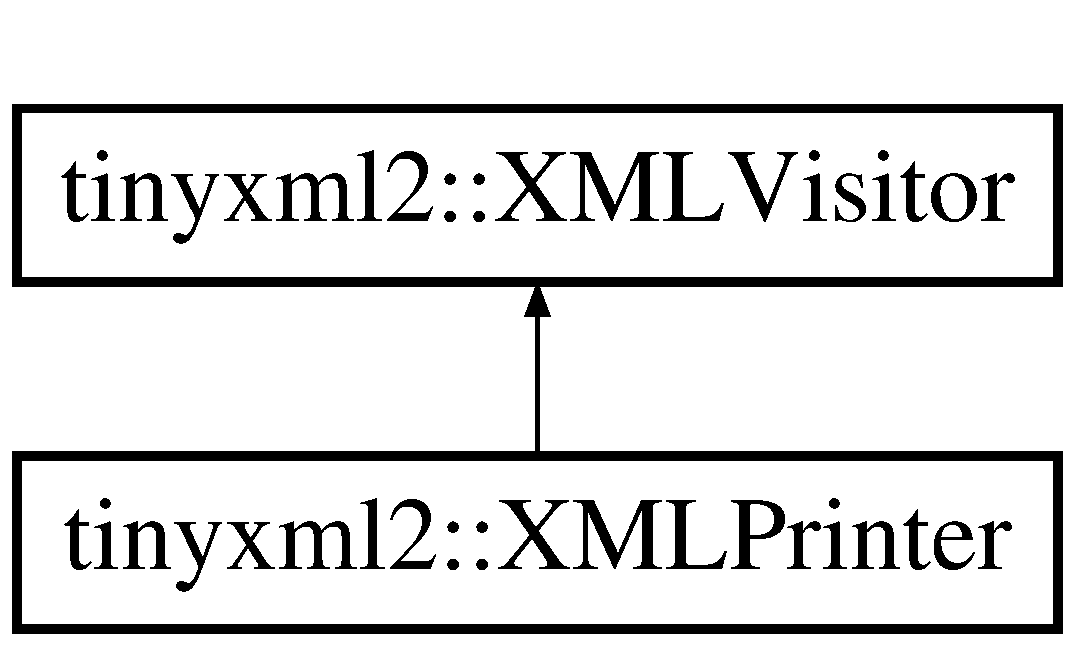
\includegraphics[height=2.000000cm]{classtinyxml2_1_1_x_m_l_printer}
\end{center}
\end{figure}
\subsection*{Public Member Functions}
\begin{DoxyCompactItemize}
\item 
\hyperlink{classtinyxml2_1_1_x_m_l_printer_aa6d3841c069085f5b8a27bc7103c04f7}{X\+M\+L\+Printer} (F\+I\+LE $\ast$file=0, bool compact=false, int depth=0)
\item 
void \hyperlink{classtinyxml2_1_1_x_m_l_printer_a178c608ce8476043d5d6513819cde903}{Push\+Header} (bool write\+B\+OM, bool write\+Declaration)
\item 
void \hyperlink{classtinyxml2_1_1_x_m_l_printer_a20fb06c83bd13e5140d7dd13af06c010}{Open\+Element} (const char $\ast$name, bool compact\+Mode=false)
\item 
void \hyperlink{classtinyxml2_1_1_x_m_l_printer_a9a4e2c9348b42e147629d5a99f4af3f0}{Push\+Attribute} (const char $\ast$name, const char $\ast$value)\hypertarget{classtinyxml2_1_1_x_m_l_printer_a9a4e2c9348b42e147629d5a99f4af3f0}{}\label{classtinyxml2_1_1_x_m_l_printer_a9a4e2c9348b42e147629d5a99f4af3f0}

\begin{DoxyCompactList}\small\item\em If streaming, add an attribute to an open element. \end{DoxyCompactList}\item 
void {\bfseries Push\+Attribute} (const char $\ast$name, int value)\hypertarget{classtinyxml2_1_1_x_m_l_printer_a69120c82088597372d28d0a98f2ee7a1}{}\label{classtinyxml2_1_1_x_m_l_printer_a69120c82088597372d28d0a98f2ee7a1}

\item 
void {\bfseries Push\+Attribute} (const char $\ast$name, unsigned value)\hypertarget{classtinyxml2_1_1_x_m_l_printer_aa41039e51990aaf5342f3e0575a692c4}{}\label{classtinyxml2_1_1_x_m_l_printer_aa41039e51990aaf5342f3e0575a692c4}

\item 
void {\bfseries Push\+Attribute} (const char $\ast$name, bool value)\hypertarget{classtinyxml2_1_1_x_m_l_printer_a51f7950d7b7a19f0d3a0d549a318d45f}{}\label{classtinyxml2_1_1_x_m_l_printer_a51f7950d7b7a19f0d3a0d549a318d45f}

\item 
void {\bfseries Push\+Attribute} (const char $\ast$name, double value)\hypertarget{classtinyxml2_1_1_x_m_l_printer_a1714867af40e68ca404c3e84b6cac2a6}{}\label{classtinyxml2_1_1_x_m_l_printer_a1714867af40e68ca404c3e84b6cac2a6}

\item 
virtual void \hyperlink{classtinyxml2_1_1_x_m_l_printer_af1fb439e5d800999646f333fa2f0699a}{Close\+Element} (bool compact\+Mode=false)\hypertarget{classtinyxml2_1_1_x_m_l_printer_af1fb439e5d800999646f333fa2f0699a}{}\label{classtinyxml2_1_1_x_m_l_printer_af1fb439e5d800999646f333fa2f0699a}

\begin{DoxyCompactList}\small\item\em If streaming, close the Element. \end{DoxyCompactList}\item 
void \hyperlink{classtinyxml2_1_1_x_m_l_printer_a1cc16a9362df4332012cb13cff6441b3}{Push\+Text} (const char $\ast$text, bool cdata=false)\hypertarget{classtinyxml2_1_1_x_m_l_printer_a1cc16a9362df4332012cb13cff6441b3}{}\label{classtinyxml2_1_1_x_m_l_printer_a1cc16a9362df4332012cb13cff6441b3}

\begin{DoxyCompactList}\small\item\em Add a text node. \end{DoxyCompactList}\item 
void \hyperlink{classtinyxml2_1_1_x_m_l_printer_a3e0d4d78de25d4cf081009e1431cea7e}{Push\+Text} (int value)\hypertarget{classtinyxml2_1_1_x_m_l_printer_a3e0d4d78de25d4cf081009e1431cea7e}{}\label{classtinyxml2_1_1_x_m_l_printer_a3e0d4d78de25d4cf081009e1431cea7e}

\begin{DoxyCompactList}\small\item\em Add a text node from an integer. \end{DoxyCompactList}\item 
void \hyperlink{classtinyxml2_1_1_x_m_l_printer_a661fb50e7e0a4918d2d259cb0fae647e}{Push\+Text} (unsigned value)\hypertarget{classtinyxml2_1_1_x_m_l_printer_a661fb50e7e0a4918d2d259cb0fae647e}{}\label{classtinyxml2_1_1_x_m_l_printer_a661fb50e7e0a4918d2d259cb0fae647e}

\begin{DoxyCompactList}\small\item\em Add a text node from an unsigned. \end{DoxyCompactList}\item 
void \hyperlink{classtinyxml2_1_1_x_m_l_printer_a4390e5fa1ed05189a8686647345ab29f}{Push\+Text} (bool value)\hypertarget{classtinyxml2_1_1_x_m_l_printer_a4390e5fa1ed05189a8686647345ab29f}{}\label{classtinyxml2_1_1_x_m_l_printer_a4390e5fa1ed05189a8686647345ab29f}

\begin{DoxyCompactList}\small\item\em Add a text node from a bool. \end{DoxyCompactList}\item 
void \hyperlink{classtinyxml2_1_1_x_m_l_printer_a1dbb1390e829d0673af66b9cd1928bd7}{Push\+Text} (float value)\hypertarget{classtinyxml2_1_1_x_m_l_printer_a1dbb1390e829d0673af66b9cd1928bd7}{}\label{classtinyxml2_1_1_x_m_l_printer_a1dbb1390e829d0673af66b9cd1928bd7}

\begin{DoxyCompactList}\small\item\em Add a text node from a float. \end{DoxyCompactList}\item 
void \hyperlink{classtinyxml2_1_1_x_m_l_printer_aa715302dfc09473c77c853cbd5431965}{Push\+Text} (double value)\hypertarget{classtinyxml2_1_1_x_m_l_printer_aa715302dfc09473c77c853cbd5431965}{}\label{classtinyxml2_1_1_x_m_l_printer_aa715302dfc09473c77c853cbd5431965}

\begin{DoxyCompactList}\small\item\em Add a text node from a double. \end{DoxyCompactList}\item 
void \hyperlink{classtinyxml2_1_1_x_m_l_printer_afc8416814219591c2fd5656e0c233140}{Push\+Comment} (const char $\ast$comment)\hypertarget{classtinyxml2_1_1_x_m_l_printer_afc8416814219591c2fd5656e0c233140}{}\label{classtinyxml2_1_1_x_m_l_printer_afc8416814219591c2fd5656e0c233140}

\begin{DoxyCompactList}\small\item\em Add a comment. \end{DoxyCompactList}\item 
void {\bfseries Push\+Declaration} (const char $\ast$value)\hypertarget{classtinyxml2_1_1_x_m_l_printer_a2fe3565e262594efc6c0276723c83fe7}{}\label{classtinyxml2_1_1_x_m_l_printer_a2fe3565e262594efc6c0276723c83fe7}

\item 
void {\bfseries Push\+Unknown} (const char $\ast$value)\hypertarget{classtinyxml2_1_1_x_m_l_printer_ab1efc6d1548505e9984185f58f54b713}{}\label{classtinyxml2_1_1_x_m_l_printer_ab1efc6d1548505e9984185f58f54b713}

\item 
virtual bool \hyperlink{classtinyxml2_1_1_x_m_l_printer_a9aa1de11a55a07db55a90fde37d7afad}{Visit\+Enter} (const \hyperlink{classtinyxml2_1_1_x_m_l_document}{X\+M\+L\+Document} \&)\hypertarget{classtinyxml2_1_1_x_m_l_printer_a9aa1de11a55a07db55a90fde37d7afad}{}\label{classtinyxml2_1_1_x_m_l_printer_a9aa1de11a55a07db55a90fde37d7afad}

\begin{DoxyCompactList}\small\item\em Visit a document. \end{DoxyCompactList}\item 
virtual bool \hyperlink{classtinyxml2_1_1_x_m_l_printer_a15fc1f2b922f540917dcf52808737b29}{Visit\+Exit} (const \hyperlink{classtinyxml2_1_1_x_m_l_document}{X\+M\+L\+Document} \&)\hypertarget{classtinyxml2_1_1_x_m_l_printer_a15fc1f2b922f540917dcf52808737b29}{}\label{classtinyxml2_1_1_x_m_l_printer_a15fc1f2b922f540917dcf52808737b29}

\begin{DoxyCompactList}\small\item\em Visit a document. \end{DoxyCompactList}\item 
virtual bool \hyperlink{classtinyxml2_1_1_x_m_l_printer_a169b2509d8eabb70811b2bb8cfd1f5d1}{Visit\+Enter} (const \hyperlink{classtinyxml2_1_1_x_m_l_element}{X\+M\+L\+Element} \&element, const \hyperlink{classtinyxml2_1_1_x_m_l_attribute}{X\+M\+L\+Attribute} $\ast$attribute)\hypertarget{classtinyxml2_1_1_x_m_l_printer_a169b2509d8eabb70811b2bb8cfd1f5d1}{}\label{classtinyxml2_1_1_x_m_l_printer_a169b2509d8eabb70811b2bb8cfd1f5d1}

\begin{DoxyCompactList}\small\item\em Visit an element. \end{DoxyCompactList}\item 
virtual bool \hyperlink{classtinyxml2_1_1_x_m_l_printer_a2edd48405971a88951c71c9df86a2f50}{Visit\+Exit} (const \hyperlink{classtinyxml2_1_1_x_m_l_element}{X\+M\+L\+Element} \&element)\hypertarget{classtinyxml2_1_1_x_m_l_printer_a2edd48405971a88951c71c9df86a2f50}{}\label{classtinyxml2_1_1_x_m_l_printer_a2edd48405971a88951c71c9df86a2f50}

\begin{DoxyCompactList}\small\item\em Visit an element. \end{DoxyCompactList}\item 
virtual bool \hyperlink{classtinyxml2_1_1_x_m_l_printer_adc0e42b4f6fcb90a95630c79575d030b}{Visit} (const \hyperlink{classtinyxml2_1_1_x_m_l_text}{X\+M\+L\+Text} \&text)\hypertarget{classtinyxml2_1_1_x_m_l_printer_adc0e42b4f6fcb90a95630c79575d030b}{}\label{classtinyxml2_1_1_x_m_l_printer_adc0e42b4f6fcb90a95630c79575d030b}

\begin{DoxyCompactList}\small\item\em Visit a text node. \end{DoxyCompactList}\item 
virtual bool \hyperlink{classtinyxml2_1_1_x_m_l_printer_aa294c5c01af0ebb9114902456e4cb53c}{Visit} (const \hyperlink{classtinyxml2_1_1_x_m_l_comment}{X\+M\+L\+Comment} \&comment)\hypertarget{classtinyxml2_1_1_x_m_l_printer_aa294c5c01af0ebb9114902456e4cb53c}{}\label{classtinyxml2_1_1_x_m_l_printer_aa294c5c01af0ebb9114902456e4cb53c}

\begin{DoxyCompactList}\small\item\em Visit a comment node. \end{DoxyCompactList}\item 
virtual bool \hyperlink{classtinyxml2_1_1_x_m_l_printer_acfc625b2549304b9c7eb85ebd5c5eb39}{Visit} (const \hyperlink{classtinyxml2_1_1_x_m_l_declaration}{X\+M\+L\+Declaration} \&declaration)\hypertarget{classtinyxml2_1_1_x_m_l_printer_acfc625b2549304b9c7eb85ebd5c5eb39}{}\label{classtinyxml2_1_1_x_m_l_printer_acfc625b2549304b9c7eb85ebd5c5eb39}

\begin{DoxyCompactList}\small\item\em Visit a declaration. \end{DoxyCompactList}\item 
virtual bool \hyperlink{classtinyxml2_1_1_x_m_l_printer_ab8af5455bbf9e4be2663e6642fcd7e32}{Visit} (const \hyperlink{classtinyxml2_1_1_x_m_l_unknown}{X\+M\+L\+Unknown} \&unknown)\hypertarget{classtinyxml2_1_1_x_m_l_printer_ab8af5455bbf9e4be2663e6642fcd7e32}{}\label{classtinyxml2_1_1_x_m_l_printer_ab8af5455bbf9e4be2663e6642fcd7e32}

\begin{DoxyCompactList}\small\item\em Visit an unknown node. \end{DoxyCompactList}\item 
const char $\ast$ \hyperlink{classtinyxml2_1_1_x_m_l_printer_a4a1b788e11b540921ec50687cd2b24a9}{C\+Str} () const 
\item 
int \hyperlink{classtinyxml2_1_1_x_m_l_printer_a02c3c5f8c6c007dcbaf10595d9e22bf0}{C\+Str\+Size} () const 
\item 
void \hyperlink{classtinyxml2_1_1_x_m_l_printer_a216157765b7267bf389975b1cbf9a909}{Clear\+Buffer} ()
\end{DoxyCompactItemize}
\subsection*{Protected Member Functions}
\begin{DoxyCompactItemize}
\item 
virtual bool {\bfseries Compact\+Mode} (const \hyperlink{classtinyxml2_1_1_x_m_l_element}{X\+M\+L\+Element} \&)\hypertarget{classtinyxml2_1_1_x_m_l_printer_a38e1ed5a779bdf63eda9e808f7a6de66}{}\label{classtinyxml2_1_1_x_m_l_printer_a38e1ed5a779bdf63eda9e808f7a6de66}

\item 
virtual void \hyperlink{classtinyxml2_1_1_x_m_l_printer_a1c4b2ccbe4fdb316d54f5a93f3559260}{Print\+Space} (int depth)
\item 
void {\bfseries Print} (const char $\ast$format,...)\hypertarget{classtinyxml2_1_1_x_m_l_printer_ab30210a7f32e45634e7a45137bf6fdf6}{}\label{classtinyxml2_1_1_x_m_l_printer_ab30210a7f32e45634e7a45137bf6fdf6}

\item 
void {\bfseries Seal\+Element\+If\+Just\+Opened} ()\hypertarget{classtinyxml2_1_1_x_m_l_printer_ac6e2c72c5d796f5b4de6ce81ca95e3fa}{}\label{classtinyxml2_1_1_x_m_l_printer_ac6e2c72c5d796f5b4de6ce81ca95e3fa}

\end{DoxyCompactItemize}
\subsection*{Protected Attributes}
\begin{DoxyCompactItemize}
\item 
bool {\bfseries \+\_\+element\+Just\+Opened}\hypertarget{classtinyxml2_1_1_x_m_l_printer_ac07169d58b465214a2b1fa306e617c26}{}\label{classtinyxml2_1_1_x_m_l_printer_ac07169d58b465214a2b1fa306e617c26}

\item 
\hyperlink{classtinyxml2_1_1_dyn_array}{Dyn\+Array}$<$ const char $\ast$, 10 $>$ {\bfseries \+\_\+stack}\hypertarget{classtinyxml2_1_1_x_m_l_printer_a99d59e67e084714541bee3ae43884bef}{}\label{classtinyxml2_1_1_x_m_l_printer_a99d59e67e084714541bee3ae43884bef}

\end{DoxyCompactItemize}


\subsection{Detailed Description}
Printing functionality. The \hyperlink{classtinyxml2_1_1_x_m_l_printer}{X\+M\+L\+Printer} gives you more options than the \hyperlink{classtinyxml2_1_1_x_m_l_document_a686ea28672c0e0c60383ec28148c1ac0}{X\+M\+L\+Document\+::\+Print()} method.

It can\+:
\begin{DoxyEnumerate}
\item Print to memory.
\item Print to a file you provide.
\item Print X\+ML without a \hyperlink{classtinyxml2_1_1_x_m_l_document}{X\+M\+L\+Document}.
\end{DoxyEnumerate}

Print to Memory

\begin{DoxyVerb}XMLPrinter printer;
doc.Print( &printer );
SomeFunction( printer.CStr() );
\end{DoxyVerb}


Print to a File

You provide the file pointer. \begin{DoxyVerb}XMLPrinter printer( fp );
doc.Print( &printer );
\end{DoxyVerb}


Print without a \hyperlink{classtinyxml2_1_1_x_m_l_document}{X\+M\+L\+Document}

When loading, an X\+ML parser is very useful. However, sometimes when saving, it just gets in the way. The code is often set up for streaming, and constructing the D\+OM is just overhead.

The Printer supports the streaming case. The following code prints out a trivially simple X\+ML file without ever creating an X\+ML document.

\begin{DoxyVerb}XMLPrinter printer( fp );
printer.OpenElement( "foo" );
printer.PushAttribute( "foo", "bar" );
printer.CloseElement();
\end{DoxyVerb}
 

\subsection{Constructor \& Destructor Documentation}
\index{tinyxml2\+::\+X\+M\+L\+Printer@{tinyxml2\+::\+X\+M\+L\+Printer}!X\+M\+L\+Printer@{X\+M\+L\+Printer}}
\index{X\+M\+L\+Printer@{X\+M\+L\+Printer}!tinyxml2\+::\+X\+M\+L\+Printer@{tinyxml2\+::\+X\+M\+L\+Printer}}
\subsubsection[{\texorpdfstring{X\+M\+L\+Printer(\+F\+I\+L\+E $\ast$file=0, bool compact=false, int depth=0)}{XMLPrinter(FILE *file=0, bool compact=false, int depth=0)}}]{\setlength{\rightskip}{0pt plus 5cm}tinyxml2\+::\+X\+M\+L\+Printer\+::\+X\+M\+L\+Printer (
\begin{DoxyParamCaption}
\item[{F\+I\+LE $\ast$}]{file = {\ttfamily 0}, }
\item[{bool}]{compact = {\ttfamily false}, }
\item[{int}]{depth = {\ttfamily 0}}
\end{DoxyParamCaption}
)}\hypertarget{classtinyxml2_1_1_x_m_l_printer_aa6d3841c069085f5b8a27bc7103c04f7}{}\label{classtinyxml2_1_1_x_m_l_printer_aa6d3841c069085f5b8a27bc7103c04f7}
Construct the printer. If the F\+I\+L\+E$\ast$ is specified, this will print to the F\+I\+LE. Else it will print to memory, and the result is available in \hyperlink{classtinyxml2_1_1_x_m_l_printer_a4a1b788e11b540921ec50687cd2b24a9}{C\+Str()}. If \textquotesingle{}compact\textquotesingle{} is set to true, then output is created with only required whitespace and newlines. 

\subsection{Member Function Documentation}
\index{tinyxml2\+::\+X\+M\+L\+Printer@{tinyxml2\+::\+X\+M\+L\+Printer}!Clear\+Buffer@{Clear\+Buffer}}
\index{Clear\+Buffer@{Clear\+Buffer}!tinyxml2\+::\+X\+M\+L\+Printer@{tinyxml2\+::\+X\+M\+L\+Printer}}
\subsubsection[{\texorpdfstring{Clear\+Buffer()}{ClearBuffer()}}]{\setlength{\rightskip}{0pt plus 5cm}void tinyxml2\+::\+X\+M\+L\+Printer\+::\+Clear\+Buffer (
\begin{DoxyParamCaption}
{}
\end{DoxyParamCaption}
)\hspace{0.3cm}{\ttfamily [inline]}}\hypertarget{classtinyxml2_1_1_x_m_l_printer_a216157765b7267bf389975b1cbf9a909}{}\label{classtinyxml2_1_1_x_m_l_printer_a216157765b7267bf389975b1cbf9a909}
If in print to memory mode, reset the buffer to the beginning. \index{tinyxml2\+::\+X\+M\+L\+Printer@{tinyxml2\+::\+X\+M\+L\+Printer}!C\+Str@{C\+Str}}
\index{C\+Str@{C\+Str}!tinyxml2\+::\+X\+M\+L\+Printer@{tinyxml2\+::\+X\+M\+L\+Printer}}
\subsubsection[{\texorpdfstring{C\+Str() const }{CStr() const }}]{\setlength{\rightskip}{0pt plus 5cm}const char$\ast$ tinyxml2\+::\+X\+M\+L\+Printer\+::\+C\+Str (
\begin{DoxyParamCaption}
{}
\end{DoxyParamCaption}
) const\hspace{0.3cm}{\ttfamily [inline]}}\hypertarget{classtinyxml2_1_1_x_m_l_printer_a4a1b788e11b540921ec50687cd2b24a9}{}\label{classtinyxml2_1_1_x_m_l_printer_a4a1b788e11b540921ec50687cd2b24a9}
If in print to memory mode, return a pointer to the X\+ML file in memory. \index{tinyxml2\+::\+X\+M\+L\+Printer@{tinyxml2\+::\+X\+M\+L\+Printer}!C\+Str\+Size@{C\+Str\+Size}}
\index{C\+Str\+Size@{C\+Str\+Size}!tinyxml2\+::\+X\+M\+L\+Printer@{tinyxml2\+::\+X\+M\+L\+Printer}}
\subsubsection[{\texorpdfstring{C\+Str\+Size() const }{CStrSize() const }}]{\setlength{\rightskip}{0pt plus 5cm}int tinyxml2\+::\+X\+M\+L\+Printer\+::\+C\+Str\+Size (
\begin{DoxyParamCaption}
{}
\end{DoxyParamCaption}
) const\hspace{0.3cm}{\ttfamily [inline]}}\hypertarget{classtinyxml2_1_1_x_m_l_printer_a02c3c5f8c6c007dcbaf10595d9e22bf0}{}\label{classtinyxml2_1_1_x_m_l_printer_a02c3c5f8c6c007dcbaf10595d9e22bf0}
If in print to memory mode, return the size of the X\+ML file in memory. (Note the size returned includes the terminating null.) \index{tinyxml2\+::\+X\+M\+L\+Printer@{tinyxml2\+::\+X\+M\+L\+Printer}!Open\+Element@{Open\+Element}}
\index{Open\+Element@{Open\+Element}!tinyxml2\+::\+X\+M\+L\+Printer@{tinyxml2\+::\+X\+M\+L\+Printer}}
\subsubsection[{\texorpdfstring{Open\+Element(const char $\ast$name, bool compact\+Mode=false)}{OpenElement(const char *name, bool compactMode=false)}}]{\setlength{\rightskip}{0pt plus 5cm}void tinyxml2\+::\+X\+M\+L\+Printer\+::\+Open\+Element (
\begin{DoxyParamCaption}
\item[{const char $\ast$}]{name, }
\item[{bool}]{compact\+Mode = {\ttfamily false}}
\end{DoxyParamCaption}
)}\hypertarget{classtinyxml2_1_1_x_m_l_printer_a20fb06c83bd13e5140d7dd13af06c010}{}\label{classtinyxml2_1_1_x_m_l_printer_a20fb06c83bd13e5140d7dd13af06c010}
If streaming, start writing an element. The element must be closed with \hyperlink{classtinyxml2_1_1_x_m_l_printer_af1fb439e5d800999646f333fa2f0699a}{Close\+Element()} \index{tinyxml2\+::\+X\+M\+L\+Printer@{tinyxml2\+::\+X\+M\+L\+Printer}!Print\+Space@{Print\+Space}}
\index{Print\+Space@{Print\+Space}!tinyxml2\+::\+X\+M\+L\+Printer@{tinyxml2\+::\+X\+M\+L\+Printer}}
\subsubsection[{\texorpdfstring{Print\+Space(int depth)}{PrintSpace(int depth)}}]{\setlength{\rightskip}{0pt plus 5cm}void tinyxml2\+::\+X\+M\+L\+Printer\+::\+Print\+Space (
\begin{DoxyParamCaption}
\item[{int}]{depth}
\end{DoxyParamCaption}
)\hspace{0.3cm}{\ttfamily [protected]}, {\ttfamily [virtual]}}\hypertarget{classtinyxml2_1_1_x_m_l_printer_a1c4b2ccbe4fdb316d54f5a93f3559260}{}\label{classtinyxml2_1_1_x_m_l_printer_a1c4b2ccbe4fdb316d54f5a93f3559260}
Prints out the space before an element. You may override to change the space and tabs used. A \hyperlink{classtinyxml2_1_1_x_m_l_printer_a1c4b2ccbe4fdb316d54f5a93f3559260}{Print\+Space()} override should call Print(). \index{tinyxml2\+::\+X\+M\+L\+Printer@{tinyxml2\+::\+X\+M\+L\+Printer}!Push\+Header@{Push\+Header}}
\index{Push\+Header@{Push\+Header}!tinyxml2\+::\+X\+M\+L\+Printer@{tinyxml2\+::\+X\+M\+L\+Printer}}
\subsubsection[{\texorpdfstring{Push\+Header(bool write\+B\+O\+M, bool write\+Declaration)}{PushHeader(bool writeBOM, bool writeDeclaration)}}]{\setlength{\rightskip}{0pt plus 5cm}void tinyxml2\+::\+X\+M\+L\+Printer\+::\+Push\+Header (
\begin{DoxyParamCaption}
\item[{bool}]{write\+B\+OM, }
\item[{bool}]{write\+Declaration}
\end{DoxyParamCaption}
)}\hypertarget{classtinyxml2_1_1_x_m_l_printer_a178c608ce8476043d5d6513819cde903}{}\label{classtinyxml2_1_1_x_m_l_printer_a178c608ce8476043d5d6513819cde903}
If streaming, write the B\+OM and declaration. 

The documentation for this class was generated from the following files\+:\begin{DoxyCompactItemize}
\item 
tinyxml2.\+h\item 
tinyxml2.\+cpp\end{DoxyCompactItemize}

\hypertarget{classtinyxml2_1_1_x_m_l_text}{}\section{tinyxml2\+:\+:X\+M\+L\+Text Class Reference}
\label{classtinyxml2_1_1_x_m_l_text}\index{tinyxml2\+::\+X\+M\+L\+Text@{tinyxml2\+::\+X\+M\+L\+Text}}


{\ttfamily \#include $<$tinyxml2.\+h$>$}

Inheritance diagram for tinyxml2\+:\+:X\+M\+L\+Text\+:\begin{figure}[H]
\begin{center}
\leavevmode
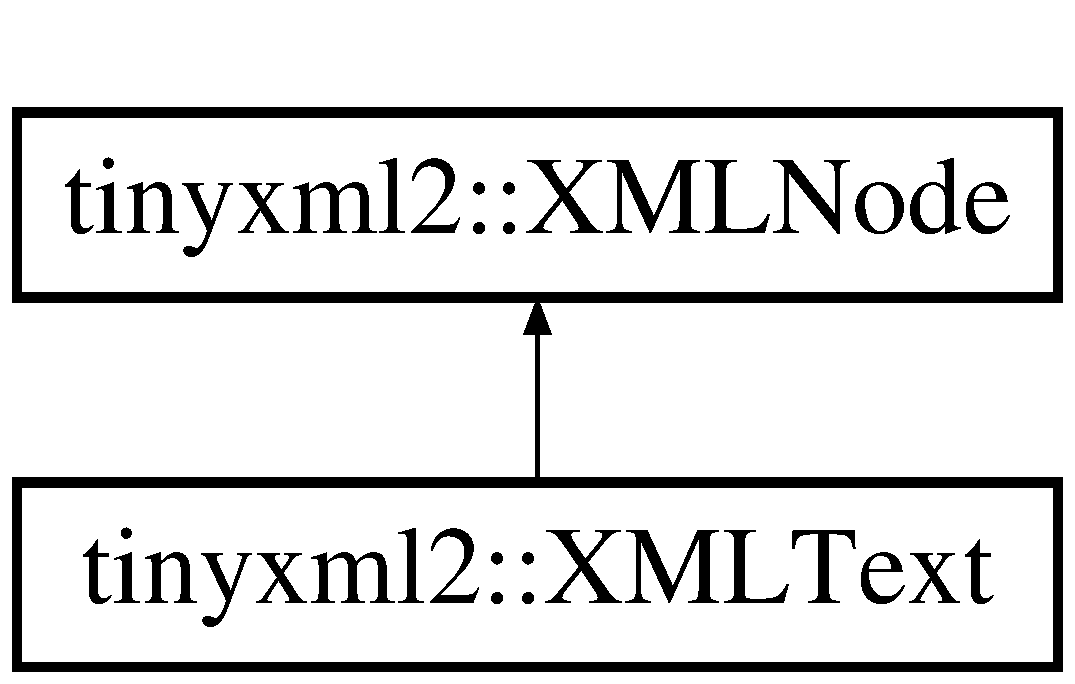
\includegraphics[height=2.000000cm]{classtinyxml2_1_1_x_m_l_text}
\end{center}
\end{figure}
\subsection*{Public Member Functions}
\begin{DoxyCompactItemize}
\item 
virtual bool \hyperlink{classtinyxml2_1_1_x_m_l_text_ae659d4fc7351a7df11c111cbe1ade46f}{Accept} (\hyperlink{classtinyxml2_1_1_x_m_l_visitor}{X\+M\+L\+Visitor} $\ast$visitor) const 
\item 
virtual \hyperlink{classtinyxml2_1_1_x_m_l_text}{X\+M\+L\+Text} $\ast$ \hyperlink{classtinyxml2_1_1_x_m_l_text_ab1213b4ddebe9b17ec7e7040e9f1caf7}{To\+Text} ()\hypertarget{classtinyxml2_1_1_x_m_l_text_ab1213b4ddebe9b17ec7e7040e9f1caf7}{}\label{classtinyxml2_1_1_x_m_l_text_ab1213b4ddebe9b17ec7e7040e9f1caf7}

\begin{DoxyCompactList}\small\item\em Safely cast to Text, or null. \end{DoxyCompactList}\item 
virtual const \hyperlink{classtinyxml2_1_1_x_m_l_text}{X\+M\+L\+Text} $\ast$ {\bfseries To\+Text} () const \hypertarget{classtinyxml2_1_1_x_m_l_text_a1e53cbc60968fe966790a65eaf87baaa}{}\label{classtinyxml2_1_1_x_m_l_text_a1e53cbc60968fe966790a65eaf87baaa}

\item 
void \hyperlink{classtinyxml2_1_1_x_m_l_text_ad080357d76ab7cc59d7651249949329d}{Set\+C\+Data} (bool is\+C\+Data)\hypertarget{classtinyxml2_1_1_x_m_l_text_ad080357d76ab7cc59d7651249949329d}{}\label{classtinyxml2_1_1_x_m_l_text_ad080357d76ab7cc59d7651249949329d}

\begin{DoxyCompactList}\small\item\em Declare whether this should be C\+D\+A\+TA or standard text. \end{DoxyCompactList}\item 
bool \hyperlink{classtinyxml2_1_1_x_m_l_text_a125574fe49da80efbae1349f20d02d41}{C\+Data} () const \hypertarget{classtinyxml2_1_1_x_m_l_text_a125574fe49da80efbae1349f20d02d41}{}\label{classtinyxml2_1_1_x_m_l_text_a125574fe49da80efbae1349f20d02d41}

\begin{DoxyCompactList}\small\item\em Returns true if this is a C\+D\+A\+TA text element. \end{DoxyCompactList}\item 
virtual \hyperlink{classtinyxml2_1_1_x_m_l_node}{X\+M\+L\+Node} $\ast$ \hyperlink{classtinyxml2_1_1_x_m_l_text_af5115f8cc83de2947ed6a9d13e2f88c8}{Shallow\+Clone} (\hyperlink{classtinyxml2_1_1_x_m_l_document}{X\+M\+L\+Document} $\ast$document) const 
\item 
virtual bool \hyperlink{classtinyxml2_1_1_x_m_l_text_a1588aa5d23cb21eb31f36df0aaaa8d66}{Shallow\+Equal} (const \hyperlink{classtinyxml2_1_1_x_m_l_node}{X\+M\+L\+Node} $\ast$compare) const 
\end{DoxyCompactItemize}
\subsection*{Protected Member Functions}
\begin{DoxyCompactItemize}
\item 
{\bfseries X\+M\+L\+Text} (\hyperlink{classtinyxml2_1_1_x_m_l_document}{X\+M\+L\+Document} $\ast$doc)\hypertarget{classtinyxml2_1_1_x_m_l_text_ad9f46d70e61e5386ead93728d8b90267}{}\label{classtinyxml2_1_1_x_m_l_text_ad9f46d70e61e5386ead93728d8b90267}

\item 
char $\ast$ {\bfseries Parse\+Deep} (char $\ast$, \hyperlink{classtinyxml2_1_1_str_pair}{Str\+Pair} $\ast$end\+Tag)\hypertarget{classtinyxml2_1_1_x_m_l_text_ac18d9eec9f12b827b0d02b0847bf279e}{}\label{classtinyxml2_1_1_x_m_l_text_ac18d9eec9f12b827b0d02b0847bf279e}

\end{DoxyCompactItemize}
\subsection*{Friends}
\begin{DoxyCompactItemize}
\item 
class {\bfseries X\+M\+L\+Base}\hypertarget{classtinyxml2_1_1_x_m_l_text_a449202cfc89e7ae5c2f81995476f9ec1}{}\label{classtinyxml2_1_1_x_m_l_text_a449202cfc89e7ae5c2f81995476f9ec1}

\item 
class {\bfseries X\+M\+L\+Document}\hypertarget{classtinyxml2_1_1_x_m_l_text_a4eee3bda60c60a30e4e8cd4ea91c4c6e}{}\label{classtinyxml2_1_1_x_m_l_text_a4eee3bda60c60a30e4e8cd4ea91c4c6e}

\end{DoxyCompactItemize}
\subsection*{Additional Inherited Members}


\subsection{Detailed Description}
X\+ML text.

Note that a text node can have child element nodes, for example\+: \begin{DoxyVerb}<root>This is <b>bold</b></root>
\end{DoxyVerb}


A text node can have 2 ways to output the next. \char`\"{}normal\char`\"{} output and C\+D\+A\+TA. It will default to the mode it was parsed from the X\+ML file and you generally want to leave it alone, but you can change the output mode with \hyperlink{classtinyxml2_1_1_x_m_l_text_ad080357d76ab7cc59d7651249949329d}{Set\+C\+Data()} and query it with \hyperlink{classtinyxml2_1_1_x_m_l_text_a125574fe49da80efbae1349f20d02d41}{C\+Data()}. 

\subsection{Member Function Documentation}
\index{tinyxml2\+::\+X\+M\+L\+Text@{tinyxml2\+::\+X\+M\+L\+Text}!Accept@{Accept}}
\index{Accept@{Accept}!tinyxml2\+::\+X\+M\+L\+Text@{tinyxml2\+::\+X\+M\+L\+Text}}
\subsubsection[{\texorpdfstring{Accept(\+X\+M\+L\+Visitor $\ast$visitor) const }{Accept(XMLVisitor *visitor) const }}]{\setlength{\rightskip}{0pt plus 5cm}bool tinyxml2\+::\+X\+M\+L\+Text\+::\+Accept (
\begin{DoxyParamCaption}
\item[{{\bf X\+M\+L\+Visitor} $\ast$}]{visitor}
\end{DoxyParamCaption}
) const\hspace{0.3cm}{\ttfamily [virtual]}}\hypertarget{classtinyxml2_1_1_x_m_l_text_ae659d4fc7351a7df11c111cbe1ade46f}{}\label{classtinyxml2_1_1_x_m_l_text_ae659d4fc7351a7df11c111cbe1ade46f}
Accept a hierarchical visit of the nodes in the Tiny\+X\+M\+L-\/2 D\+OM. Every node in the X\+ML tree will be conditionally visited and the host will be called back via the \hyperlink{classtinyxml2_1_1_x_m_l_visitor}{X\+M\+L\+Visitor} interface.

This is essentially a S\+AX interface for Tiny\+X\+M\+L-\/2. (Note however it doesn\textquotesingle{}t re-\/parse the X\+ML for the callbacks, so the performance of Tiny\+X\+M\+L-\/2 is unchanged by using this interface versus any other.)

The interface has been based on ideas from\+:


\begin{DoxyItemize}
\item \href{http://www.saxproject.org/}{\tt http\+://www.\+saxproject.\+org/}
\item \href{http://c2.com/cgi/wiki?HierarchicalVisitorPattern}{\tt http\+://c2.\+com/cgi/wiki?\+Hierarchical\+Visitor\+Pattern}
\end{DoxyItemize}

Which are both good references for \char`\"{}visiting\char`\"{}.

An example of using \hyperlink{classtinyxml2_1_1_x_m_l_text_ae659d4fc7351a7df11c111cbe1ade46f}{Accept()}\+: \begin{DoxyVerb}XMLPrinter printer;
tinyxmlDoc.Accept( &printer );
const char* xmlcstr = printer.CStr();
\end{DoxyVerb}
 

Implements \hyperlink{classtinyxml2_1_1_x_m_l_node_a366ad0e9b9ae8d1b18c00f903994b7a9}{tinyxml2\+::\+X\+M\+L\+Node}.

\index{tinyxml2\+::\+X\+M\+L\+Text@{tinyxml2\+::\+X\+M\+L\+Text}!Shallow\+Clone@{Shallow\+Clone}}
\index{Shallow\+Clone@{Shallow\+Clone}!tinyxml2\+::\+X\+M\+L\+Text@{tinyxml2\+::\+X\+M\+L\+Text}}
\subsubsection[{\texorpdfstring{Shallow\+Clone(\+X\+M\+L\+Document $\ast$document) const }{ShallowClone(XMLDocument *document) const }}]{\setlength{\rightskip}{0pt plus 5cm}{\bf X\+M\+L\+Node} $\ast$ tinyxml2\+::\+X\+M\+L\+Text\+::\+Shallow\+Clone (
\begin{DoxyParamCaption}
\item[{{\bf X\+M\+L\+Document} $\ast$}]{document}
\end{DoxyParamCaption}
) const\hspace{0.3cm}{\ttfamily [virtual]}}\hypertarget{classtinyxml2_1_1_x_m_l_text_af5115f8cc83de2947ed6a9d13e2f88c8}{}\label{classtinyxml2_1_1_x_m_l_text_af5115f8cc83de2947ed6a9d13e2f88c8}
Make a copy of this node, but not its children. You may pass in a Document pointer that will be the owner of the new Node. If the \textquotesingle{}document\textquotesingle{} is null, then the node returned will be allocated from the current Document. (this-\/$>$\hyperlink{classtinyxml2_1_1_x_m_l_node_af343d1ef0b45c0020e62d784d7e67a68}{Get\+Document()})

Note\+: if called on a \hyperlink{classtinyxml2_1_1_x_m_l_document}{X\+M\+L\+Document}, this will return null. 

Implements \hyperlink{classtinyxml2_1_1_x_m_l_node_a83e3524e2ecea25eeab630c7ab113627}{tinyxml2\+::\+X\+M\+L\+Node}.

\index{tinyxml2\+::\+X\+M\+L\+Text@{tinyxml2\+::\+X\+M\+L\+Text}!Shallow\+Equal@{Shallow\+Equal}}
\index{Shallow\+Equal@{Shallow\+Equal}!tinyxml2\+::\+X\+M\+L\+Text@{tinyxml2\+::\+X\+M\+L\+Text}}
\subsubsection[{\texorpdfstring{Shallow\+Equal(const X\+M\+L\+Node $\ast$compare) const }{ShallowEqual(const XMLNode *compare) const }}]{\setlength{\rightskip}{0pt plus 5cm}bool tinyxml2\+::\+X\+M\+L\+Text\+::\+Shallow\+Equal (
\begin{DoxyParamCaption}
\item[{const {\bf X\+M\+L\+Node} $\ast$}]{compare}
\end{DoxyParamCaption}
) const\hspace{0.3cm}{\ttfamily [virtual]}}\hypertarget{classtinyxml2_1_1_x_m_l_text_a1588aa5d23cb21eb31f36df0aaaa8d66}{}\label{classtinyxml2_1_1_x_m_l_text_a1588aa5d23cb21eb31f36df0aaaa8d66}
Test if 2 nodes are the same, but don\textquotesingle{}t test children. The 2 nodes do not need to be in the same Document.

Note\+: if called on a \hyperlink{classtinyxml2_1_1_x_m_l_document}{X\+M\+L\+Document}, this will return false. 

Implements \hyperlink{classtinyxml2_1_1_x_m_l_node_ac50408e91e095237f45716092ac2bddc}{tinyxml2\+::\+X\+M\+L\+Node}.



The documentation for this class was generated from the following files\+:\begin{DoxyCompactItemize}
\item 
src/tinyxml2.\+h\item 
src/tinyxml2.\+cpp\end{DoxyCompactItemize}

\hypertarget{classtinyxml2_1_1_x_m_l_unknown}{}\section{tinyxml2\+:\+:X\+M\+L\+Unknown Class Reference}
\label{classtinyxml2_1_1_x_m_l_unknown}\index{tinyxml2\+::\+X\+M\+L\+Unknown@{tinyxml2\+::\+X\+M\+L\+Unknown}}


{\ttfamily \#include $<$tinyxml2.\+h$>$}

Inheritance diagram for tinyxml2\+:\+:X\+M\+L\+Unknown\+:\begin{figure}[H]
\begin{center}
\leavevmode
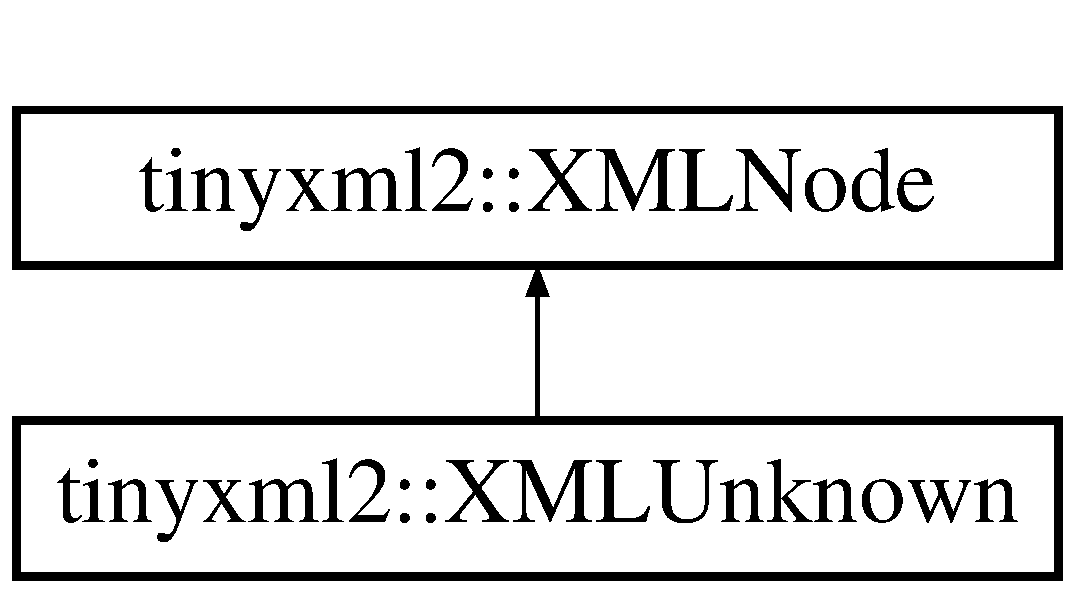
\includegraphics[height=2.000000cm]{classtinyxml2_1_1_x_m_l_unknown}
\end{center}
\end{figure}
\subsection*{Public Member Functions}
\begin{DoxyCompactItemize}
\item 
virtual \hyperlink{classtinyxml2_1_1_x_m_l_unknown}{X\+M\+L\+Unknown} $\ast$ \hyperlink{classtinyxml2_1_1_x_m_l_unknown_af4374856421921cad578c8affae872b6}{To\+Unknown} ()\hypertarget{classtinyxml2_1_1_x_m_l_unknown_af4374856421921cad578c8affae872b6}{}\label{classtinyxml2_1_1_x_m_l_unknown_af4374856421921cad578c8affae872b6}

\begin{DoxyCompactList}\small\item\em Safely cast to an Unknown, or null. \end{DoxyCompactList}\item 
virtual const \hyperlink{classtinyxml2_1_1_x_m_l_unknown}{X\+M\+L\+Unknown} $\ast$ {\bfseries To\+Unknown} () const \hypertarget{classtinyxml2_1_1_x_m_l_unknown_a257987e79955399e6e9f119b58d4bb30}{}\label{classtinyxml2_1_1_x_m_l_unknown_a257987e79955399e6e9f119b58d4bb30}

\item 
virtual bool \hyperlink{classtinyxml2_1_1_x_m_l_unknown_a0d341ab804a1438a474810bb5bd29dd5}{Accept} (\hyperlink{classtinyxml2_1_1_x_m_l_visitor}{X\+M\+L\+Visitor} $\ast$visitor) const 
\item 
virtual \hyperlink{classtinyxml2_1_1_x_m_l_node}{X\+M\+L\+Node} $\ast$ \hyperlink{classtinyxml2_1_1_x_m_l_unknown_aa09fc7cb0cd64d6bb9c5ae00ffc549ec}{Shallow\+Clone} (\hyperlink{classtinyxml2_1_1_x_m_l_document}{X\+M\+L\+Document} $\ast$document) const 
\item 
virtual bool \hyperlink{classtinyxml2_1_1_x_m_l_unknown_a0169df157bf69a092b404ca49621ff1a}{Shallow\+Equal} (const \hyperlink{classtinyxml2_1_1_x_m_l_node}{X\+M\+L\+Node} $\ast$compare) const 
\end{DoxyCompactItemize}
\subsection*{Protected Member Functions}
\begin{DoxyCompactItemize}
\item 
{\bfseries X\+M\+L\+Unknown} (\hyperlink{classtinyxml2_1_1_x_m_l_document}{X\+M\+L\+Document} $\ast$doc)\hypertarget{classtinyxml2_1_1_x_m_l_unknown_a9391eb679598d50baba424e6f1aa367b}{}\label{classtinyxml2_1_1_x_m_l_unknown_a9391eb679598d50baba424e6f1aa367b}

\item 
char $\ast$ {\bfseries Parse\+Deep} (char $\ast$, \hyperlink{classtinyxml2_1_1_str_pair}{Str\+Pair} $\ast$end\+Tag)\hypertarget{classtinyxml2_1_1_x_m_l_unknown_a0e4f3509dee42a4d45a7f0002be568cc}{}\label{classtinyxml2_1_1_x_m_l_unknown_a0e4f3509dee42a4d45a7f0002be568cc}

\end{DoxyCompactItemize}
\subsection*{Friends}
\begin{DoxyCompactItemize}
\item 
class {\bfseries X\+M\+L\+Document}\hypertarget{classtinyxml2_1_1_x_m_l_unknown_a4eee3bda60c60a30e4e8cd4ea91c4c6e}{}\label{classtinyxml2_1_1_x_m_l_unknown_a4eee3bda60c60a30e4e8cd4ea91c4c6e}

\end{DoxyCompactItemize}
\subsection*{Additional Inherited Members}


\subsection{Detailed Description}
Any tag that Tiny\+X\+M\+L-\/2 doesn\textquotesingle{}t recognize is saved as an unknown. It is a tag of text, but should not be modified. It will be written back to the X\+ML, unchanged, when the file is saved.

D\+TD tags get thrown into X\+M\+L\+Unknowns. 

\subsection{Member Function Documentation}
\index{tinyxml2\+::\+X\+M\+L\+Unknown@{tinyxml2\+::\+X\+M\+L\+Unknown}!Accept@{Accept}}
\index{Accept@{Accept}!tinyxml2\+::\+X\+M\+L\+Unknown@{tinyxml2\+::\+X\+M\+L\+Unknown}}
\subsubsection[{\texorpdfstring{Accept(\+X\+M\+L\+Visitor $\ast$visitor) const }{Accept(XMLVisitor *visitor) const }}]{\setlength{\rightskip}{0pt plus 5cm}bool tinyxml2\+::\+X\+M\+L\+Unknown\+::\+Accept (
\begin{DoxyParamCaption}
\item[{{\bf X\+M\+L\+Visitor} $\ast$}]{visitor}
\end{DoxyParamCaption}
) const\hspace{0.3cm}{\ttfamily [virtual]}}\hypertarget{classtinyxml2_1_1_x_m_l_unknown_a0d341ab804a1438a474810bb5bd29dd5}{}\label{classtinyxml2_1_1_x_m_l_unknown_a0d341ab804a1438a474810bb5bd29dd5}
Accept a hierarchical visit of the nodes in the Tiny\+X\+M\+L-\/2 D\+OM. Every node in the X\+ML tree will be conditionally visited and the host will be called back via the \hyperlink{classtinyxml2_1_1_x_m_l_visitor}{X\+M\+L\+Visitor} interface.

This is essentially a S\+AX interface for Tiny\+X\+M\+L-\/2. (Note however it doesn\textquotesingle{}t re-\/parse the X\+ML for the callbacks, so the performance of Tiny\+X\+M\+L-\/2 is unchanged by using this interface versus any other.)

The interface has been based on ideas from\+:


\begin{DoxyItemize}
\item \href{http://www.saxproject.org/}{\tt http\+://www.\+saxproject.\+org/}
\item \href{http://c2.com/cgi/wiki?HierarchicalVisitorPattern}{\tt http\+://c2.\+com/cgi/wiki?\+Hierarchical\+Visitor\+Pattern}
\end{DoxyItemize}

Which are both good references for \char`\"{}visiting\char`\"{}.

An example of using \hyperlink{classtinyxml2_1_1_x_m_l_unknown_a0d341ab804a1438a474810bb5bd29dd5}{Accept()}\+: \begin{DoxyVerb}XMLPrinter printer;
tinyxmlDoc.Accept( &printer );
const char* xmlcstr = printer.CStr();
\end{DoxyVerb}
 

Implements \hyperlink{classtinyxml2_1_1_x_m_l_node_a366ad0e9b9ae8d1b18c00f903994b7a9}{tinyxml2\+::\+X\+M\+L\+Node}.

\index{tinyxml2\+::\+X\+M\+L\+Unknown@{tinyxml2\+::\+X\+M\+L\+Unknown}!Shallow\+Clone@{Shallow\+Clone}}
\index{Shallow\+Clone@{Shallow\+Clone}!tinyxml2\+::\+X\+M\+L\+Unknown@{tinyxml2\+::\+X\+M\+L\+Unknown}}
\subsubsection[{\texorpdfstring{Shallow\+Clone(\+X\+M\+L\+Document $\ast$document) const }{ShallowClone(XMLDocument *document) const }}]{\setlength{\rightskip}{0pt plus 5cm}{\bf X\+M\+L\+Node} $\ast$ tinyxml2\+::\+X\+M\+L\+Unknown\+::\+Shallow\+Clone (
\begin{DoxyParamCaption}
\item[{{\bf X\+M\+L\+Document} $\ast$}]{document}
\end{DoxyParamCaption}
) const\hspace{0.3cm}{\ttfamily [virtual]}}\hypertarget{classtinyxml2_1_1_x_m_l_unknown_aa09fc7cb0cd64d6bb9c5ae00ffc549ec}{}\label{classtinyxml2_1_1_x_m_l_unknown_aa09fc7cb0cd64d6bb9c5ae00ffc549ec}
Make a copy of this node, but not its children. You may pass in a Document pointer that will be the owner of the new Node. If the \textquotesingle{}document\textquotesingle{} is null, then the node returned will be allocated from the current Document. (this-\/$>$\hyperlink{classtinyxml2_1_1_x_m_l_node_af343d1ef0b45c0020e62d784d7e67a68}{Get\+Document()})

Note\+: if called on a \hyperlink{classtinyxml2_1_1_x_m_l_document}{X\+M\+L\+Document}, this will return null. 

Implements \hyperlink{classtinyxml2_1_1_x_m_l_node_a83e3524e2ecea25eeab630c7ab113627}{tinyxml2\+::\+X\+M\+L\+Node}.

\index{tinyxml2\+::\+X\+M\+L\+Unknown@{tinyxml2\+::\+X\+M\+L\+Unknown}!Shallow\+Equal@{Shallow\+Equal}}
\index{Shallow\+Equal@{Shallow\+Equal}!tinyxml2\+::\+X\+M\+L\+Unknown@{tinyxml2\+::\+X\+M\+L\+Unknown}}
\subsubsection[{\texorpdfstring{Shallow\+Equal(const X\+M\+L\+Node $\ast$compare) const }{ShallowEqual(const XMLNode *compare) const }}]{\setlength{\rightskip}{0pt plus 5cm}bool tinyxml2\+::\+X\+M\+L\+Unknown\+::\+Shallow\+Equal (
\begin{DoxyParamCaption}
\item[{const {\bf X\+M\+L\+Node} $\ast$}]{compare}
\end{DoxyParamCaption}
) const\hspace{0.3cm}{\ttfamily [virtual]}}\hypertarget{classtinyxml2_1_1_x_m_l_unknown_a0169df157bf69a092b404ca49621ff1a}{}\label{classtinyxml2_1_1_x_m_l_unknown_a0169df157bf69a092b404ca49621ff1a}
Test if 2 nodes are the same, but don\textquotesingle{}t test children. The 2 nodes do not need to be in the same Document.

Note\+: if called on a \hyperlink{classtinyxml2_1_1_x_m_l_document}{X\+M\+L\+Document}, this will return false. 

Implements \hyperlink{classtinyxml2_1_1_x_m_l_node_ac50408e91e095237f45716092ac2bddc}{tinyxml2\+::\+X\+M\+L\+Node}.



The documentation for this class was generated from the following files\+:\begin{DoxyCompactItemize}
\item 
src/tinyxml2.\+h\item 
src/tinyxml2.\+cpp\end{DoxyCompactItemize}

\hypertarget{classtinyxml2_1_1_x_m_l_util}{}\section{tinyxml2\+:\+:X\+M\+L\+Util Class Reference}
\label{classtinyxml2_1_1_x_m_l_util}\index{tinyxml2\+::\+X\+M\+L\+Util@{tinyxml2\+::\+X\+M\+L\+Util}}
\subsection*{Static Public Member Functions}
\begin{DoxyCompactItemize}
\item 
static const char $\ast$ {\bfseries Skip\+White\+Space} (const char $\ast$p)\hypertarget{classtinyxml2_1_1_x_m_l_util_a9333d20f2a34325b5115ca45849c4b2a}{}\label{classtinyxml2_1_1_x_m_l_util_a9333d20f2a34325b5115ca45849c4b2a}

\item 
static char $\ast$ {\bfseries Skip\+White\+Space} (char $\ast$p)\hypertarget{classtinyxml2_1_1_x_m_l_util_aa48025be8843ec5a79b65579d31bd8fc}{}\label{classtinyxml2_1_1_x_m_l_util_aa48025be8843ec5a79b65579d31bd8fc}

\item 
static bool {\bfseries Is\+White\+Space} (char p)\hypertarget{classtinyxml2_1_1_x_m_l_util_a357ec3af8fc433d19023a815f45e8e33}{}\label{classtinyxml2_1_1_x_m_l_util_a357ec3af8fc433d19023a815f45e8e33}

\item 
static bool {\bfseries Is\+Name\+Start\+Char} (unsigned char ch)\hypertarget{classtinyxml2_1_1_x_m_l_util_abe106a69ac4d942a4381a4d9dfd0e0bd}{}\label{classtinyxml2_1_1_x_m_l_util_abe106a69ac4d942a4381a4d9dfd0e0bd}

\item 
static bool {\bfseries Is\+Name\+Char} (unsigned char ch)\hypertarget{classtinyxml2_1_1_x_m_l_util_a04b17341538fa11752f24b4301d19485}{}\label{classtinyxml2_1_1_x_m_l_util_a04b17341538fa11752f24b4301d19485}

\item 
static bool {\bfseries String\+Equal} (const char $\ast$p, const char $\ast$q, int n\+Char=I\+N\+T\+\_\+\+M\+AX)\hypertarget{classtinyxml2_1_1_x_m_l_util_acfcd287cacfd2533e1bc9ea4dfb56602}{}\label{classtinyxml2_1_1_x_m_l_util_acfcd287cacfd2533e1bc9ea4dfb56602}

\item 
static bool {\bfseries Is\+U\+T\+F8\+Continuation} (char p)\hypertarget{classtinyxml2_1_1_x_m_l_util_ad7fd82e0fe610d73ef7bf9f359f104a3}{}\label{classtinyxml2_1_1_x_m_l_util_ad7fd82e0fe610d73ef7bf9f359f104a3}

\item 
static const char $\ast$ {\bfseries Read\+B\+OM} (const char $\ast$p, bool $\ast$has\+B\+OM)\hypertarget{classtinyxml2_1_1_x_m_l_util_ae9bcb2bc3cd6475fdc644c8c17790555}{}\label{classtinyxml2_1_1_x_m_l_util_ae9bcb2bc3cd6475fdc644c8c17790555}

\item 
static const char $\ast$ {\bfseries Get\+Character\+Ref} (const char $\ast$p, char $\ast$value, int $\ast$length)\hypertarget{classtinyxml2_1_1_x_m_l_util_a5a96e5144a8d693dc4bcd783d9964648}{}\label{classtinyxml2_1_1_x_m_l_util_a5a96e5144a8d693dc4bcd783d9964648}

\item 
static void {\bfseries Convert\+U\+T\+F32\+To\+U\+T\+F8} (unsigned long input, char $\ast$output, int $\ast$length)\hypertarget{classtinyxml2_1_1_x_m_l_util_a31c00d5c5dfb38382de1dfcaf4be3595}{}\label{classtinyxml2_1_1_x_m_l_util_a31c00d5c5dfb38382de1dfcaf4be3595}

\item 
static void {\bfseries To\+Str} (int v, char $\ast$buffer, int buffer\+Size)\hypertarget{classtinyxml2_1_1_x_m_l_util_a3cd6c703d49b9d51bdf0f4ff6aa021c7}{}\label{classtinyxml2_1_1_x_m_l_util_a3cd6c703d49b9d51bdf0f4ff6aa021c7}

\item 
static void {\bfseries To\+Str} (unsigned v, char $\ast$buffer, int buffer\+Size)\hypertarget{classtinyxml2_1_1_x_m_l_util_ac00c2e52c1c36dab3ff41d86a9bf60f9}{}\label{classtinyxml2_1_1_x_m_l_util_ac00c2e52c1c36dab3ff41d86a9bf60f9}

\item 
static void {\bfseries To\+Str} (bool v, char $\ast$buffer, int buffer\+Size)\hypertarget{classtinyxml2_1_1_x_m_l_util_adba0718527ae9e80f663a71ea325cb11}{}\label{classtinyxml2_1_1_x_m_l_util_adba0718527ae9e80f663a71ea325cb11}

\item 
static void {\bfseries To\+Str} (float v, char $\ast$buffer, int buffer\+Size)\hypertarget{classtinyxml2_1_1_x_m_l_util_a8957ad44fee5fa02ba52d73aad4d0a31}{}\label{classtinyxml2_1_1_x_m_l_util_a8957ad44fee5fa02ba52d73aad4d0a31}

\item 
static void {\bfseries To\+Str} (double v, char $\ast$buffer, int buffer\+Size)\hypertarget{classtinyxml2_1_1_x_m_l_util_a1cd141e50980fcddd6bf9af5de4b1db7}{}\label{classtinyxml2_1_1_x_m_l_util_a1cd141e50980fcddd6bf9af5de4b1db7}

\item 
static bool {\bfseries To\+Int} (const char $\ast$str, int $\ast$value)\hypertarget{classtinyxml2_1_1_x_m_l_util_ad4df4023d11ee3fca9689c49b9707323}{}\label{classtinyxml2_1_1_x_m_l_util_ad4df4023d11ee3fca9689c49b9707323}

\item 
static bool {\bfseries To\+Unsigned} (const char $\ast$str, unsigned $\ast$value)\hypertarget{classtinyxml2_1_1_x_m_l_util_a210c8637d5eb4ce3d4625294af0efc2f}{}\label{classtinyxml2_1_1_x_m_l_util_a210c8637d5eb4ce3d4625294af0efc2f}

\item 
static bool {\bfseries To\+Bool} (const char $\ast$str, bool $\ast$value)\hypertarget{classtinyxml2_1_1_x_m_l_util_ae5b03e0a1ca5d42052a7ac540f7aa12a}{}\label{classtinyxml2_1_1_x_m_l_util_ae5b03e0a1ca5d42052a7ac540f7aa12a}

\item 
static bool {\bfseries To\+Float} (const char $\ast$str, float $\ast$value)\hypertarget{classtinyxml2_1_1_x_m_l_util_a399e71edb5f29d61ea81d91ee0332bb9}{}\label{classtinyxml2_1_1_x_m_l_util_a399e71edb5f29d61ea81d91ee0332bb9}

\item 
static bool {\bfseries To\+Double} (const char $\ast$str, double $\ast$value)\hypertarget{classtinyxml2_1_1_x_m_l_util_ad8f75ac140fb19c1c6e164a957c4cd53}{}\label{classtinyxml2_1_1_x_m_l_util_ad8f75ac140fb19c1c6e164a957c4cd53}

\end{DoxyCompactItemize}


The documentation for this class was generated from the following files\+:\begin{DoxyCompactItemize}
\item 
src/tinyxml2.\+h\item 
src/tinyxml2.\+cpp\end{DoxyCompactItemize}

\hypertarget{classtinyxml2_1_1_x_m_l_visitor}{}\section{tinyxml2\+:\+:X\+M\+L\+Visitor Class Reference}
\label{classtinyxml2_1_1_x_m_l_visitor}\index{tinyxml2\+::\+X\+M\+L\+Visitor@{tinyxml2\+::\+X\+M\+L\+Visitor}}


{\ttfamily \#include $<$tinyxml2.\+h$>$}

Inheritance diagram for tinyxml2\+:\+:X\+M\+L\+Visitor\+:\begin{figure}[H]
\begin{center}
\leavevmode
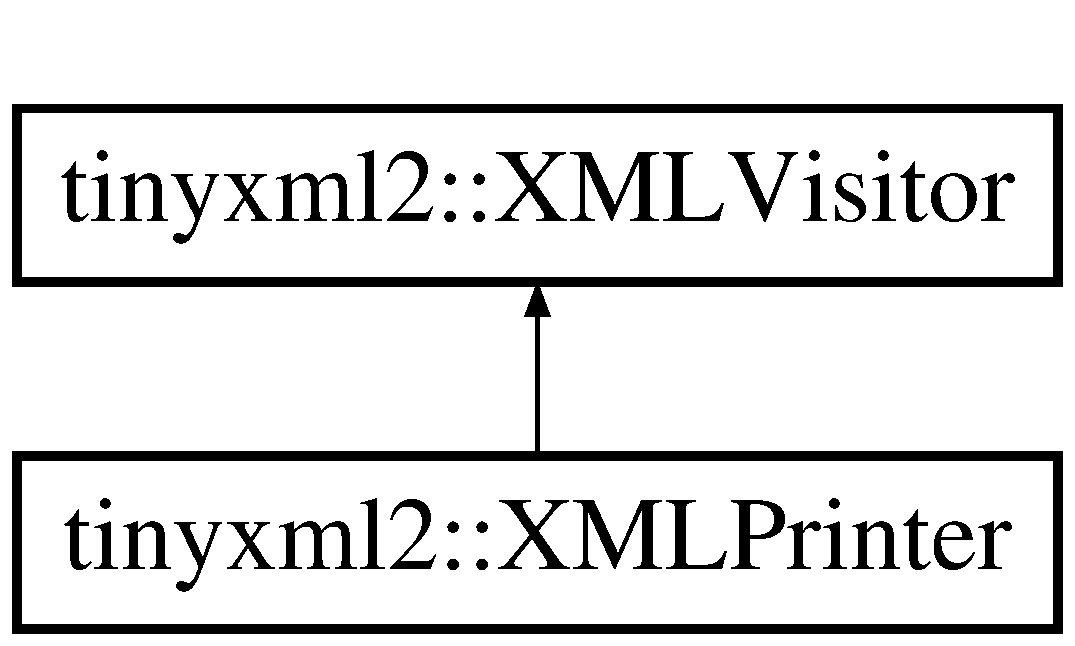
\includegraphics[height=2.000000cm]{classtinyxml2_1_1_x_m_l_visitor}
\end{center}
\end{figure}
\subsection*{Public Member Functions}
\begin{DoxyCompactItemize}
\item 
virtual bool \hyperlink{classtinyxml2_1_1_x_m_l_visitor_acb3c22fc5f60eb9db98f533f2761f67d}{Visit\+Enter} (const \hyperlink{classtinyxml2_1_1_x_m_l_document}{X\+M\+L\+Document} \&)\hypertarget{classtinyxml2_1_1_x_m_l_visitor_acb3c22fc5f60eb9db98f533f2761f67d}{}\label{classtinyxml2_1_1_x_m_l_visitor_acb3c22fc5f60eb9db98f533f2761f67d}

\begin{DoxyCompactList}\small\item\em Visit a document. \end{DoxyCompactList}\item 
virtual bool \hyperlink{classtinyxml2_1_1_x_m_l_visitor_a170e9989cd046ba904f302d087e07086}{Visit\+Exit} (const \hyperlink{classtinyxml2_1_1_x_m_l_document}{X\+M\+L\+Document} \&)\hypertarget{classtinyxml2_1_1_x_m_l_visitor_a170e9989cd046ba904f302d087e07086}{}\label{classtinyxml2_1_1_x_m_l_visitor_a170e9989cd046ba904f302d087e07086}

\begin{DoxyCompactList}\small\item\em Visit a document. \end{DoxyCompactList}\item 
virtual bool \hyperlink{classtinyxml2_1_1_x_m_l_visitor_af97980a17dd4e37448b181f5ddfa92b5}{Visit\+Enter} (const \hyperlink{classtinyxml2_1_1_x_m_l_element}{X\+M\+L\+Element} \&, const \hyperlink{classtinyxml2_1_1_x_m_l_attribute}{X\+M\+L\+Attribute} $\ast$)\hypertarget{classtinyxml2_1_1_x_m_l_visitor_af97980a17dd4e37448b181f5ddfa92b5}{}\label{classtinyxml2_1_1_x_m_l_visitor_af97980a17dd4e37448b181f5ddfa92b5}

\begin{DoxyCompactList}\small\item\em Visit an element. \end{DoxyCompactList}\item 
virtual bool \hyperlink{classtinyxml2_1_1_x_m_l_visitor_a772f10ddc83f881956d32628faa16eb6}{Visit\+Exit} (const \hyperlink{classtinyxml2_1_1_x_m_l_element}{X\+M\+L\+Element} \&)\hypertarget{classtinyxml2_1_1_x_m_l_visitor_a772f10ddc83f881956d32628faa16eb6}{}\label{classtinyxml2_1_1_x_m_l_visitor_a772f10ddc83f881956d32628faa16eb6}

\begin{DoxyCompactList}\small\item\em Visit an element. \end{DoxyCompactList}\item 
virtual bool \hyperlink{classtinyxml2_1_1_x_m_l_visitor_adc75bd459fc7ba8223b50f0616767f9a}{Visit} (const \hyperlink{classtinyxml2_1_1_x_m_l_declaration}{X\+M\+L\+Declaration} \&)\hypertarget{classtinyxml2_1_1_x_m_l_visitor_adc75bd459fc7ba8223b50f0616767f9a}{}\label{classtinyxml2_1_1_x_m_l_visitor_adc75bd459fc7ba8223b50f0616767f9a}

\begin{DoxyCompactList}\small\item\em Visit a declaration. \end{DoxyCompactList}\item 
virtual bool \hyperlink{classtinyxml2_1_1_x_m_l_visitor_af30233565856480ea48b6fa0d6dec65b}{Visit} (const \hyperlink{classtinyxml2_1_1_x_m_l_text}{X\+M\+L\+Text} \&)\hypertarget{classtinyxml2_1_1_x_m_l_visitor_af30233565856480ea48b6fa0d6dec65b}{}\label{classtinyxml2_1_1_x_m_l_visitor_af30233565856480ea48b6fa0d6dec65b}

\begin{DoxyCompactList}\small\item\em Visit a text node. \end{DoxyCompactList}\item 
virtual bool \hyperlink{classtinyxml2_1_1_x_m_l_visitor_acc8147fb5a85f6c65721654e427752d7}{Visit} (const \hyperlink{classtinyxml2_1_1_x_m_l_comment}{X\+M\+L\+Comment} \&)\hypertarget{classtinyxml2_1_1_x_m_l_visitor_acc8147fb5a85f6c65721654e427752d7}{}\label{classtinyxml2_1_1_x_m_l_visitor_acc8147fb5a85f6c65721654e427752d7}

\begin{DoxyCompactList}\small\item\em Visit a comment node. \end{DoxyCompactList}\item 
virtual bool \hyperlink{classtinyxml2_1_1_x_m_l_visitor_a14e4748387c34bf53d24e8119bb1f292}{Visit} (const \hyperlink{classtinyxml2_1_1_x_m_l_unknown}{X\+M\+L\+Unknown} \&)\hypertarget{classtinyxml2_1_1_x_m_l_visitor_a14e4748387c34bf53d24e8119bb1f292}{}\label{classtinyxml2_1_1_x_m_l_visitor_a14e4748387c34bf53d24e8119bb1f292}

\begin{DoxyCompactList}\small\item\em Visit an unknown node. \end{DoxyCompactList}\end{DoxyCompactItemize}


\subsection{Detailed Description}
Implements the interface to the \char`\"{}\+Visitor pattern\char`\"{} (see the Accept() method.) If you call the Accept() method, it requires being passed a \hyperlink{classtinyxml2_1_1_x_m_l_visitor}{X\+M\+L\+Visitor} class to handle callbacks. For nodes that contain other nodes (Document, Element) you will get called with a Visit\+Enter/\+Visit\+Exit pair. Nodes that are always leafs are simply called with \hyperlink{classtinyxml2_1_1_x_m_l_visitor_adc75bd459fc7ba8223b50f0616767f9a}{Visit()}.

If you return \textquotesingle{}true\textquotesingle{} from a Visit method, recursive parsing will continue. If you return false, {\bfseries no children of this node or its siblings} will be visited.

All flavors of Visit methods have a default implementation that returns \textquotesingle{}true\textquotesingle{} (continue visiting). You need to only override methods that are interesting to you.

Generally Accept() is called on the \hyperlink{classtinyxml2_1_1_x_m_l_document}{X\+M\+L\+Document}, although all nodes support visiting.

You should never change the document from a callback.

\begin{DoxySeeAlso}{See also}
\hyperlink{classtinyxml2_1_1_x_m_l_node_a366ad0e9b9ae8d1b18c00f903994b7a9}{X\+M\+L\+Node\+::\+Accept()} 
\end{DoxySeeAlso}


The documentation for this class was generated from the following file\+:\begin{DoxyCompactItemize}
\item 
src/tinyxml2.\+h\end{DoxyCompactItemize}

%--- End generated contents ---

% Index
\backmatter
\newpage
\phantomsection
\clearemptydoublepage
\addcontentsline{toc}{chapter}{Index}
\printindex

\end{document}
